\documentclass[a4paper,12pt]{report}
\usepackage{a4wide}

%\documentclass[a5paper,10pt]{book}
%\usepackage[top=23mm, bottom=18mm, left=15mm, right=25mm]{geometry}
%\geometry{papersize={170mm,220mm}}


\usepackage[utf8x]{inputenc}
\usepackage[danish]{babel}

\usepackage{xr-hyper} %Externe hyper-ref
\usepackage[colorlinks=true, hyperindex=true, linkcolor=minmblaa, citecolor=minmblaa, urlcolor=minmblaa]{hyperref}
\hypersetup{colorlinks=true,filecolor=minmblaa,bookmarksnumbered=true} %Til hyperreferencer. Referencer med farver
\usepackage{needspace} % giver mulighed for at kræve at der skal være et antal tomme linier på siden før ellers indsættes et sideskift.
\usepackage{framed} %Bokse
\usepackage{wrapfig}

\usepackage{amsmath,amsfonts,amssymb,amsthm,mathtools} %Matematikpakker

\setlength{\parindent}{0mm} %Ingen Indhak i første linje i afsnit

\usepackage{color} %Farvepakke

\usepackage{array}
\usepackage{colortbl}
\usepackage{multirow} %Til at flette rækker i tabeller.

\usepackage{verbatim,mhchem}



	% DOWNLOAD FRA: http://sarovar.org/frs/?group_id=52&release_id=97
	% Læg i directory for hoved TEX fil
%\usepackage[draft]{pdfdraftcopy}
%\draftstring{Licens: Kasper Langt Mellemnavn Skårhøj}
%\draftfontsize{30}
	%\draftfontfamily{hlh}
	%\draftangle{45}
	%\definecolor{mycolor}{rgb}{.825,.855,1}
	%\draftcolor{mycolor}
	%\draftfontattrib



% = Sidehoved =
\usepackage{fancyhdr}
\pagestyle{fancy}
\renewcommand{\sectionmark}[1]{\markright{\protect\titlegraphic{dturoed}\textcolor{dtugraa}{\thesection~\MakeUppercase{#1}}}} % \thesection.\
\fancyhead{}
\fancyfoot{}
\fancyhead[R]{\titlefont\thepage}
\fancyhead[C]{}
\fancyhead[L]{\titlefont \small eNote \MakeUppercase{~\thechapter}~\hspace*{1ex}\rightmark}
\renewcommand\headrulewidth{0pt}
\fancypagestyle{plain}{\fancyfoot[C]{}}% {\titlefont\footnotesize\thepage}}
\setlength{\headheight}{15pt}


% = Længder
%\newlength{\envtblsep}\setlength{\envtblsep}{1\FrameSep}
\newlength{\obsl}\setlength{\obsl}{\textwidth-1.2cm-13.2pt}

% Includes:

% =     Fonts (select one)    =
\usepackage{mathpazo}\linespread{1.05} % Palatino needs more leading (space between lines)
\usepackage{bm} % bold math, must be loaded after the fontpackages

% % Til overskrifter
\DeclareTextFontCommand{\th}{\fontencoding{T1}\fontfamily{phv}\fontseries{b}\selectfont}
\newcommand\titlefont{\fontencoding{T1}\fontfamily{phv}\selectfont}


% =     PGF grafik      =
\usepackage{tikz}
\newcommand\titlegraphic[1]{%
\tikz[baseline] %
\draw[thick,color=#1]
(0pt  ,-0.25em) -- (0pt  ,0.85em)
(2.5pt,-0.25em) -- (2.5pt,0.85em)
(5pt  ,-0.25em) -- (5pt  ,0.85em)
(7.5pt,-0.25em) -- (7.5pt,0.85em);\hspace*{0.8ex} %
}

\newcommand\titlegraphicwide[1]{%
\tikz[baseline] %
\draw[line width=0.8mm,color=#1]
(0pt  ,-0.25em) -- (0pt  ,0.85em)
(4.5pt,-0.25em) -- (4.5pt,0.85em)
(9pt  ,-0.25em) -- (9pt  ,0.85em)
(13.5pt,-0.25em) -- (13.5pt,0.85em);\hspace*{0.8ex} %
}


% =      Title Layout      =
\usepackage{titlesec}
\makeatletter
\titleformat{\chapter}
	[display] % Shape
	{\titlefont\Huge\flushleft} % Title and label format
	{\titlefont\LARGE\bfseries \titlegraphicwide{dturoed}\textcolor{dtugraa}{\@chapapp~\thechapter}} % label
	{0.9em} % label/title separation
	{} % before code
	[] % after code
\makeatother
\titleformat{\section}
	[hang] % Shape
	{\titlefont\Large\flushleft} % Title and label format
	{\thesection} % label
	{0.9em} % label/title separation
	{} % before code
	[] % after code
\titleformat{\subsection}
	[hang] % Shape
	{\titlefont\large} % Title and label format
	{\thesubsection} % label
	{0.9em} % label/title separation
	{} % before code
	[] % after code
\titlespacing{\subsection}{0pt}{*6}{*1.5}
\titleformat{\subsubsection}
	[hang] % Shape
	{\titlefont} % Title and label format
	{\thesubsubsection} % label
	{0.9em} % label/title separation
	{} % before code
	[] % after code



% = Farver
\definecolor{dturoed}{rgb}{0.6, 0.0, 0.0}
\definecolor{dtugraa}{rgb}{0.5, 0.5, 0.5}	% Lidt mørkere. Korrekt = 0.4
\definecolor{mingroenstreg}{rgb}{0.4,0.8,0}	% Sekundærfarve 14 : 102/204/0	(Forårsgrøn) -> Eksempler
\definecolor{mingroen}{rgb}{0.32,0.64,0}		% Sekundærfarve 14, 80% mørkere (tekst)
\definecolor{minorangestreg}{rgb}{1,0.6,0}		% Sekundærfarve 1 : 255/153/0	(Orange) -> Opgaver
\definecolor{minorange}{rgb}{0.8,0.48,0}		% Sekundærfarve 1 , 80% mørkere (tekst)

\definecolor{minblaa}{rgb}{0.2,0.4,0.8}	% Sekundærfarve 13 , 51/102/204 	( Blå -> Definitioner etc)
\definecolor{minmblaa}{rgb}{0.16,0.32,0.64}	% Sekundærfarve 13 , 80% mørkere (tekst)
\definecolor{thmbackground}{rgb}{0.97,.97, 0.99}	% Farve 13 - lys baggrund

\definecolor{mingraastreg}{rgb}{.5,.5,.5}
\definecolor{hvadbackground}{rgb}{0.97,.97, 0.97}
\definecolor{sumgul}{rgb}{1,1,.8}

\definecolor{hjmopgfarve}{rgb}{.96,1,.96}


% = Counter
\newcounter{evncount}[chapter]
\setcounter{evncount}{0}
\renewcommand{\theevncount}{\thechapter.\arabic{evncount}}
\renewcommand{\theequation}{\thechapter-\arabic{equation}}


% = Eksempler = example =
\newenvironment{example}[1][]{
	\refstepcounter{evncount}
	\setlength{\obsl}{\textwidth-1.2cm-13.2pt-9pt} % fix width of the info envirnment%
	\def\FrameCommand{ 
		\textcolor{mingroenstreg}{\vrule width 4pt} 
		\hspace{5pt} 
	}%
	\MakeFramed{\advance\hsize-\width \FrameRestore}%
	\needspace{3\baselineskip}
	\titlegraphic{mingroen}
	\textcolor{mingroen}{
		\th{Eksempel \theevncount \hspace*{5mm} #1}
	} 
	\vspace*{3mm}%
	\begin{small}
	\par
}
{
	\end{small}
	\endMakeFramed
}


% = Opgaver = exercise =
\newenvironment{exercise}[1][]{
	\refstepcounter{evncount}
	\setlength{\obsl}{\textwidth-1.2cm-13.2pt-9pt}% fix width of the info envirnment%
	\def\FrameCommand{
		\textcolor{minorangestreg}{\vrule width 4pt}
		\hspace{5pt}
	}%
	\MakeFramed{\advance\hsize-\width \FrameRestore}%
	\needspace{3\baselineskip}
	\titlegraphic{minorange}
	\textcolor{minorange}{
		\th{Opgave \theevncount \hspace*{5mm} #1}
	} 
	\vspace*{3mm}%
	\begin{small}
	\par
}
{
	\end{small}
	\endMakeFramed
}


% = Bevis
\newenvironment{bevis}{
	\setlength{\obsl}{\textwidth-1.2cm-13.2pt-9pt} % fix width of the info envirnment%
	\def\FrameCommand{
		\textcolor{mingraastreg}{\vrule width 4pt} 
		\hspace{5pt}
	}%
	\MakeFramed{\advance\hsize-\width \FrameRestore}%
	\needspace{3\baselineskip}
	\titlegraphic{black}
	\textcolor{black}{
		\th{Bevis}
	}
	\vspace*{3mm}%
	\begin{small}
	\par
}
{
	\bevisslut 
	\end{small}
	\endMakeFramed
}


% = Definition =
\newenvironment{definition}[1][]{
	\vspace{4mm}
	\pagebreak[1]
	\setlength{\obsl}{\textwidth-1.2cm-2\FrameSep-13.2pt}%
	\def\FrameCommand{
		\fboxsep=\FrameSep\fcolorbox{minblaa}{thmbackground}
	}
	\begin{minipage}{\textwidth}
	\MakeFramed{\advance\hsize-\width\FrameRestore}
	\refstepcounter{evncount}
	\titlegraphic{minblaa}
	\textcolor{minmblaa}{
		\th{Definition \theevncount \hspace*{5mm} #1}
	}
	\vspace*{3mm}
	\par
}
{
	\endMakeFramed 
	\end{minipage}
	\vspace{4mm}
}


% = Theorem =
\newenvironment{theorem}[1][]{
	\vspace{4mm}
	\pagebreak[1]%
	\setlength{\obsl}{\textwidth-1.2cm-2\FrameSep-13.2pt}%
	\def\FrameCommand{
		\fboxsep=\FrameSep\fcolorbox{minblaa}{thmbackground}
	}%
	\begin{minipage}{\textwidth}
	\MakeFramed{\advance\hsize-\width\FrameRestore}%
	\refstepcounter{evncount}
	\titlegraphic{minblaa}
	\textcolor{minmblaa}{
		\th{Sætning \theevncount \hspace*{5mm} #1}
	}
	\vspace*{3mm}
	\par
}
{
	\endMakeFramed 
	\end{minipage}
	\vspace{4mm}
}


% = Lemma =
\newenvironment{lemma}[1][]{
	\vspace{4mm}
	\pagebreak[1]
	\setlength{\obsl}{\textwidth-1.2cm-2\FrameSep-13.2pt}%
	\def\FrameCommand{
		\fboxsep=\FrameSep \fcolorbox{minblaa}{thmbackground}
	}
	\begin{minipage}{\textwidth} 
	\MakeFramed{\advance\hsize-\width \FrameRestore}
	\refstepcounter{evncount}
	\titlegraphic{minblaa}
	\textcolor{minmblaa}{
		\th{Hjælpesætning \theevncount \hspace*{5mm} #1}
	}
	\vspace*{3mm}
	\par
}
{
	\endMakeFramed 
	\end{minipage}
	\vspace{4mm}
}


% = Corollary =
\newenvironment{corollary}[1][]{
	\vspace{4mm}
	\pagebreak[1]
	\setlength{\obsl}{\textwidth-1.2cm-2\FrameSep-13.2pt}%
	\def\FrameCommand{
		\fboxsep=\FrameSep \fcolorbox{minblaa}{thmbackground}
	}
	\begin{minipage}{\textwidth} 
	\MakeFramed{\advance\hsize-\width \FrameRestore}
	\refstepcounter{evncount}
	\titlegraphic{minblaa}
	\textcolor{minmblaa}{
		\th{Følgesætning \theevncount \hspace*{5mm} #1}
	}
	\vspace*{3mm}
	\par
}
{
	\endMakeFramed 
	\end{minipage}
	\vspace{4mm}
}


% = Metode = method
\newenvironment{method}[1][]{
	\vspace{4mm}
	\pagebreak[1]
	\setlength{\obsl}{\textwidth-1.2cm-2\FrameSep-13.2pt}%
	\def\FrameCommand{
		\fboxsep=\FrameSep \fcolorbox{black}{hvadbackground}
	}
	\begin{minipage}{\textwidth} 
	\MakeFramed{\advance\hsize-\width \FrameRestore}
	\refstepcounter{evncount}
	\titlegraphic{black}
	\textcolor{black}{
		\th{Metode \theevncount \hspace*{5mm} #1}
	}
	\vspace*{3mm}
	\par
}
{
	\endMakeFramed
	\end{minipage}
	\vspace{4mm}
}


% = Forklaring = explain =
\newenvironment{explain}[1][]{
	\vspace{4mm}
	\pagebreak[1]
	\setlength{\obsl}{\textwidth-1.2cm-2\FrameSep-13.2pt}%
	\def\FrameCommand{
		\fboxsep=\FrameSep \fcolorbox{black}{hvadbackground}
	}
	\MakeFramed{\advance\hsize-\width \FrameRestore}
	\refstepcounter{evncount}
	\titlegraphic{black}
	\textcolor{black}{
		\th{Forklaring \theevncount \hspace*{5mm} #1}
	}
	\vspace*{3mm}
	\par
}
{
	\endMakeFramed
	\vspace{4mm}
}


% = Bemærkning = remark =
\newenvironment{remark}[1][]{
	\vspace{4mm}
	\pagebreak[1]
	\setlength{\obsl}{\textwidth-1.2cm-2\FrameSep-13.2pt}%
	\def\FrameCommand{
		\fboxsep=\FrameSep \fcolorbox{black}{hvadbackground}
	}
	\begin{minipage}{\textwidth} 
	\MakeFramed{\advance\hsize-\width \FrameRestore}
	\refstepcounter{evncount}
	\titlegraphic{black}
	\textcolor{black}{
		\th{Bemærkning \theevncount \hspace*{5mm} #1}
	}
	\vspace*{3mm}
	\par
}
{
	\endMakeFramed 
	\end{minipage}
	\vspace{4mm}
}







% = OBS! = obs =
\newenvironment{obs}{\vspace{4mm}\par%
\begin{tabular}{m{1.2cm}<{\hspace*{2mm}}@{}|m{\obsl}@{}}\hspace*{-4pt}\raggedleft
\includegraphics[width=1.1cm]{../Strukturfiler/FIGS/Alert01} & \begin{minipage}{\obsl}}{\end{minipage}\\ \end{tabular}\vspace{4mm}\par}


% = INFO = info =
\newenvironment{info}{\vspace{4mm}\par%
\begin{tabular}{m{1.2cm}<{\hspace*{2mm}}@{}|m{\obsl}@{}}\hspace*{-4pt}\raggedleft
\includegraphics[width=1.1cm]{../Strukturfiler/FIGS/Info01} & \begin{minipage}{\obsl}}{\end{minipage}\\ \end{tabular}\vspace{4mm}\par}


% = THINK= think =
\newenvironment{think}{\vspace{4mm}\par%
\begin{tabular}{m{1.2cm}<{\hspace*{2mm}}@{}|m{\obsl}@{}}\hspace*{-4pt}\raggedleft
\includegraphics[width=0.7cm]{../Strukturfiler/FIGS/ChessPiece} & \begin{minipage}{\obsl}}{\end{minipage}\\ \end{tabular}\vspace{4mm}\par}


% = AHA= aha =
\newenvironment{aha}{\vspace{4mm}\par%
\begin{tabular}{m{1.2cm}<{\hspace*{2mm}}@{}|m{\obsl}@{}}\hspace*{-4pt}\raggedleft
\includegraphics[width=1.1cm]{../Strukturfiler/FIGS/Think} & \begin{minipage}{\obsl}}{\end{minipage}\\ \end{tabular}\vspace{4mm}\par}


% = BUILDUP= build =
\newenvironment{build}{\vspace{4mm}\par%
\begin{tabular}{m{1.2cm}<{\hspace*{2mm}}@{}|m{\obsl}@{}}\hspace*{-4pt}\raggedleft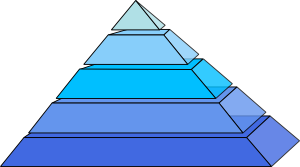
\includegraphics[width=1.1cm]{../Strukturfiler/FIGS/BluePyramid} & \begin{minipage}{\obsl}}{\end{minipage}\\ \end{tabular}\vspace{4mm}\newline}


% = Forudsætning = basis
\newenvironment{basis}{\begin{flushleft} \begin{itshape} }{\end{itshape} \end{flushleft}}


% = Opsummering =
\newenvironment{summary}{\clearpage\pagecolor{sumgul}\section{Opsummering}}{\newpage\pagecolor{white}}











% = Counter
\newcounter{opgavecount}[section]
\setcounter{opgavecount}{0}
\newcounter{spgcount}[opgavecount]
\setcounter{spgcount}{0}
\renewcommand{\thespgcount}{\alph{spgcount})}



% = EXERCISE = (DIVIDER)

\newcommand{\exercisebegin}[1][]{\bigskip\needspace{3\baselineskip}\refstepcounter{opgavecount}\titlegraphic{mingroen}\textcolor{mingroen}{\th{Opgave \theopgavecount \hspace*{1cm} #1}}\medskip\par}

% = QUIZEXERCISE = (DIVIDER)

\newcommand{\quizexercisebegin}[1][]{\bigskip\needspace{3\baselineskip}\refstepcounter{opgavecount}\titlegraphic{mingroen}\textcolor{mingroen}{\th{Quiz-Opgave \theopgavecount \hspace*{1cm} #1}}\medskip\par}

% = QUESTION =

\newenvironment{question}{\refstepcounter{spgcount}\begin{itemize}\item[\thespgcount]}{\end{itemize}\hspace*{\fill}}

% = VINK =

\newenvironment{vink}{\begin{tabular}{m{.9cm}<{\hspace*{2mm}}@{}|m{\obsl}@{}}\hspace*{-4pt}\raggedleft
\includegraphics[width=.9cm]{../Strukturfiler/FIGS/Think} & \begin{minipage}{\obsl}}{\end{minipage}\\ \end{tabular}\medskip\\}
	
% = FACIT =

\newenvironment{facit}{\begin{tabular}{m{.9cm}<{\hspace*{2mm}}@{}|m{\obsl}@{}}\hspace*{-4pt}\raggedleft
\includegraphics[width=.9cm]{../Strukturfiler/FIGS/Check} & \begin{minipage}{\obsl}}{\end{minipage}\\ \end{tabular}\medskip\\}








\newcommand{\afsnit}[1]{\bigskip\th{\titlegraphic{mingroen}\textcolor{mingroen}{#1}} \\ \rule[7pt]{.4\textwidth}{1pt} \vspace*{-2.5mm}\par}

% (DIVIDER):
\newcommand{\ugedagdatotitel}[4]{\pagebreak[4]\section{Semesteruge #1 -- #2 Dag \hspace*{1mm} (#3)} \vspace*{-4mm} \rule[5pt]{\textwidth}{1pt}\vspace*{-2.5mm} \begin{center}\large{\th{#4}}\end{center} \fancyhead[C]{\th{Semesteruge #1}}}

\newenvironment{skema}[1]{\definecolor{shadecolor}{rgb}{0.96,.98, 1.0} \setlength{\FrameSep}{6pt} \renewcommand{\FrameHeightAdjust}{10pt} \vspace*{-4pt}\begin{shaded} \begin{tabular}{#1}}{\end{tabular} \end{shaded} \vspace*{-7pt}}


% ========================

% MAKROER

%\newenvironment{matr}[1][]{\hspace*{-.8mm}\left[\hspace*{-1mm}\begin{array}{#1}}{\end{array}\hspace*{-1mm}\right]\hspace*{-.8mm}}
\newcommand{\bevisslut}{\begin{scriptsize} \begin{flushright} $ \blacksquare $ \end{flushright} \end{scriptsize}}

\newcommand{\tref}[2]{\hyperref[#1]{#2 \ref*{#1}}}
\newcommand{\thref}[2]{\hyperref[#1]{#2}}

\newcommand{\refA}[1]{\colorbox{yellow}{\ref{#1}}}
\newcommand{\hrefA}[2]{\colorbox{yellow}{\href{#1}{#2}}}
\newcommand{\trefA}[2]{\colorbox{yellow}{\hyperref[#1]{#2 \ref*{#1}}}}
\newcommand{\threfA}[2]{\colorbox{yellow}{\hyperref[#1]{#2}}}

\newenvironment{matr}[1]{\hspace*{-.8mm}\begin{bmatrix}\hspace*{-1mm}\begin{array}{#1}}{\end{array}\hspace*{-1mm}\end{bmatrix}\hspace*{-.8mm}}
\newcommand{\transp}{\hspace*{-.6mm}^{\top}}

\newcommand{\maengde}[2]{\left\lbrace \hspace*{-1mm} \begin{array}{c|c} #1 & #2 \end{array} \hspace*{-1mm} \right\rbrace}

\newenvironment{eqnalign}[1]{\setlength{\arraycolsep}{1.3pt}\begin{equation}\begin{array}{#1}}{\end{array}\end{equation}\par}
\newcommand{\eqnl}{\setlength{\arraycolsep}{1.3pt}}

\newcommand{\matind}[3]{{_\mathrm{#1}\mathbf{#2}_\mathrm{#3}}}
\newcommand{\vekind}[2]{{_\mathrm{#1}\mathbf{#2}}}
\newcommand{\jac}[2]{{\mathrm{Jacobi}_\mathbf{#1} (#2)}}
\newcommand{\diver}[2]{{\mathrm{div}\mathbf{#1} (#2)}}
\newcommand{\rot}[1]{{\mathbf{rot}\mathbf{(#1)}}}

\newcommand{\am}{\mathrm{am}}
\newcommand{\gm}{\mathrm{gm}}
\newcommand{\E}{\mathrm{E}}
\newcommand{\Span}{\mathrm{span}}
\newcommand{\mU}{\mathbf{U}}

\newcommand{\ms}{\medskip\\}
\newcommand{\bs}{\bigskip\\}

\newcommand{\mA}{\mathbf{A}}
\newcommand{\mB}{\mathbf{B}}
\newcommand{\mC}{\mathbf{C}}
\newcommand{\mD}{\mathbf{D}}
\newcommand{\mE}{\mathbf{E}}
\newcommand{\mF}{\mathbf{F}}
\newcommand{\mK}{\mathbf{K}}
\newcommand{\mI}{\mathbf{I}}
\newcommand{\mM}{\mathbf{M}}
\newcommand{\mN}{\mathbf{N}}
\newcommand{\mQ}{\mathbf{Q}}
\newcommand{\mT}{\mathbf{T}}
\newcommand{\mV}{\mathbf{V}}
\newcommand{\mW}{\mathbf{W}}
\newcommand{\mX}{\mathbf{X}}
\newcommand{\ma}{\mathbf{a}}
\newcommand{\mb}{\mathbf{b}}
\newcommand{\mc}{\mathbf{c}}
\newcommand{\md}{\mathbf{d}}
\newcommand{\me}{\mathbf{e}}
\newcommand{\mn}{\mathbf{n}}
\newcommand{\mr}{\mathbf{r}}
\newcommand{\mv}{\mathbf{v}}
\newcommand{\mw}{\mathbf{w}}
\newcommand{\mx}{\mathbf{x}}
\newcommand{\mxb}{\mathbf{x_{bet}}}
\newcommand{\my}{\mathbf{y}}
\newcommand{\mz}{\mathbf{z}}
\newcommand{\reel}{\mathbb{R}}
\newcommand{\mL}{\bm{\Lambda}} %Lambda-matrix
\newcommand{\mnul}{\bm{0}}
\newcommand{\trap}[1]{\mathrm{trap}(#1)}
\newcommand{\Det}{\operatorname{Det}}
\newcommand{\adj}{\operatorname{adj}}
\newcommand{\Ar}{\operatorname{Areal}}
\newcommand{\Vol}{\operatorname{Vol}}
\newcommand{\Rum}{\operatorname{Rum}}
\newcommand{\diag}{\operatorname{\bf{diag}}}
\newcommand{\bidiag}{\operatorname{\bf{bidiag}}}
\newcommand{\spanVec}[1]{\mathrm{span}\{#1\}}
\newcommand{\Div}{\operatorname{Div}}
\newcommand{\Rot}{\operatorname{\mathbf{Rot}}}

\newcommand{\Jac}{\operatorname{Jacobi}}
\newcommand{\Tan}{\operatorname{Tan}}
\newcommand{\Ort}{\operatorname{Ort}}
\newcommand{\Flux}{\operatorname{Flux}}
\newcommand{\Cmass}{\operatorname{Cm}}
\newcommand{\Imom}{\operatorname{Im}}
\newcommand{\Pmom}{\operatorname{Pm}}
\newcommand{\IS}{\operatorname{I}}
\newcommand{\IIS}{\operatorname{II}}
\newcommand{\IIIS}{\operatorname{III}}
\newcommand{\Le}{\operatorname{L}}
\newcommand{\app}{\operatorname{app}}
\newcommand{\M}{\operatorname{M}}
\newcommand{\re}{\mathrm{Re}}
\newcommand{\im}{\mathrm{Im}}

\newcommand{\compl}{\mathbb{C}} %de komplekse tal
\newcommand{\e}{\mathrm{e}} %eksponentialfunktionen. lodret 'e', og altså ikke kursiv ligesom andre bogstaver.





% Medialink: SCREEN: (QRcode) + thumbnail image + link på kodenummer (til qr.dtu.dk)
\newcommand{\onlinemedia}[3]{
	\begin{wrapfigure}{r}{3.2cm} 
		\vspace{-30pt} 
		\vspace{#1pt} 
		\begin{flushright} 
			\includegraphics[width=3cm]{qr/#2.png} 
			\tiny 
			\href{http://qr.dtu.dk/#2}{#2: #3}
			\normalsize  
		\end{flushright} 
		\vspace{-10pt} 
	\end{wrapfigure}
}
\newcommand{\onlinemediathumb}[3]{
	\begin{wrapfigure}{r}{3.2cm} 
		\vspace{-30pt} 
		\vspace{#1pt} 
		\begin{flushright} 
			\includegraphics[width=3cm]{qr/#2.png} 
			\includegraphics[width=3cm]{qr/#2_thumb.png} 
			\tiny 
			\href{http://qr.dtu.dk/#2}{#2: #3}
			\normalsize  
		\end{flushright} 
		\vspace{-10pt} 
	\end{wrapfigure}
}



% Index:
\usepackage{makeidx}
\makeindex
\newcommand\ind[2]{\index{#1}\textbf{\textit{\textcolor{black}{#2}}}}

% ###SERVER_EXCLUDE_BEGIN###
\externaldocument[NUID17-]{../../enoten/TN01-Talrum/Talrum}
\externaldocument[NUID1-]{../../enoten/TN02-Ligningssystemer/TNdriver}
\externaldocument[NUID2-]{../../enoten/TN03-Matricer_og_Matrixalgebra/Matricer_og_matrixalgebra}
\externaldocument[NUID3-]{../../enoten/TN04-Kvadratiske_matricer/TNdriver}
\externaldocument[NUID11-]{../../enoten/TN05-Determinanter/Determinanter}
\externaldocument[NUID12-]{../../enoten/TN06-GeometriskeVektorer/GeometriskeVektorer}
\externaldocument[NUID18-]{../../enoten/TN07-Vektorrum/VektorRum}
\externaldocument[NUID21-]{../../enoten/TN08-LinAfbildninger/LinAfbildninger}
\externaldocument[NUID23-]{../../enoten/TN09-Egenvaerdier_og_egenvektorer/TNdriver}
\externaldocument[NUID24-]{../../enoten/TN10-Diagonalisering_med_egenvektorer/TNdriver}
\externaldocument[NUID10-]{../../enoten/TN11-1.ordens_differentialligninger/TNdriver}
\externaldocument[NUID13-]{../../enoten/TN12-1.ordens_differentialligningssystemer/TNdriver}
\externaldocument[NUID14-]{../../enoten/TN13-2.ordens_differentialligninger/TNdriver}
\externaldocument[NUID27-]{../../enoten/TN14-Elemenataere_funktioner/Elementaere_Funktioner}
\externaldocument[NUID28-]{../../enoten/TN15-Funktioner2Variable/Funktioner_To_Variable}
\externaldocument[NUID29-]{../../enoten/TN16-Gradienter_og_Tangentplaner/Gradienter_og_Tangentplaner}
\externaldocument[NUID32-]{../../enoten/TN17-Taylor_formler/Taylor_Formler}
\externaldocument[NUID33-]{../../enoten/TN18-Taylor_2Var/Taylor_2Var}
\externaldocument[NUID34-]{../../enoten/TN19-SymMat/SymmetriskeMatricer}
\externaldocument[NUID35-]{../../enoten/TN20-KegleSnit/Keglesnit}
\externaldocument[NUID36-]{../../enoten/TN21-Riemann_Integral/Riemann_01}
\externaldocument[NUID37-]{../../enoten/TN22-Plan_Int/Plan_Int_01}
\externaldocument[NUID39-]{../../enoten/TN23-Flade_Int/Flade_Rum_Int_01}
\externaldocument[NUID40-]{../../enoten/TN24-Vektorfelter/Vektorfelter_01}
\externaldocument[NUID41-]{../../enoten/TN25-Flux/Flux_02}
\externaldocument[NUID42-]{../../enoten/TN26-Gauss/Gauss_01}
\externaldocument[NUID128-]{../../enoten/TN27-Stokes/Stokes_01}
\externaldocument[NUID43-]{../../enoten/TN29-KomplekseTal/KomplekseTal}

\externaldocument[NUID6-]{../../E-math-opgaver/Opgaver/opgU123}
\externaldocument[NUID19-]{../../E-math-opgaver/Opgaver/opgU45}
\externaldocument[NUID20-]{../../E-math-opgaver/Opgaver/opgU678}
\externaldocument[NUID25-]{../../E-math-opgaver/Opgaver/opgU910SD}
\externaldocument[NUID31-]{../../E-math-opgaver/OpgaverF11-U123/opgF123}
% \externaldocument[NUID9-]{../../E-math-opgaver/Opgaver/Dagsordner E10}
% ###SERVER_EXCLUDE_END###


% Begin document and set alternative chapter title:
\begin{document}
\renewcommand{\chaptername}{eNote}

\setcounter{chapter}{15} %SÆT DETTE TAL TIL 1 MINDRE END DET AKTUELLE TRANSFERNOTE-NUMMER!!

%%%%%%%%%%%%%%%%%%%%%%%%%%%%%%%%%%%%%%%%%%%%%
%%%%%%%%%%%%%%%%%%%%%%%%%%%%%%%%%%%%%%%%%%%%%
%%% HERFRA SKAL DU SKRIVE ELLER INDSÆTTE %%%%
%%% DEN FIL DU ØNSKER %%%%%%%%%%%%%%%%%%%%%%%
%%%%%%%%%%%%%%%%%%%%%%%%%%%%%%%%%%%%%%%%%%%%%
%%%%%%%%%%%%%%%%%%%%%%%%%%%%%%%%%%%%%%%%%%%%%

\chapter{Gradienter og tangentplaner} \label{tn16}

\begin{basis}
I denne eNote vil vi fokusere lidt nærmere på den geometriske analyse og inspektion af funktioner af to variable. Vi vil især studere sammenhængen mellem gradientvektorerne i $(x,y)$-planen og tangentplanerne i $(x,y,z)$-rummet.  Vi vil se på parameterfremstillinger for -- og normalvektorer til -- tangentplanerne for grafen for en funktion $f(x,y)$ af to variable via det approksimerende førstegradspolynomium for $f(x,y)$. De partielle afledede er i hele eNoten de grundlæggende ingredienser. Et globalt resultat om de partielle afledede er at gradienten kan benyttes til at bestemme funktionen overalt i et sammenhængende område hvis vi blot kender funktionsværdien i et enkelt punkt.
Kurver i  $(x,y)$-planen kan løftes til graf-fladen  for $f(x,y)$, og vi vil vise, at alle tangenterne for enhver kurve igennem et givet punkt på graf-fladen er indeholdt i tangentplanen for fladen i det punkt.
\end{basis}



%%%%%%%%%%%%%%%%%%%%%%%%%%%%%%%%%%%%%%%%%%%%%%%%%%%%%%%%%%%%%
%%%%%%%%%%%%%%%%%%%%%%%%%%%%%%%%%%%%%%%%%%%%%%%%%%%%%%%%%%%%%
%%%%%%%%%%%%%%%%%%%%%%%%%%%%%%%%%%%%%%%%%%%%%%%%%%%%%%%%%%%%%



\section{Gradienterne bestemmer funktionen} \label{secDefVal}



For  funktioner af \'{e}n variabel ved vi, at vi kan finde og rekonstruere funktionen $f(x)$ ud fra den afledede $f'(x) = q(x)$ og ud fra værdien af $f(x)$ i blot \'{e}t punkt $x_{0}$. Vi skal 'bare' integrere og finde en stamfunktion til $q(x)$. Stamfunktionen er så den ønskede funktion $f(x)$ pånær en konstant, der til sidst kan bestemmes ud fra kendskabet til $f(x_{0})$. Det samme er tilfældet for funktioner af to variable.\\

Selv om vi kun kender de partielle afledede, dvs. de sædvanlige afledede af hjælpefunktionerne $f_{1}(x,y_{0})$ og $f_{2}(x_{0},y)$,  i de to \emph{koordinatakseretninger}, så er de faktisk tilstrækkelige til at rekonstruere funktionen. Men for at kunne integrere og rekonstruere funktionen ud fra gradientvektorfeltet har vi brug for, at det område vi betragter i $(x,y)$-planen er sammenhængende:

\begin{definition}[Sammenhængende mængde]
En mængde $M$ i planen siges at være \ind{kurve-sammenhængende mængde}{kurve-sammenhængende} eller blot \ind{sammenhængende mængde}{sammenhængende} hvis ethvert punkt i $M$ kan forbindes med ethvert andet punkt i $M$ via en differentiabel parametriseret  kurve $\mathbf{r}(u) = (p(u), q(u))$, hvor $u \in \, ]\alpha, \beta[$.
\end{definition}

\begin{example}[Stjerneformede mængder er sammenhængende]
Enhver stjerneformet mængde i $(x,y)$-planen er kurvesammenhængende. Vi kan forbinde to givne punkter via rette linjestykker til stjernepunktet, hvor der så imidlertid typisk vil optræde et 'knæk'. Overvej, hvorfor det ikke er et problem.
\end{example}


Vi har så følgende sætning, som vi vil give et konstruktivt bevis for:

\begin{theorem}[Gradientvektorfeltet giver funktionen pånær en konstant] \label{thmFreconstruct}
Antag, at vi kender gradientvektorfeltet $\bm{\nabla}f(x,y)$ for en funktion $f(x,y)$ overalt i et åbent kurvesammenhængende område i definitionsmængden.
Og antag, at vi kender funktionsværdien i et enkelt punkt $(x_{0}, y_{0})$. Så kan vi rekonstruere alle funktionsværdierne for $f(x,y)$ i hele området.
\end{theorem}
\begin{bevis}
Vi bruger kædereglen fra eNote 15 på den sammensatte funktion $h(u) = f(\mathbf{r}(u))$ hvor $\mathbf{r}(u)$, $u \in \, ]u_{0}, u_{1}[$,  er en vilkårlig differentiabel kurve fra $(x_{0}, y_{0}) = \mathbf{r}(u_{0})$ til $(x_{1}, y_{1}) = \mathbf{r}(u_{1})$ og får derved:
\begin{equation}
h'(u) = \mathbf{r}'(u) \bm{\cdot} {\bm{\nabla}}f(\mathbf{r}(u)) \quad .
\end{equation}
Heraf følger, at $h(u)$  er en stamfunktion til funktionen på højresiden af ovenstående ligning:
\begin{equation} \label{eqIntegChainregelA}
h(u_{1}) - h(u_{0}) = \int_{u_{0}}^{u_{1}} \, \mathbf{r}'(u) \bm{\cdot} {\bm{\nabla}}f(\mathbf{r}(u))\, du  \quad .
\end{equation}
Men da
\begin{equation}
\begin{aligned}
h(u_{0}) &= f(\mathbf{r}(u_{0})) = f(x_{0}, y_{0}) \quad , \\
h(u_{1}) &= f(\mathbf{r}(u_{1})) = f(x_{1}, y_{1}) \quad ,
\end{aligned}
\end{equation}
får vi dermed
\begin{equation} \label{eqIntegChainregel}
 f(x_{1}, y_{1}) = f(x_{0}, y_{0}) + \int_{u_{0}}^{u_{1}} \,  \mathbf{r}'(u) \bm{\cdot} {\bm{\nabla}}f(\mathbf{r}(u)) \, du  \quad ,
\end{equation}
og det var præcis det vi skulle -- rekonstruere værdien af $f(x,y)$ i punktet $(x_{1}, y_{1})$ ud fra værdien af $f(x,y)$ i punktet $(x_{0}, y_{0})$ og gradientvektorfeltet.
\end{bevis}

Som en  direkte konsekvens af sætning \ref{thmFreconstruct} og beviset for den, især ligning (\ref{eqIntegChainregel}),  har vi


\begin{theorem}[Nul gradient giver konstant funktion] \label{thmNulGradient}
Hvis en funktion $f(x,y)$ har gradienten $\bm{\nabla}f(x,y) =(0, 0)$ overalt i et åbent kurvesammenhængende område, så er funktionen konstant
i hele området.
\end{theorem}

Bemærk, at det er ligegyldigt hvilken kurve man vælger at integrere langs for at finde funktionsværdien i endepunktet. Hvis man har mulighed for det vil man naturligvis vælge den simpleste kurve til formålet. Det gør vi i  følgende eksempel:

\begin{example}[Bestemmelse af funktionen ud fra de partielle afledede]
Vi vil bestemme funktionen $f(x,y)$ udelukkende ud fra kendskab til en given funktionsværdi $f(0,0) = 0$ samt kendskab til gradientvektorfeltet  i $(x,y)$-planen:
\begin{equation}\label{eqGradDeter}
{\bm{\nabla}}f(x,y) = (6\,x +  10\,y^{7}\, , \,\, 21\,y^{2} + 70\,x\,y^{6} ) \quad .
\end{equation}
Lad $\mathbf{r}(u)$ være en parameterfremstilling for det \emph{rette linjestykke} i $(x,y)$-planen fra $(x_{0}, y_{0})= (0,0)$ til et vilkårligt andet punkt $(x_{1}, y_{1}$ i $(x,y)$-planen:
\begin{equation}
\mathbf{r}(u) = (0,0) + u\cdot(x_{1}, y_{1}) = (u\,x_{1}, u\,y_{1}) \quad , \quad \textrm{hvor $u \in \, ]0,1[$} \quad ,
\end{equation}
sådan at
\begin{equation}
\begin{aligned}
\mathbf{r}'(u) &= (x_{1}, y_{1}) \quad , \\ \\
{\bm{\nabla}}f(\mathbf{r}(u)) &= (6ux_{1} + 10u^{7}y_{1}^{7}\, , \,\, 21u^{2}y_{1}^{2} + 70u^{7}x_{1}y_{1}^{6}) \quad , \\ \\
\mathbf{r}'(u) {\bm{\cdot}} {\bm{\nabla}}f(\mathbf{r}(u)) &= 6ux_{1}^{2} + 10u^{7}x_{1}y_{1}^{7} + 21u^{2}y_{1}^{3} + 70u^{7}x_{1}y_{1}^{7}  \quad .
\end{aligned}
\end{equation}
Heraf får vi så ved at benytte (\ref{eqIntegChainregel}), at
\begin{equation}
\begin{aligned}
f(x_{1}, y_{1}) &= 0 + \int_{0}^{1} \, \left( 6ux_{1}^{2} + 10u^{7}x_{1}y_{1}^{7} + 21u^{2}y_{1}^{3} + 70u^{7}x_{1}y_{1}^{7}\right) \, du \\
&= x_{1}^{2}\int_{0}^{1}\,6u \, du \, + \, 80x_{1}y_{1}^{7}\int_{0}^{1}\,u^{7} \, du \, + \, 21y_{1}^{3}\int_{0}^{1}\,u^{2} \, du \\
&= 3x_{1}^{2} + 10x_{1}y_{1}^{7}+ 7y_{1}^{3} \quad .
\end{aligned}
\end{equation}

Vi får derfor den rekonstruerede funktion:
\begin{equation}
f(x,y) = 3\,x^{2} + 7\,y^{3} + 10\,x\,y^{7} \quad .
\end{equation}
Vi kan  for en ordens skyld gøre prøve og undersøge, om denne funktion faktisk er $0$ i $(0,0)$ (det er den) og desuden har det korrekte gradientvektorfelt, som er givet ved ligning (\ref{eqGradDeter}) (det har den).
\end{example}

\begin{exercise}
En funktion $f(x,y)$ vides at være differentiabel i hele $\mathbb{R}^{2}$ med $f(1,0) = 1$ og
\begin{equation}
{\bm{\nabla}}f(x,y) = (\cos(y), -x\,\sin(y)) \quad .
\end{equation}
Bestem $f(x,y)$ i ethvert $(x,y)$.
\end{exercise}

\subsection{Gradientvektorfelter} \label{subsecGradVecFelt}
Gradientvektoren for en funktion af to variable  $f(x,y)$ indeholder information om den lokale tilvækst af funktionen omkring ethvert punkt $(x_{0}, y_{0})$:


\begin{theorem}[Gradienten udpeger retningen med størst tilvækst] \label{thmGradRetning}
Lad $f(x,y)$ betegne en funktion af to variable, der har en egentlig gradientvektor i et punkt $(x_{0}, y_{0})$, dvs. ${\bm{\nabla}}f(x_{0}, y_{0}) \neq \mathbf{0}$. Der gælder så:
\begin{itemize}
\item Den retningsafledede $f'((x_{0}, y_{0}); \mathbf{e})$ af $f(x,y)$ i punktet $(x_{0}, y_{0})$ er \emph{størst} i den retning $\mathbf{e}$ som er bestemt ved gradientvektoren ${\bm{\nabla}}f(x_{0}, y_{0})$, dvs. for
    \begin{equation}
    \mathbf{e} = \mathbf{e}_{\textit{max}} = \frac{{\bm{\nabla}}f(x_{0}, y_{0})}{{|\,\bm{\nabla}}f(x_{0}, y_{0})\,|}
    \end{equation}
\item    Den retningsafledede $f'((x_{0}, y_{0}); \mathbf{e})$  af $f(x,y)$ er \emph{mindst} i den retning som er bestemt ved minus gradientvektoren i punktet:
\begin{equation}
    \mathbf{e} = \mathbf{e}_{\textit{min}} = -\,\frac{{\bm{\nabla}}f(x_{0}, y_{0})}{{|\,\bm{\nabla}}f(x_{0}, y_{0})\,|}
    \end{equation}
\item Den retningsafledede er $0$ i hver af de to (niveukurve-)retninger der er vinkelrette på gradientvektoren.
\end{itemize}
\end{theorem}
\begin{bevis}
Vi lader $\mathbf{g}$ betegne den enhedsvektor, der angiver gradientens \emph{retning}:
\begin{equation}
\mathbf{g} = \frac{{\bm{\nabla}}f(x_{0}, y_{0})}{|{\bm{\nabla}}f(x_{0}, y_{0})|} \quad.
\end{equation}
Enhver (anden) enheds-retningsvektor $\mathbf{e}$ i planen kan derefter 'opløses' efter $\mathbf{g}$ på følgende måde
\begin{equation}
\mathbf{e} = \cos(\varphi)\cdot\mathbf{g} + \sin(\varphi)\cdot\mathbf{g}^{\bot}  \quad ,
\end{equation}
hvor $\varphi$ er vinklen mellem de to enhedsvektorer $\mathbf{e}$ og $\mathbf{g}$,  og hvor $\mathbf{g}^{\bot}$ betegner den ortogonale
(tvær-)vektor til $\mathbf{g}$.
Så er den retningsafledede af $f(x,y)$ i punktet $(x_{0}, y_{0})$:
\begin{equation}
\begin{aligned}
f'((x_{0}, y_{0}); \mathbf{e}) &= {\bm{\nabla}}f(x_{0}, y_{0})\,{\bm{\cdot}}\,\mathbf{e} \\
&= \left(|{\bm{\nabla}}f(x_{0}, y_{0})|\cdot \mathbf{g} \right)\,{\bm{\cdot}}\,\mathbf{e} \\
&= \left(|{\bm{\nabla}}f(x_{0}, y_{0})|\cdot \mathbf{g} \right)\,{\bm{\cdot}}\, \left(\cos(\varphi)\cdot\mathbf{g} + \sin(\varphi)\cdot\mathbf{g}^{\bot} \right) \\
&= |{\bm{\nabla}}f(x_{0}, y_{0})|\cdot \cos(\varphi)\cdot \left(\mathbf{g} \, {\bm{\cdot}}\,\mathbf{g} + \mathbf{g} \, {\bm{\cdot}}\,\mathbf{g}^{\bot}\right) \\
&= |{\bm{\nabla}}f(x_{0}, y_{0})|\cdot \cos(\varphi)\cdot \left(1 + 0\right) \\
&= |{\bm{\nabla}}f(x_{0}, y_{0})|\cdot \cos(\varphi) \quad .
\end{aligned}
\end{equation}
Da $\cos(\varphi)$ er størst (med værdien $1$) når $\varphi = 0$ (dvs. når $\mathbf{e}$ og $\mathbf{g}$ peger i \emph{samme} retning) og da
$\cos(\varphi)$ er mindst (med værdien $-1$) når $\varphi = \pi$ (dvs. når $\mathbf{e}$ og $\mathbf{g}$ peger i \emph{modsatte} retninger), og da
$\cos(\varphi)$ er $0$ når $\varphi = \pi/2$ (dvs. når $\mathbf{e}$ og $\mathbf{g}$ er ortogonale retninger), så følger de tre påstande i sætningen.
Den sidste påstand i sætningen kender vi allerede fra eNote 15 hvor vi så, at den retningsafledede er $0$ i de retninger som står vinkelret på gradientvektoren.
\end{bevis}

\begin{aha}
Hvis vi står i  punktet $(x_{0}, y_{0})$ i $(x,y)$-planen og ønsker at flytte til nabo-punkter med \emph{højere funktionsværdier} $f(x,y)$, så er det  mest effektivt at gå i den retning, som gradienten af $f(x,y)$ udpeger i punktet, altså i retningen med enheds-retningsvektor ${\bm{\nabla}}f(x_{0}, y_{0})/|{\bm{\nabla}}f(x_{0}, y_{0})|$. \\

Hvis vi ønsker at flytte til nabo-punkter med \emph{lavere funktionsværdier}, så er det mest effektivt at gå i den modsatte retning af gradienten i $(x_{0}, y_{0})$. \\

Hvis vi ønsker at bevæge os til nabopunkter med \emph{samme funktionsværdi} $f(x_{0}, y_{0})$ så skal vi blot gå langs den niveaukurve $\mathcal{K}_{f(x_{0}, y_{0})}$ for $f(x,y)$ som går igennem $(x_{0}, y_{0})$ (!) -- det svarer (lokalt) til at gå i en af de to (niveaukurve-) retninger, der er bestemt ved en vektor, som er \emph{vinkelret} på gradientvektoren i punktet.
\end{aha}

\begin{example}[Geometrisk analyse af en funktion af to variable] \label{exampMainF}
En funktion er givet ved
\begin{equation} \label{eqMainF}
f(x,y) = 3 +  2\,\e^{-x^{2} - 2y^{2}} \quad .
\end{equation}
De partielle afledede af $f(x,y)$ i $(x,y)$ er så
\begin{equation}
\begin{aligned}
f'_{x}(x,y) &=  -4x\e^{-x^{2} - 2y^{2}}\\
f'_{y}(x,y) &=  -8y\e^{-x^{2} - 2y^{2}}  \quad .
\end{aligned}
\end{equation}
Gradientvektorfeltet er derfor
\begin{equation}
{\bm{\nabla}}f(x, y) = \left( -4x\e^{-x^{2} - 2y^{2}}\, , \,\, -8y\e^{-x^{2} - 2y^{2}} \right) \quad.
\end{equation}
Dette vektorfelt er skitseret i figur \ref{figMainFNivGrad} sammen med niveaukurverne for $f(x,y)$ og sammen med en kurve (en cirkel) med parameterfremstillingen
\begin{equation}
\mathbf{r}(u) = \left(\frac{1}{2} + \cos(u) \, , \,\, \frac{1}{2} + \sin(u) \right) \quad , \quad \textrm{hvor} \quad u \in\, ]-\pi, \pi[ \quad.
\end{equation}
Bemærk, at gradientvektorfeltet overalt er vinkelret på niveaukurverne, og at de alle peger ind mod midten, hvor funktionsværdierne er størst -- se grafen for funktionen i figur \ref{figMainF}.\\

Bemærk også, at der på cirklen er præcis to punkter, hvor gradienten står vinkelret på cirklen. I de punkter har  den sammensatte højde-funktion $h(u) = f(\mathbf{r}(u))$ derfor den afledede $h'(u) = 0$. Cirklen har i de punkter samme tangent som de respektive niveaukurver igennem de to punkter. Vi kan bestemme de to punkter på cirklen ved  at bestemme de to værdier af $u$ som løser ligningen $h'(u) = {\bm{\nabla}}f(\mathbf{r}(u)) \,{\bm{\cdot}}\, \mathbf{r}'(u) = 0 $.

\end{example}

\begin{figure}[ht]
\centerline{ 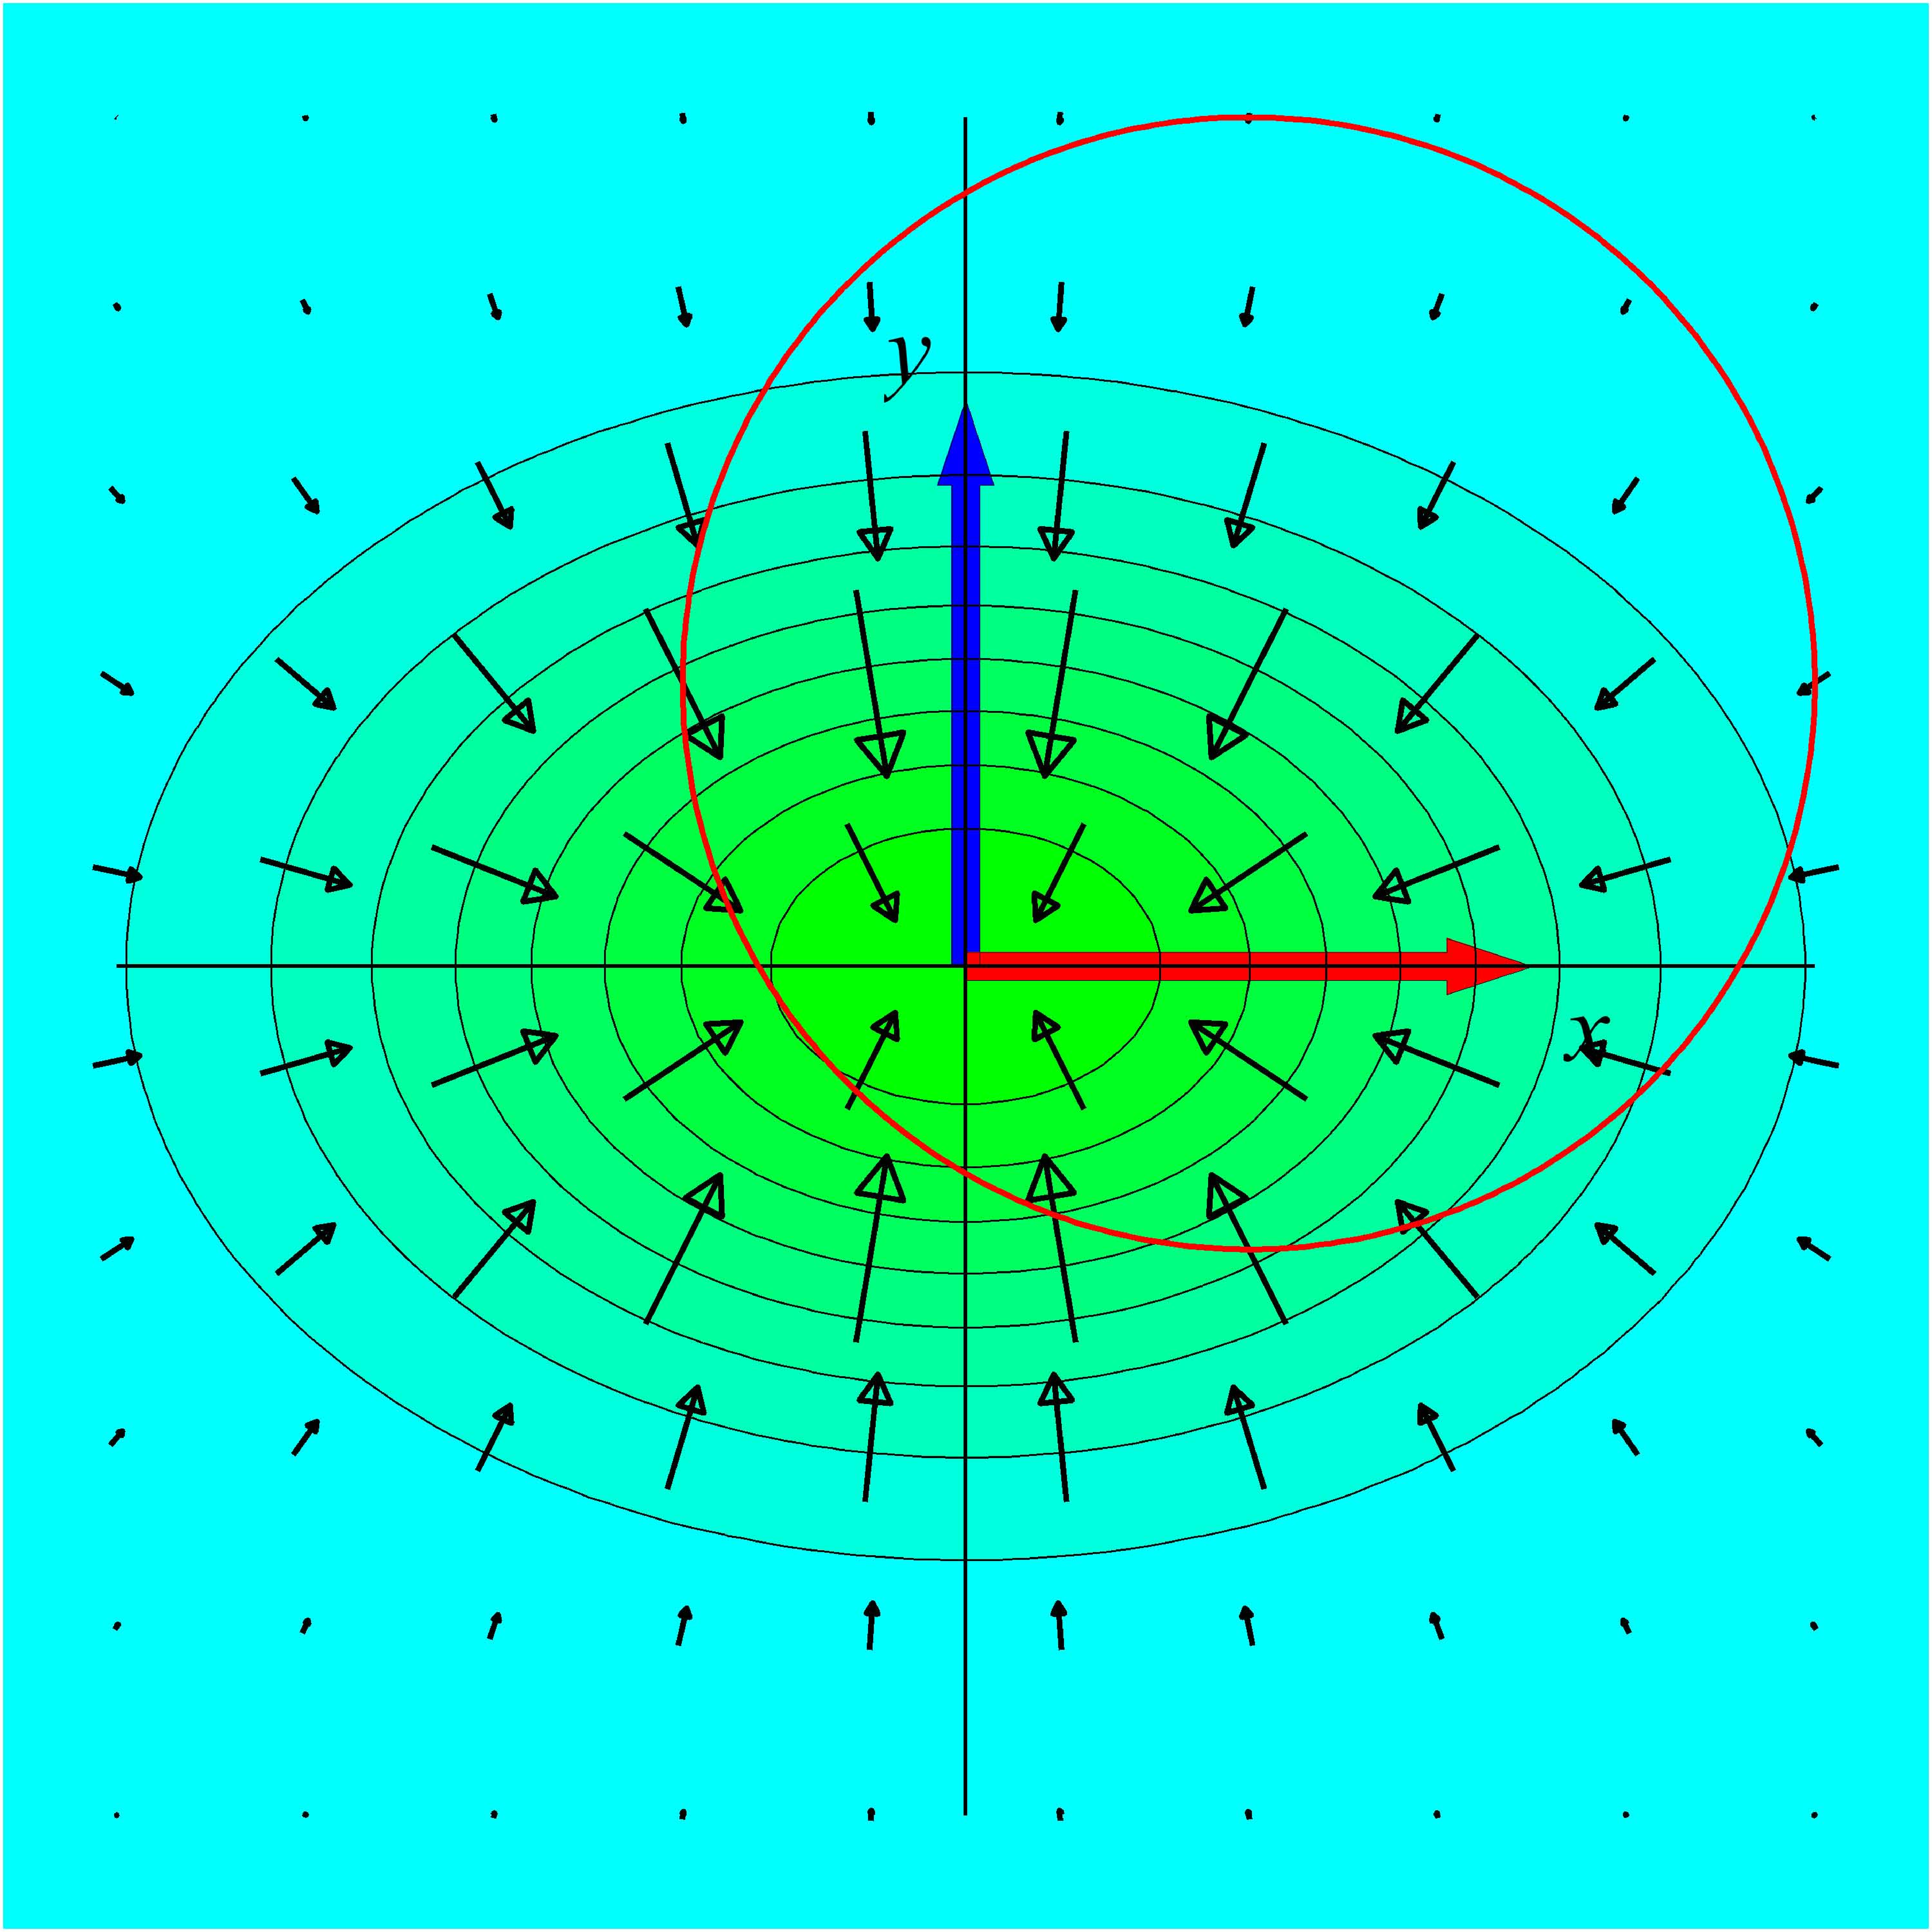
\includegraphics[height=75mm]{plotGradF.pdf}}
\begin{center}
\caption{Niveaukurver og gradientvektorfelt for funktionen $f(x,y) = 3 +  2\,\e^{-x^{2} - 2y^{2}}$.} \label{figMainFNivGrad}
\end{center}
\end{figure}

\begin{figure}[ht]
\centerline{ 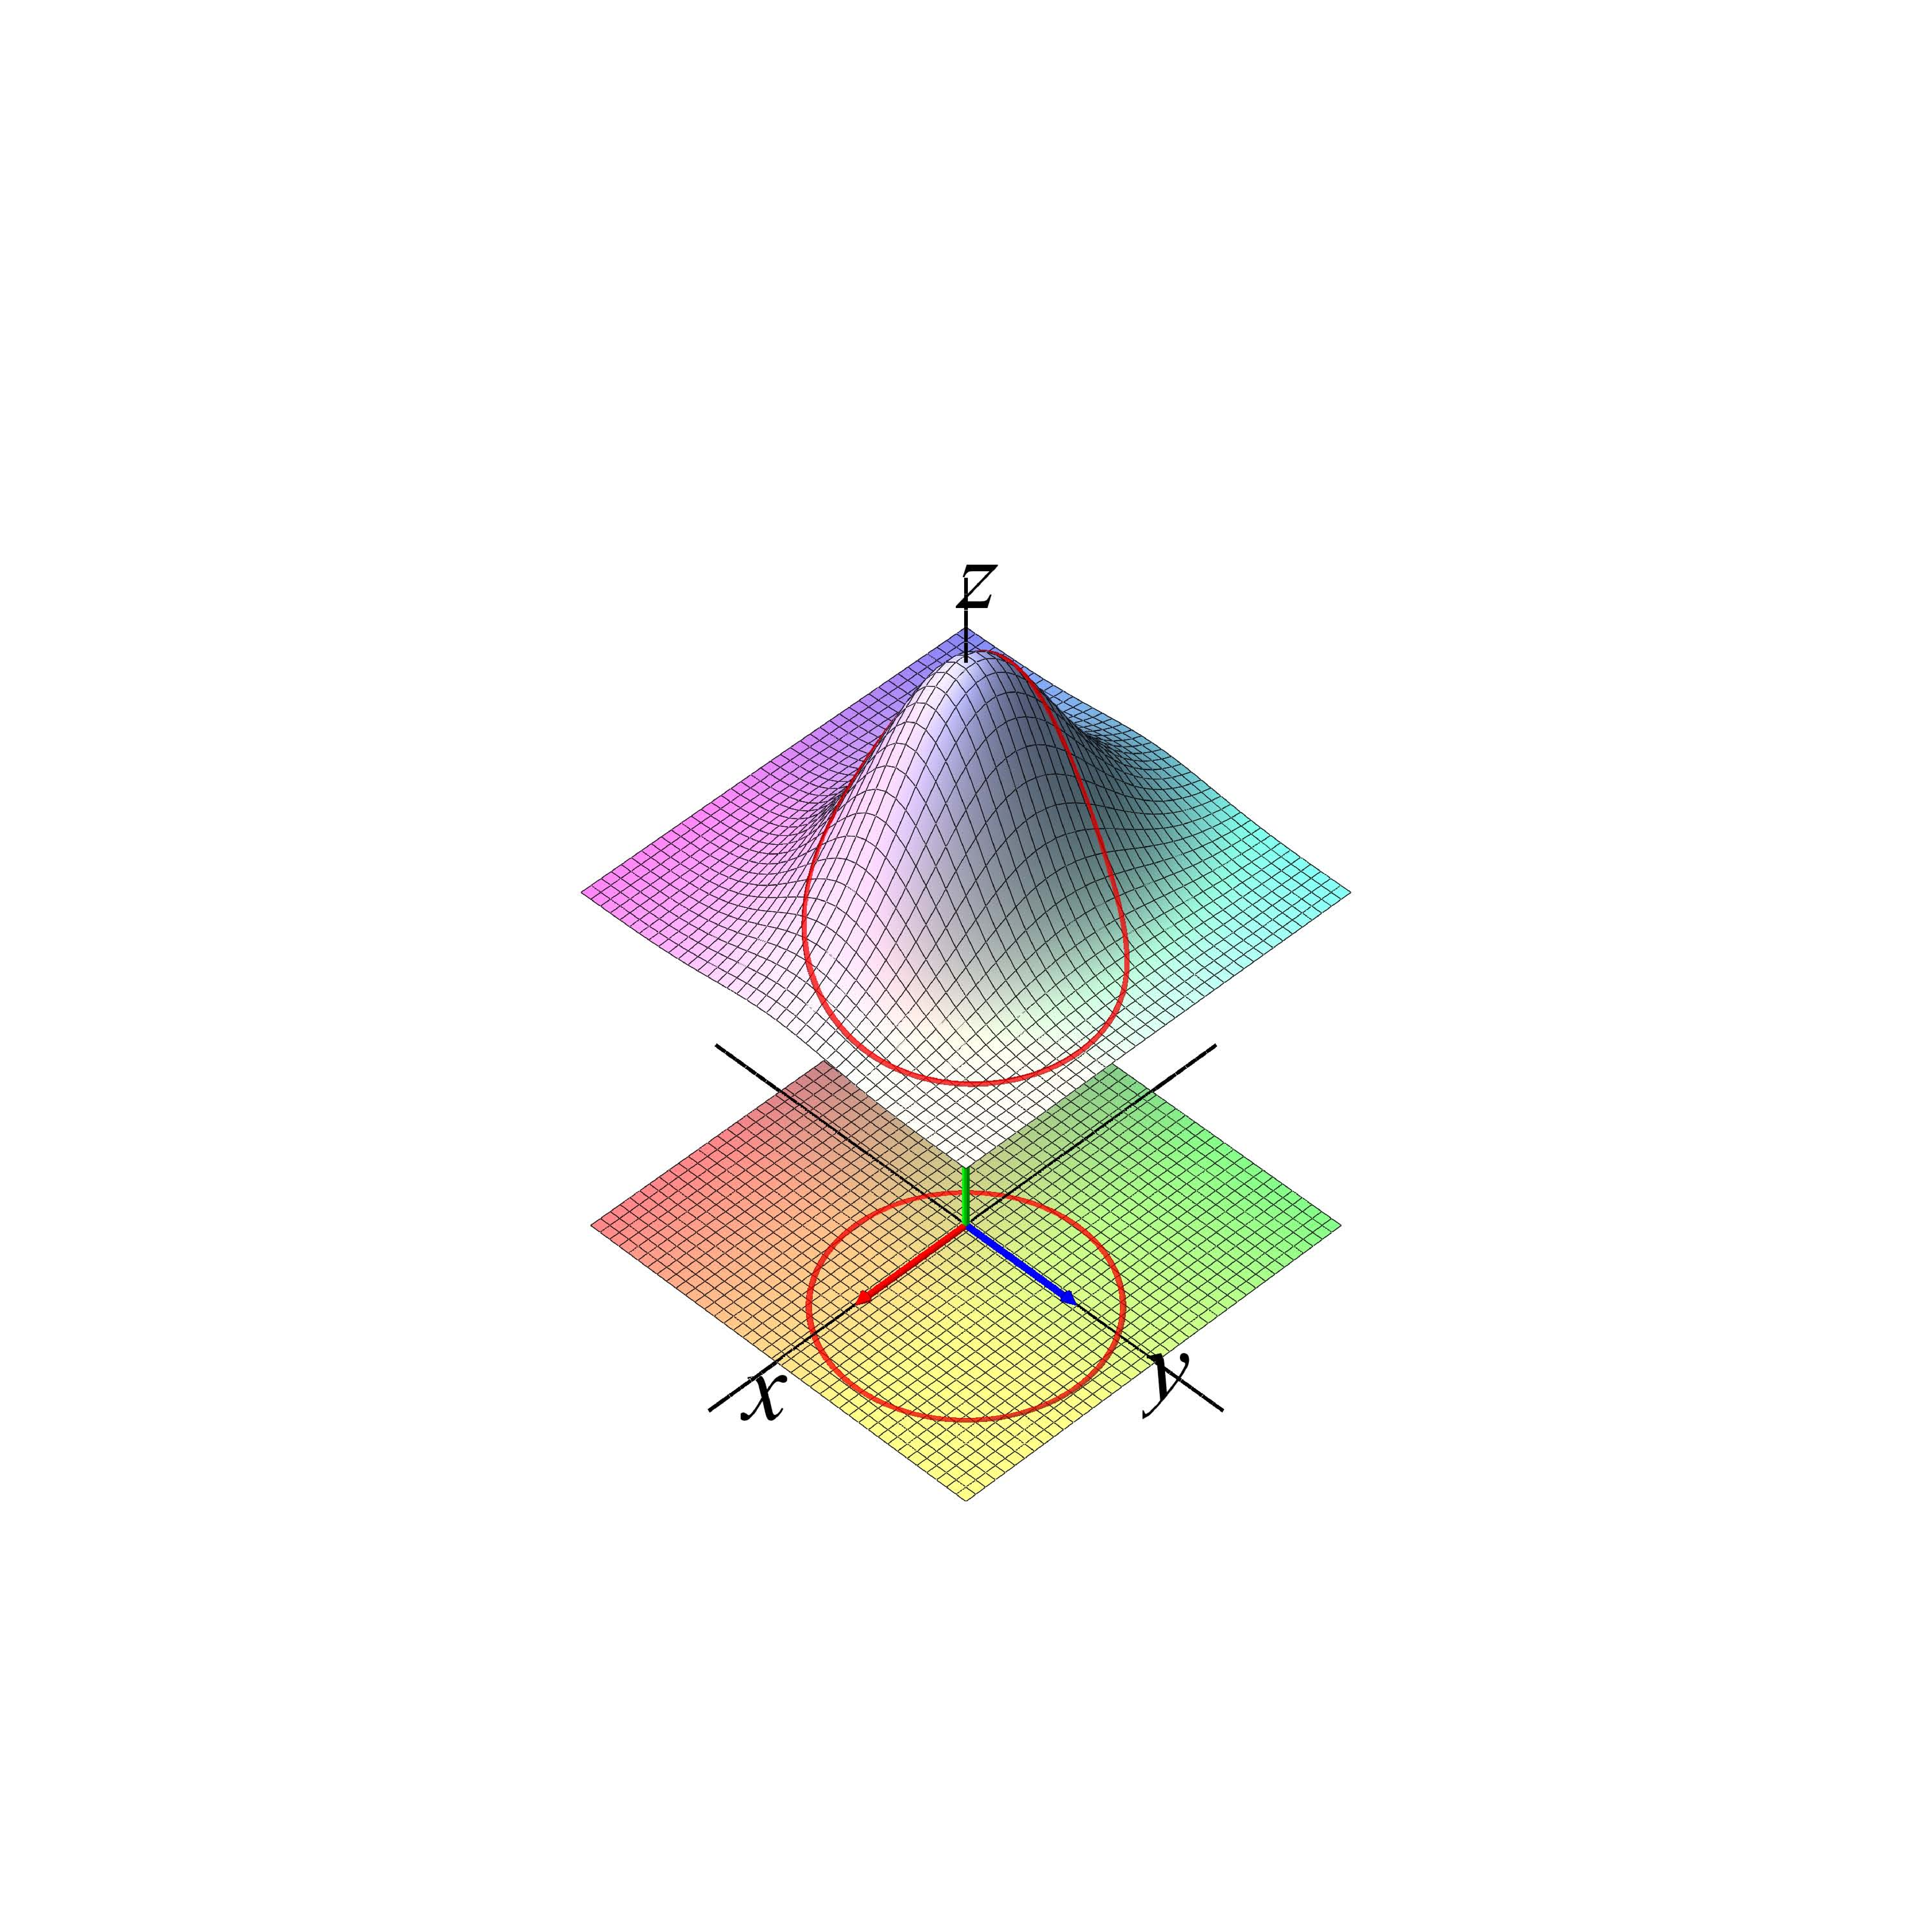
\includegraphics[height=95mm]{plotFigPureCurve01.pdf}}
\begin{center}
\caption{Grafen i $(x,y,z)$-rummet for $f(x,y) = 3 +  2\,\e^{-x^{2} - 2y^{2}}$.} \label{figMainF}
\end{center}
\end{figure}


\begin{exercise}
Bestem gradientvektorfelterne for følgende funktioner og skitser vektorfelterne ved at tegne et passende antal
af gradientvektorerne ${\bm{\nabla}}f(x_{0}, y_{0})$ med forskellige fodpunkter $(x_{0}, y_{0})$ i $(x,y)$-planen:
\begin{equation}
\begin{aligned}
  f(x,y) &= 3x + y \quad ,\\
  f(x,y) &= x^{2} + y^{2} \quad ,\\
  f(x,y) &= y\cdot\e^{x} \quad.
\end{aligned}
\end{equation}
\end{exercise}

\begin{think}
Hvis vi bevæger os på cirklen i $(x,y)$-planen i figur \ref{figMainFNivGrad} (for eksempel i positiv omløbsretning) og samtidig holder øje med hvilke niveau-kurver der krydses undervejs vil vi kunne afgøre, om vi bevæger os mod stigende eller faldende funktionsværdier -- dels ved at holde øje med farveskiftet og dels ved at se, om projektionen af gradientvektoren ind på bevægelsesretningen (den retningsafledede) er positiv eller negativ; hvis projektionen er positiv er vi på vej mod større funktionsværdier, hvis projektionen er negativ er vi på vej mod mindre funktionsværdier. Det samme kan naturligvis ses på grafen for funktionen, hvor det på ethvert sted på den løftede kurve er klart om vi er på vej opad eller nedad på graf-fladen.
\end{think}

\section{Løftede kurver på graf-flader}
Motiveret af graf-fladen med den løftede cirkel i figur \ref{figMainF} og motiveret af analysen i eksempel \ref{exampMainF} vil vi nu helt generelt definere og undersøge
løftede kurver:

\begin{definition}[Løftede kurver]
Vi lader $f(x,y)$ betegne en funktion af to variable og lader $\mathbf{r}(u)$ betegne en differentiabel parametriseret kurve  i $(x,y)$-planen:
\begin{equation}
\mathbf{r}(u) = (p(u), q(u)) \quad , \quad \textrm{hvor $u \in \, ]\alpha, \beta[ \quad ,$}
\end{equation}
og hvor $p(u)$ og $q(u)$ betegner to differentiable funktioner af \'{e}n variabel $u$.\\

Den \ind{løftede kurve}{løftede kurve} som hører til den plane kurve $\mathbf{r}(u)$ defineres til at være følgende kurve i $(x, y, z)$-rummet:
\begin{equation}
\widetilde{\mathcal{C}}_{\mathbf{r}}(f) \quad : \quad \widetilde{\mathbf{r}}(u) = (p(u), q(u), f(p(u), q(u))) \quad , \quad \textrm{hvor $u \in \, ]\alpha, \beta[ $} \quad .
\end{equation}
Den løftede kurve $\widetilde{\mathbf{r}}(u)$ er en rumlig kurve, som ligger på graf-fladen $\mathcal{G}(f)$ for funktionen $f(x,y)$.\\

Projektionen (lodret, langs $z$-aksen) af $\widetilde{\mathbf{r}}(u)$ på $(x,y)$-planen er naturligvis den plane kurve $\mathbf{r}(u)$.
\end{definition}

De løftede kurver $\widetilde{\mathbf{r}}(u)$ har tangentvektorer og tangentlinjer i rummet --  og de må jo afhænge dels af kurven  ${\mathbf{r}}(u)$ i $(x,y)$-planen og dels af funktionen $f(x,y)$. Følgende udtryk fås direkte ud fra kædereglen for funktionen $f(x,y)$ langs kurven $\mathbf{r}(u)$ -- dvs. kædereglen for den sammensatte funktion $h(u) = f(\mathbf{r}(u)) = f(p(u), q(u))$:

\begin{theorem}[Tangenter for løftede kurver]
Den $u$-afledede af den løftede kurve $\widetilde{\mathbf{r}}(u)$ er givet ved de $u$-afledede af de tre koordinatfunktioner:
\begin{equation}
\begin{aligned}
\widetilde{\mathbf{r}}\,'(u) &=  \left(p'(u), q'(u), \frac{d}{du}f(p(u), q(u)) \right) \\
&=  \left(p'(u), q'(u), h'(u) \right) \\
&= \left(p'(u), q'(u), {\bm{\nabla}}f(p(u), q(u))\bm{\cdot} (p'(u), q'(u)) \right) \quad.
\end{aligned}
\end{equation}
\emph{Tangenten} til den løftede kurve på graf-fladen for $f(x,y)$ er derfor bestemt ved følgende udtryk i et givet kurvepunkt $\widetilde{\mathbf{r}}(u_{0}) = (p(u_{0}), q(u_{0}), f(p(u_{0}), q(u_{0})) = (x_{0}, y_{0}, f(x_{0}, y_{0}))$:
\begin{equation} \label{eqTangLift}
\begin{aligned}
\widetilde{L}_{u_{0}} \, \,  : \, \,  \widetilde{\mathbf{T}}(t) &=\widetilde{\mathbf{r}}(u_{0}) + t\cdot \widetilde{\mathbf{r}}\,'(u_{0}) \\
&= (x_{0}, y_{0}, f(x_{0}, y_{0})) + \\
& \qquad t\cdot \left(p'(u_{0}), q'(u_{0}), {\bm{\nabla}}f(x_{0}, y_{0})\bm{\cdot} (p'(u_{0}), q'(u_{0})) \right) \, \, ,
\end{aligned}
\end{equation}
hvor parameteren $t$ gennemløber hele $\mathbb{R}$.
\end{theorem}


\subsection{Løftede koordinat-kurver} \label{subsecLift}
Koordinatkurverne i $(x,y)$-planen er de   særligt simple kurver (rette linjer), som er parallelle med koordinatakserne. Igennem punktet $(x_{0}, y_{0})$ har vi følgende to:
\begin{equation}
\begin{aligned}
\mathbf{r}_{1}(u) &= (u, y_{0}) \quad \textrm{hvor $u \in \mathbb{R}$}\quad , \\
\mathbf{r}_{2}(u) &= (x_{0}, u) \quad \textrm{hvor $u \in \mathbb{R}$} \quad .
\end{aligned}
\end{equation}
De har derfor også særligt simple løft til graf-fladen for en given funktion $f(x,y)$:
\begin{equation}
\begin{aligned}
\widetilde{\mathbf{r}}_{1}(u) &= (u, y_{0}, f(u, y_{0})) \quad, \quad \textrm{$u \in \mathbb{R}$}\quad , \\
\widetilde{\mathbf{r}}_{2}(u) &= (x_{0}, u, f(x_{0}, u))\quad, \quad  \textrm{$u \in \mathbb{R}$} \quad ,
\end{aligned}
\end{equation}
med særligt simple $u$-afledede for ethvert $u$:
\begin{equation}
\begin{aligned}
\widetilde{\mathbf{r}}\,'_{1}(u) &= (1, 0, f'_{x}(u, y_{0}))\quad, \quad  \textrm{$u \in \mathbb{R}$}\quad , \\
\widetilde{\mathbf{r}}\,'_{2}(u) &= (0, 1, f'_{y}(x_{0}, u)) \quad, \quad \textrm{$u \in \mathbb{R}$}\quad .
\end{aligned}
\end{equation}

Tangenterne i punktet $(x_{0}, y_{0}, f(x_{0}, y_{0}))$ til de løftede koordinatkurver er derfor også rimeligt simple:
\begin{equation}
\begin{aligned}
\widetilde{L}_{1} \quad : \quad (x_{0}, y_{0}, f(x_{0}, y_{0})) + t\cdot(1, 0, f'_{x}(x_{0}, y_{0})) \quad , \quad \textrm{$t \in \mathbb{R}$} \\
\widetilde{L}_{2} \quad : \quad(x_{0}, y_{0}, f(x_{0}, y_{0})) + t\cdot(0, 1, f'_{y}(x_{0}, y_{0}))  \quad , \quad \textrm{$t \in \mathbb{R}$}
\end{aligned}
\end{equation}


\begin{exercise}
Bestem (for ethvert punkt $(x_{0},y_{0})$ i $(x,y)$-planen) tangenterne til de løftede koordinatkurver igennem graf-fladepunktet $(x_{0}, y_{0}, f(x_{0}, y_{0}))$ for funktionerne:
\begin{equation}
\begin{aligned}
  f(x,y) &= 3x + y \quad ,\\
  f(x,y) &= x^{2} + y^{2}\quad , \\
  f(x,y) &= y\cdot\e^{x} \quad.
\end{aligned}
\end{equation}
\end{exercise}



I figurerne \ref{figMainFDiverse} ses den løftede cirkel og graf-fladen for funktionen $f(x,y)$ fra eksempel \ref{exampMainF}. Den løftede kurves tangenter er indtegnet i et par udvalgte punkter.
Bemærk, at de rumlige tangenter til den løftede kurve projicerer ned på de tilsvarende tangenter til cirklen i $(x,y)$-planen -- som det også følger af ligning (\ref{eqTangLift}).



\begin{figure}[ht]
\centerline{ 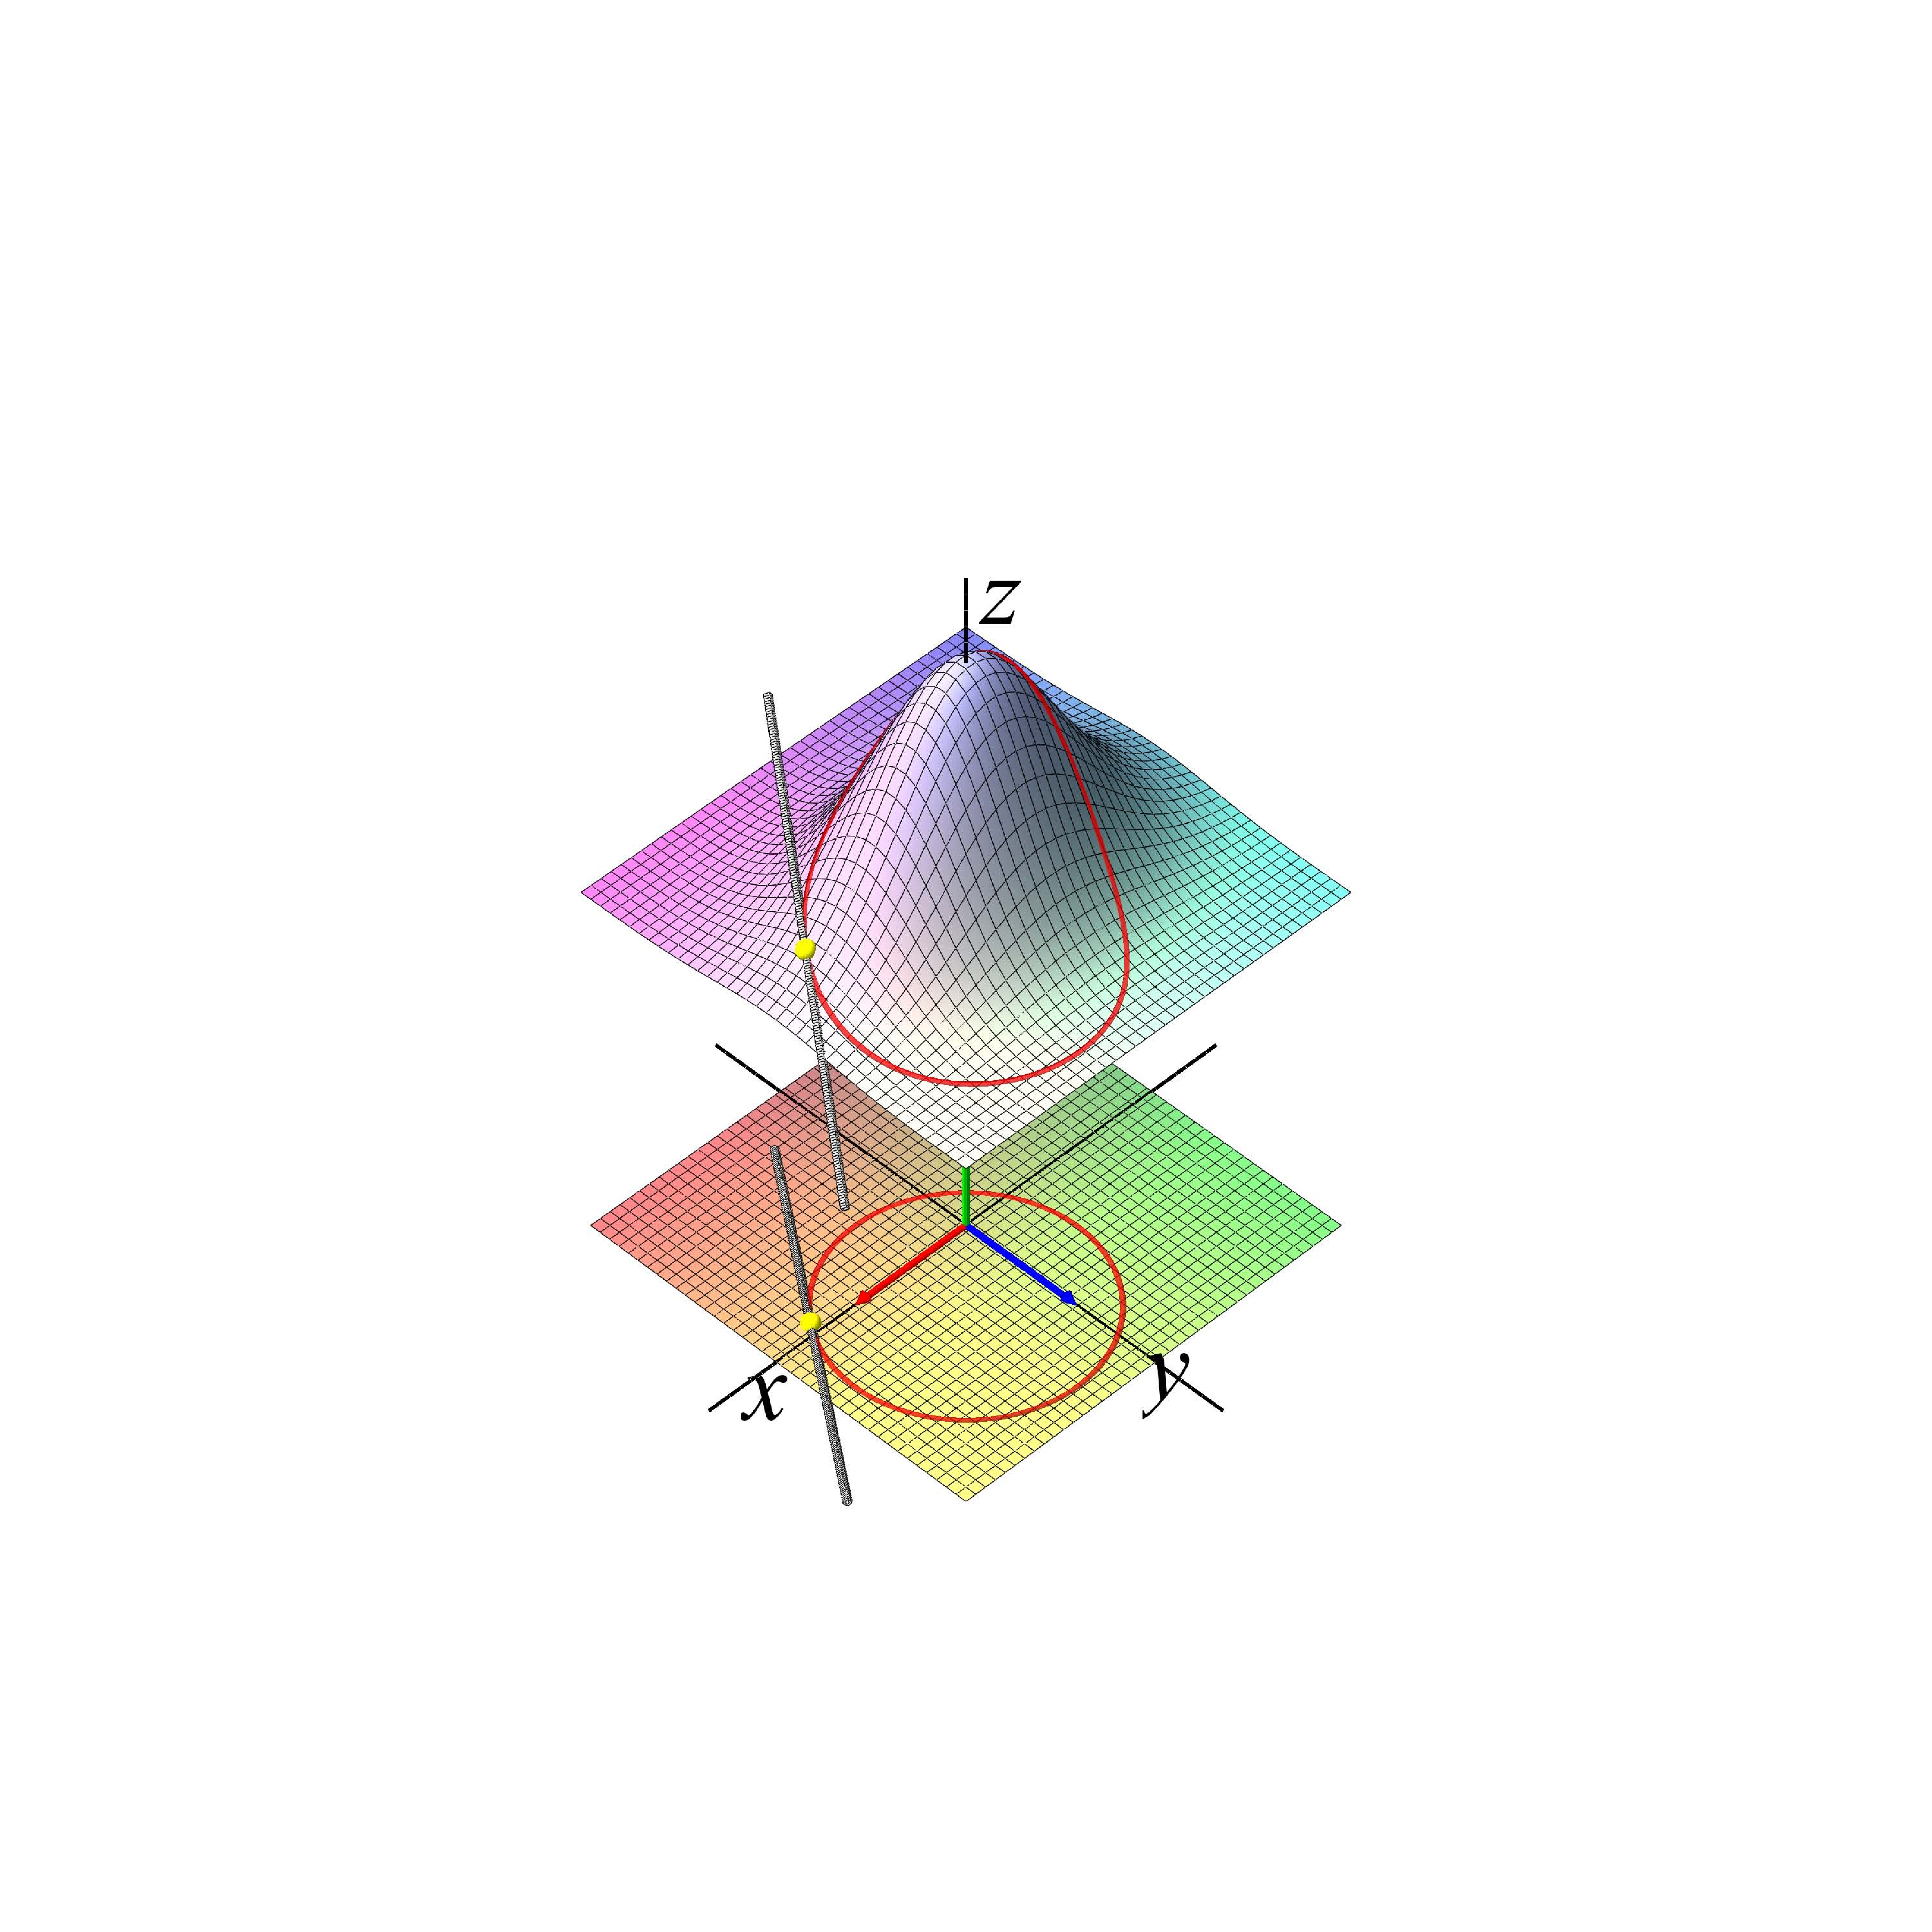
\includegraphics[height=75mm]{plotTang02negB.pdf} 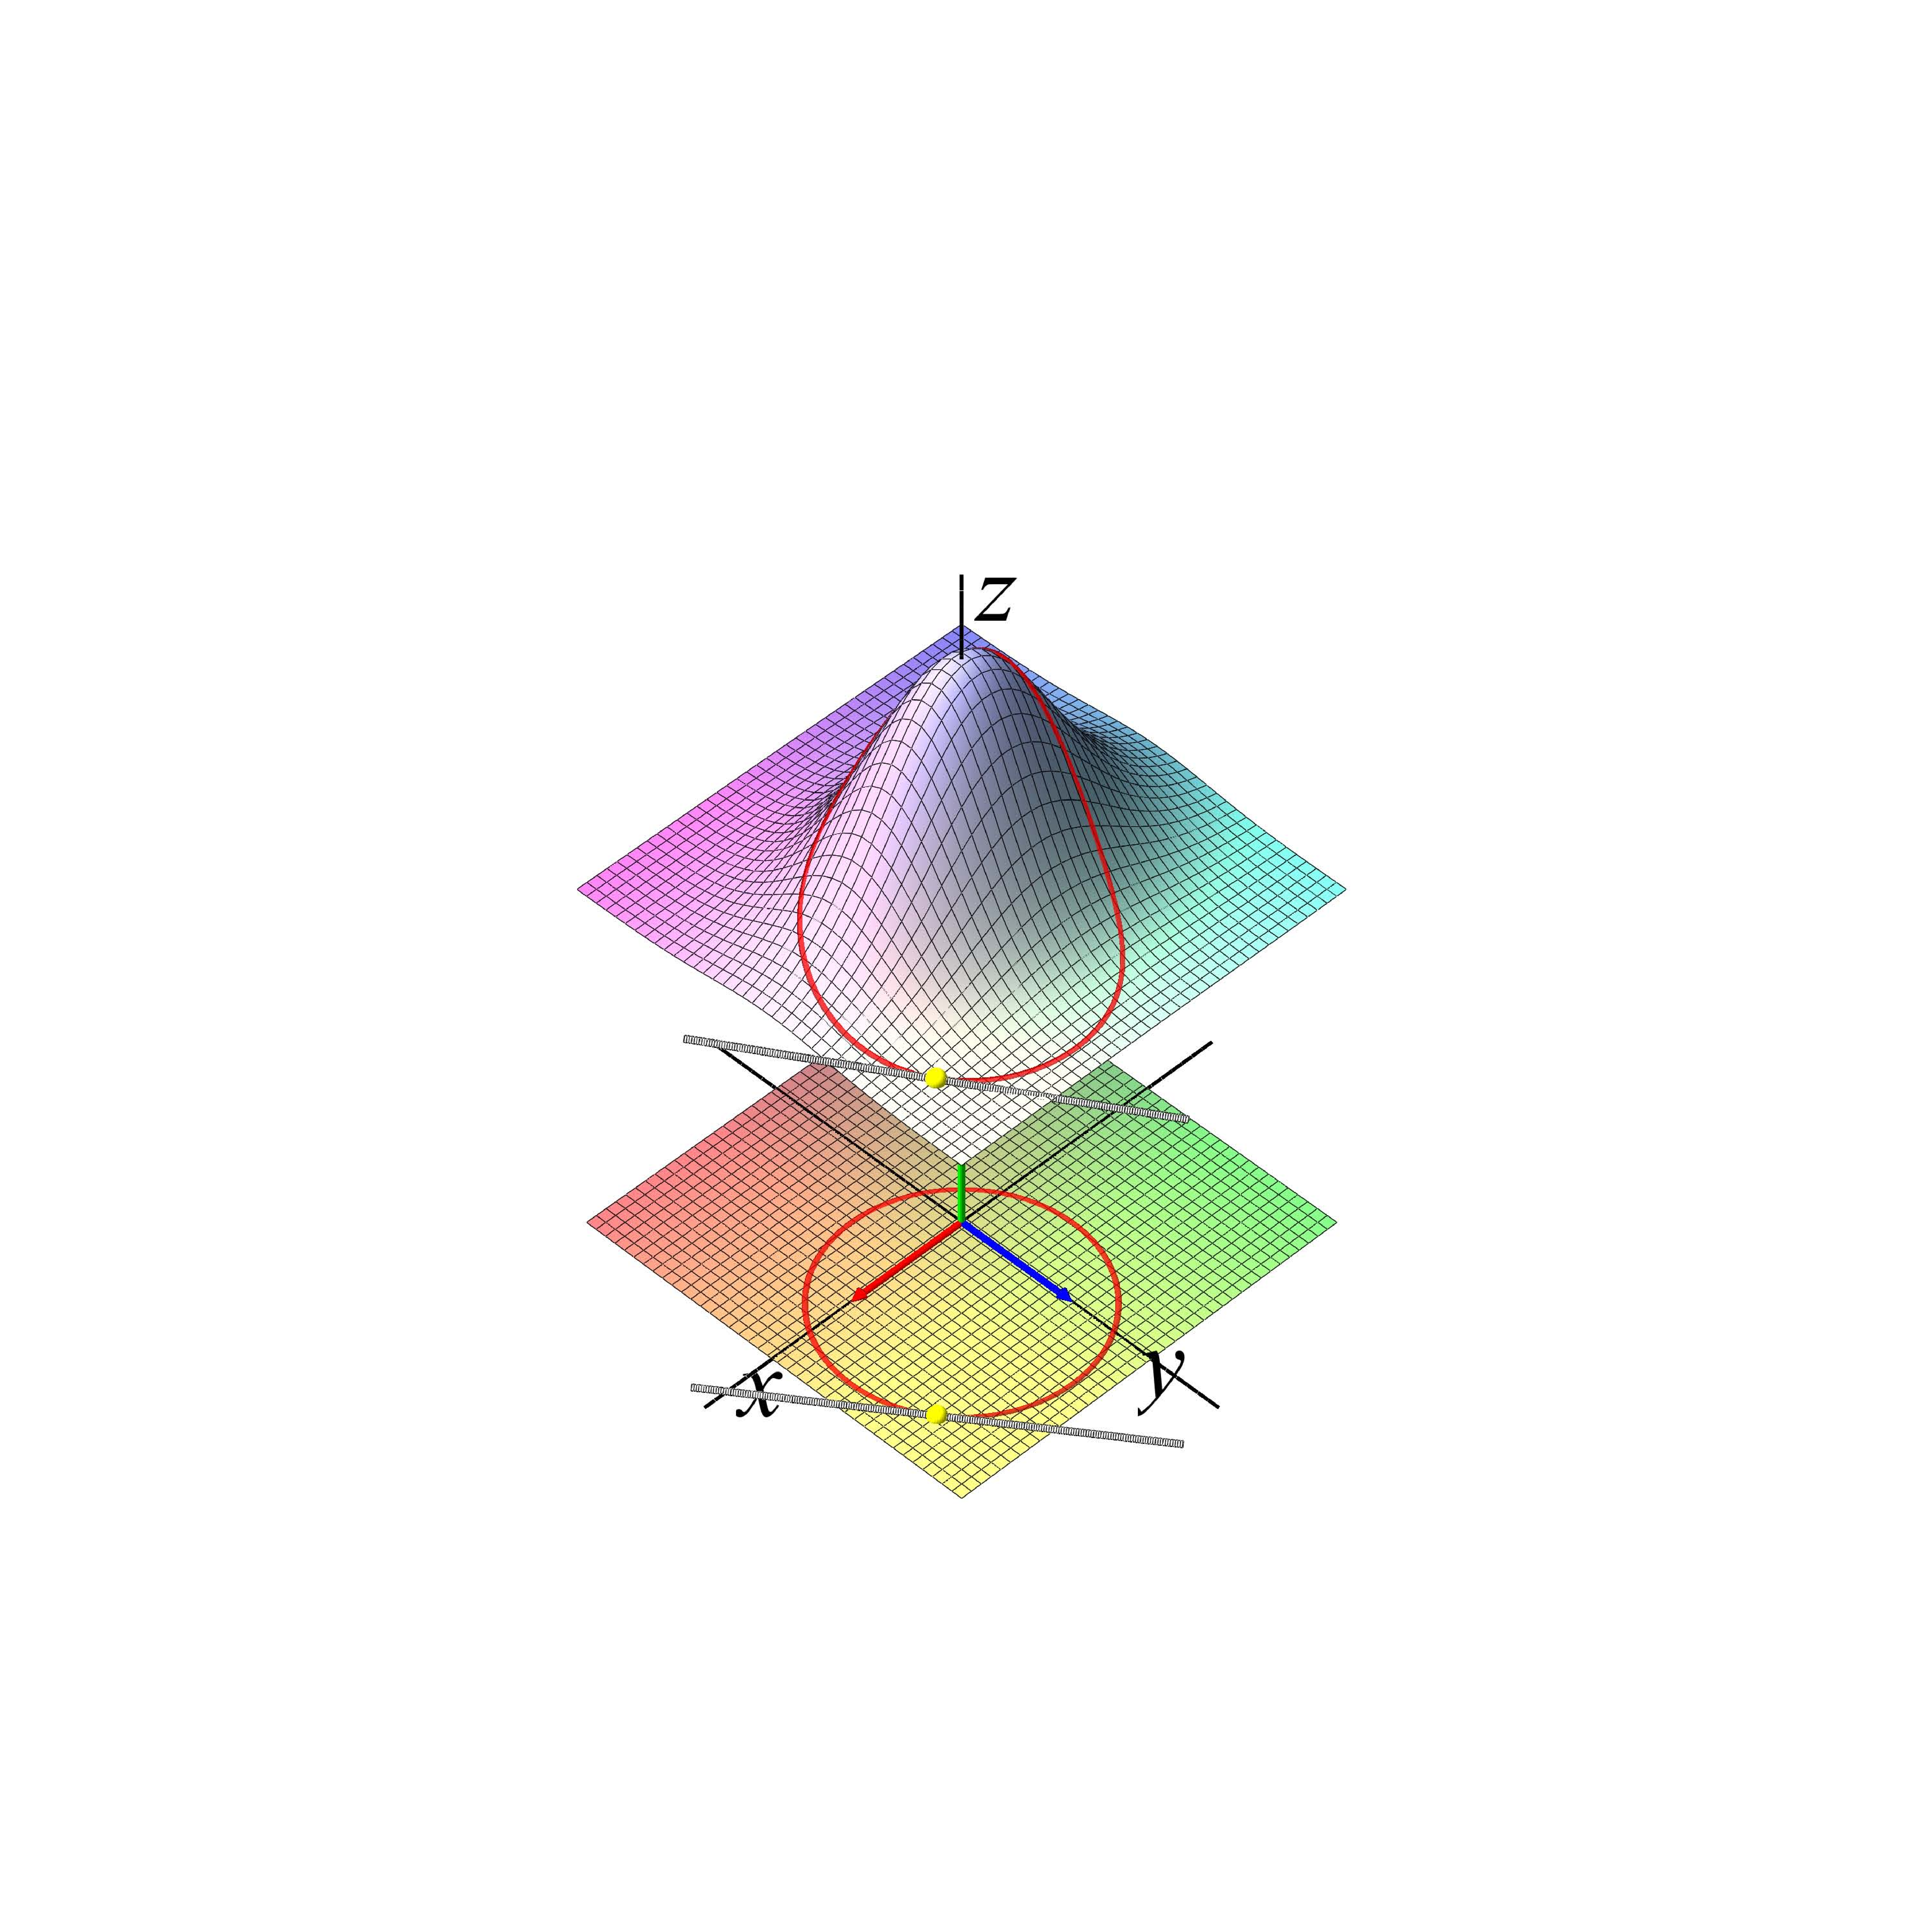
\includegraphics[height=75mm]{plotTang02B.pdf} 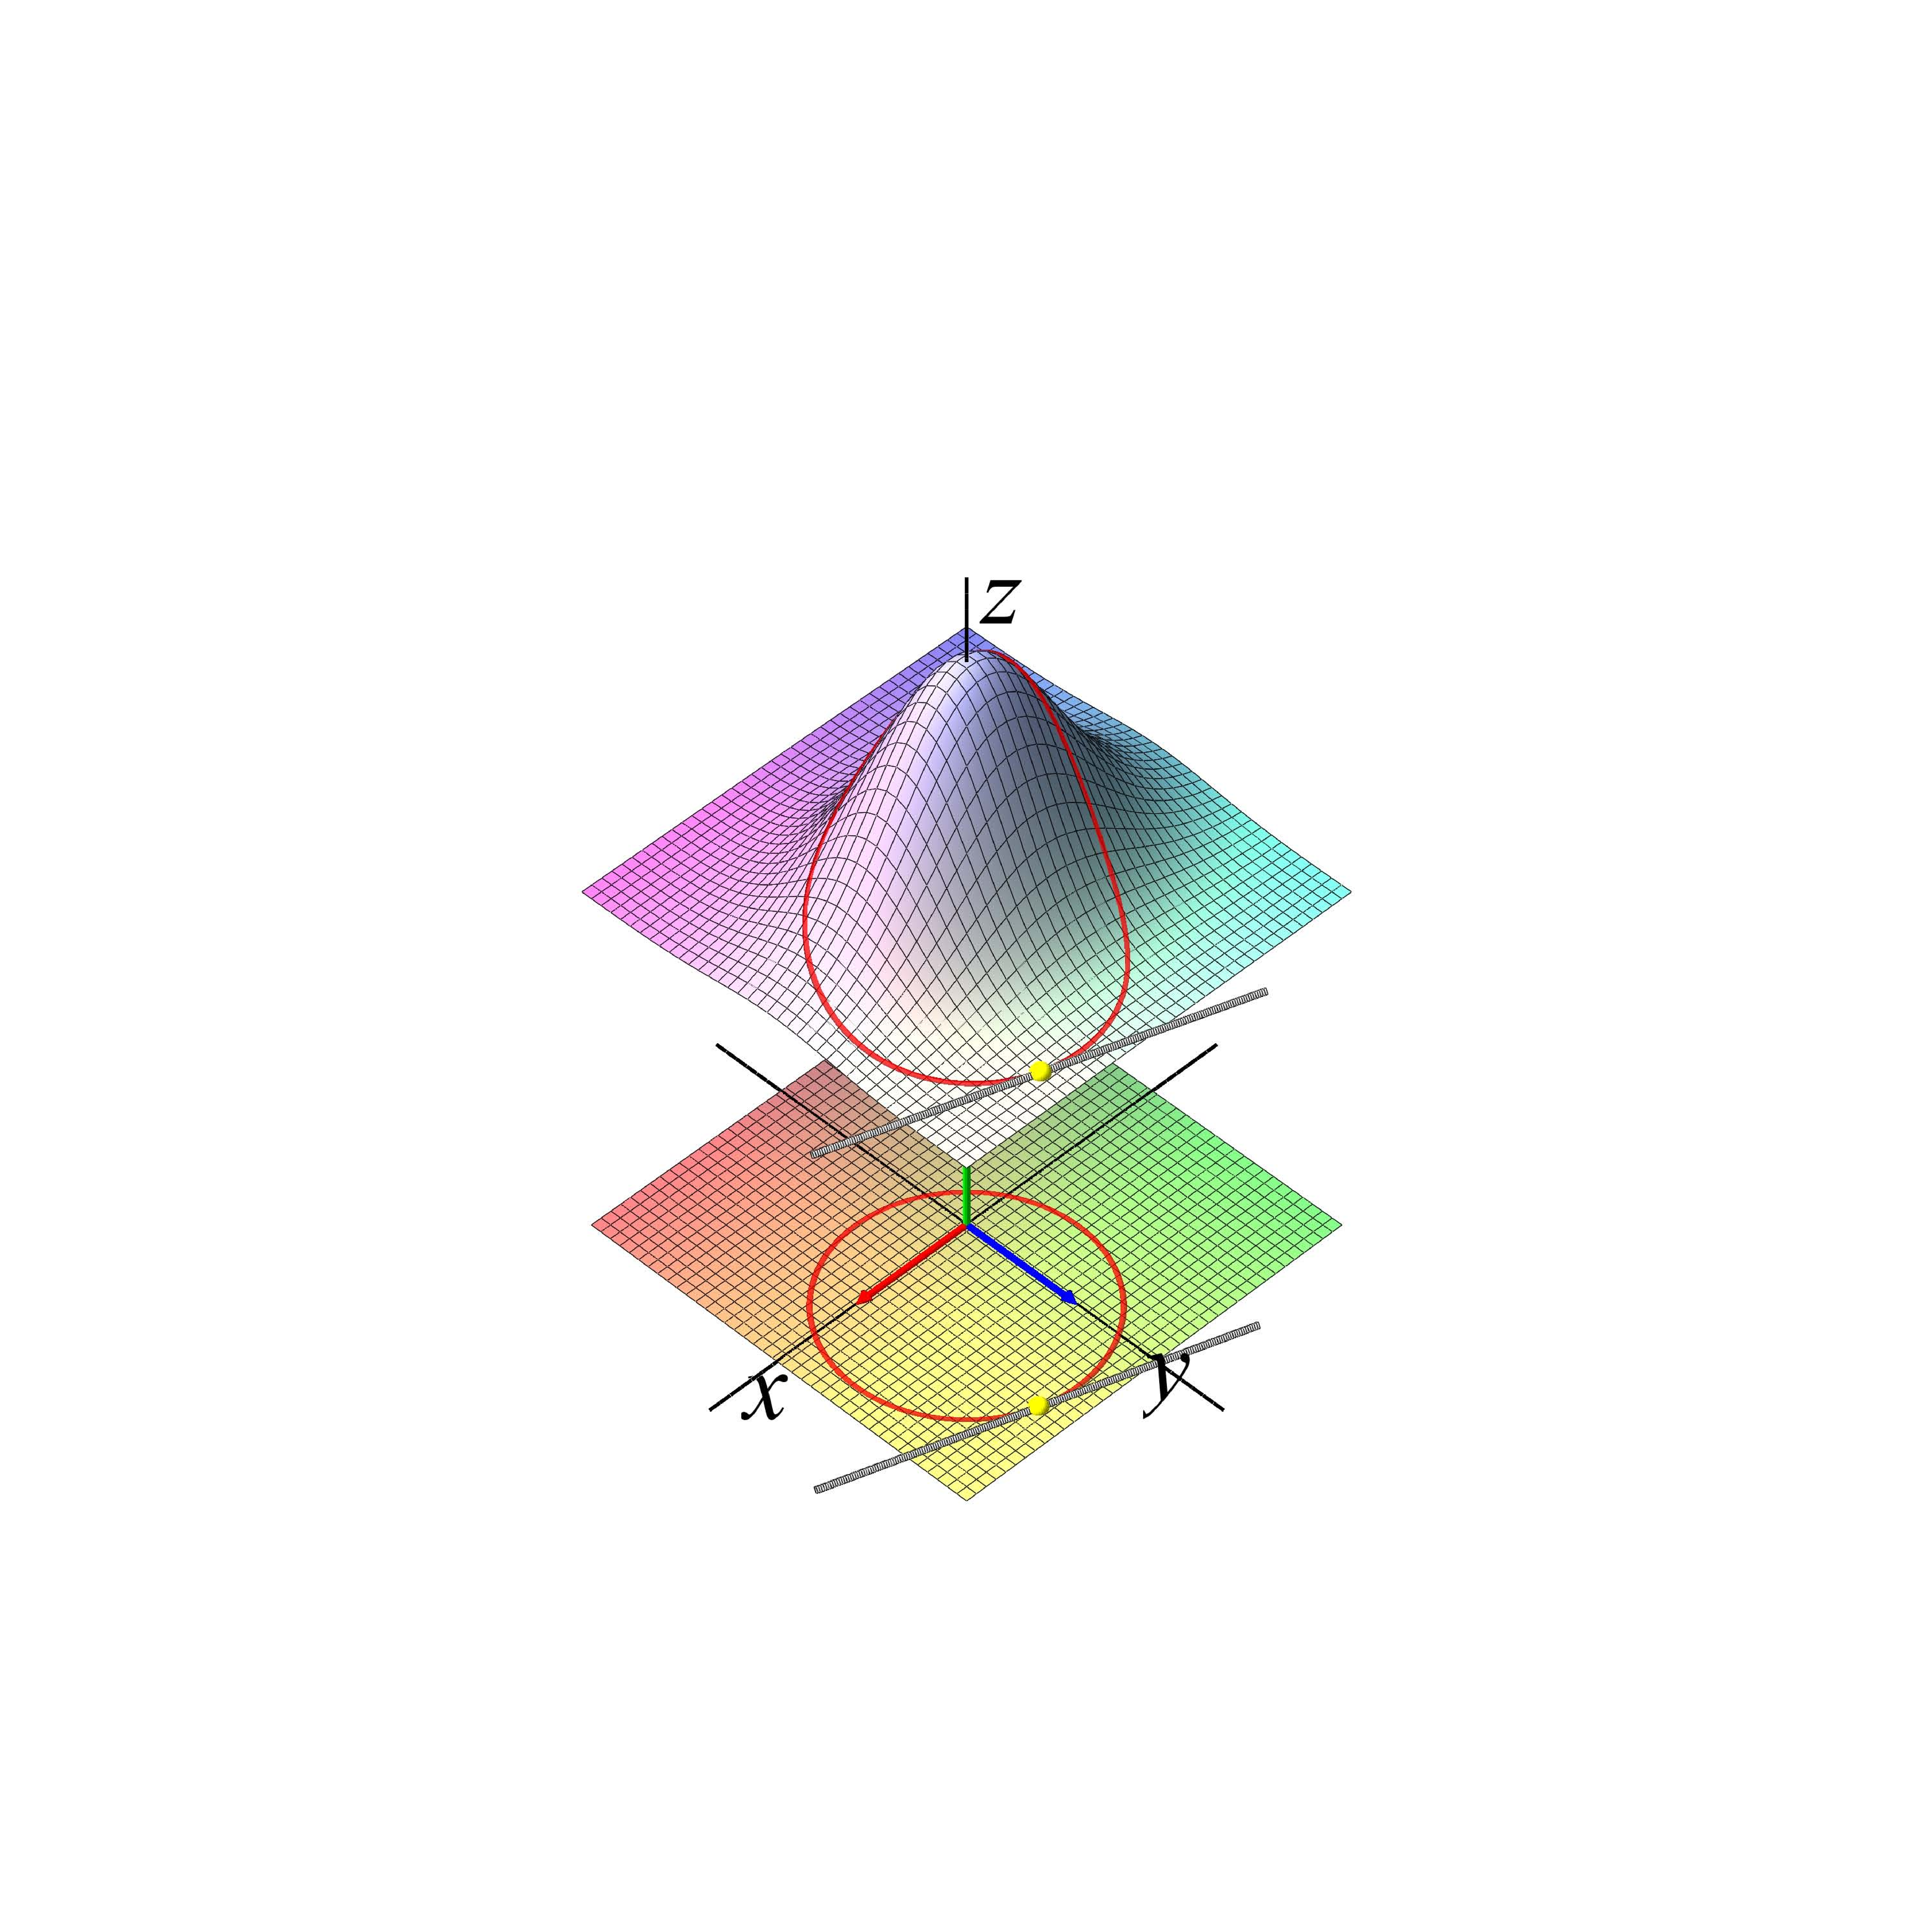
\includegraphics[height=75mm]{plotTang04B.pdf}}
\begin{center}
\caption{Grafen for $f(x,y) = 3 +  2\,\e^{-x^{2} - 2y^{2}}$ med udvalgte tangenter til en løftet cirkel.} \label{figMainFDiverse}
\end{center}
\end{figure}




\begin{aha}
Graf-fladens tangentplan i et givet punkt $(x_{0}, y_{0}, f(x_{0}, y_{0}))$ er jo selv graf-fladen for det approksimerende første-gradspolynomium for $f(x,y)$ med udviklingspunktet $(x_{0},y_{0})$ og er derfor uafhængig af hvilken kurve vi måtte finde på at løfte op på graf-fladen igennem punktet $(x_{0}, y_{0}, f(x_{0}, y_{0}))$! Ikke desto mindre ser det i figurerne ud til, at \emph{kurvens tangenter} ligger helt indeholdt i de respektive tangentplaner. \\

Den inspektion giver derfor anledning til følgende formodning, som vi vil vise rigtigheden af i sætning \ref{thmTangentTangent} nedenfor: Enhver tangent til enhver løftet kurve igennem et givet punkt $(x_{0}, y_{0}, f(x_{0}, y_{0}))$ ligger i tangentfladen for $f(x, y)$ i punktet. Og omvendt: Enhver ret linje i tangentplanen som går igennem punktet  $(x_{0}, y_{0}, f(x_{0}, y_{0}))$ er tangent til en eller anden løftet kurve som går igennem punktet.
\end{aha}

\begin{figure}[ht]
\centerline{ 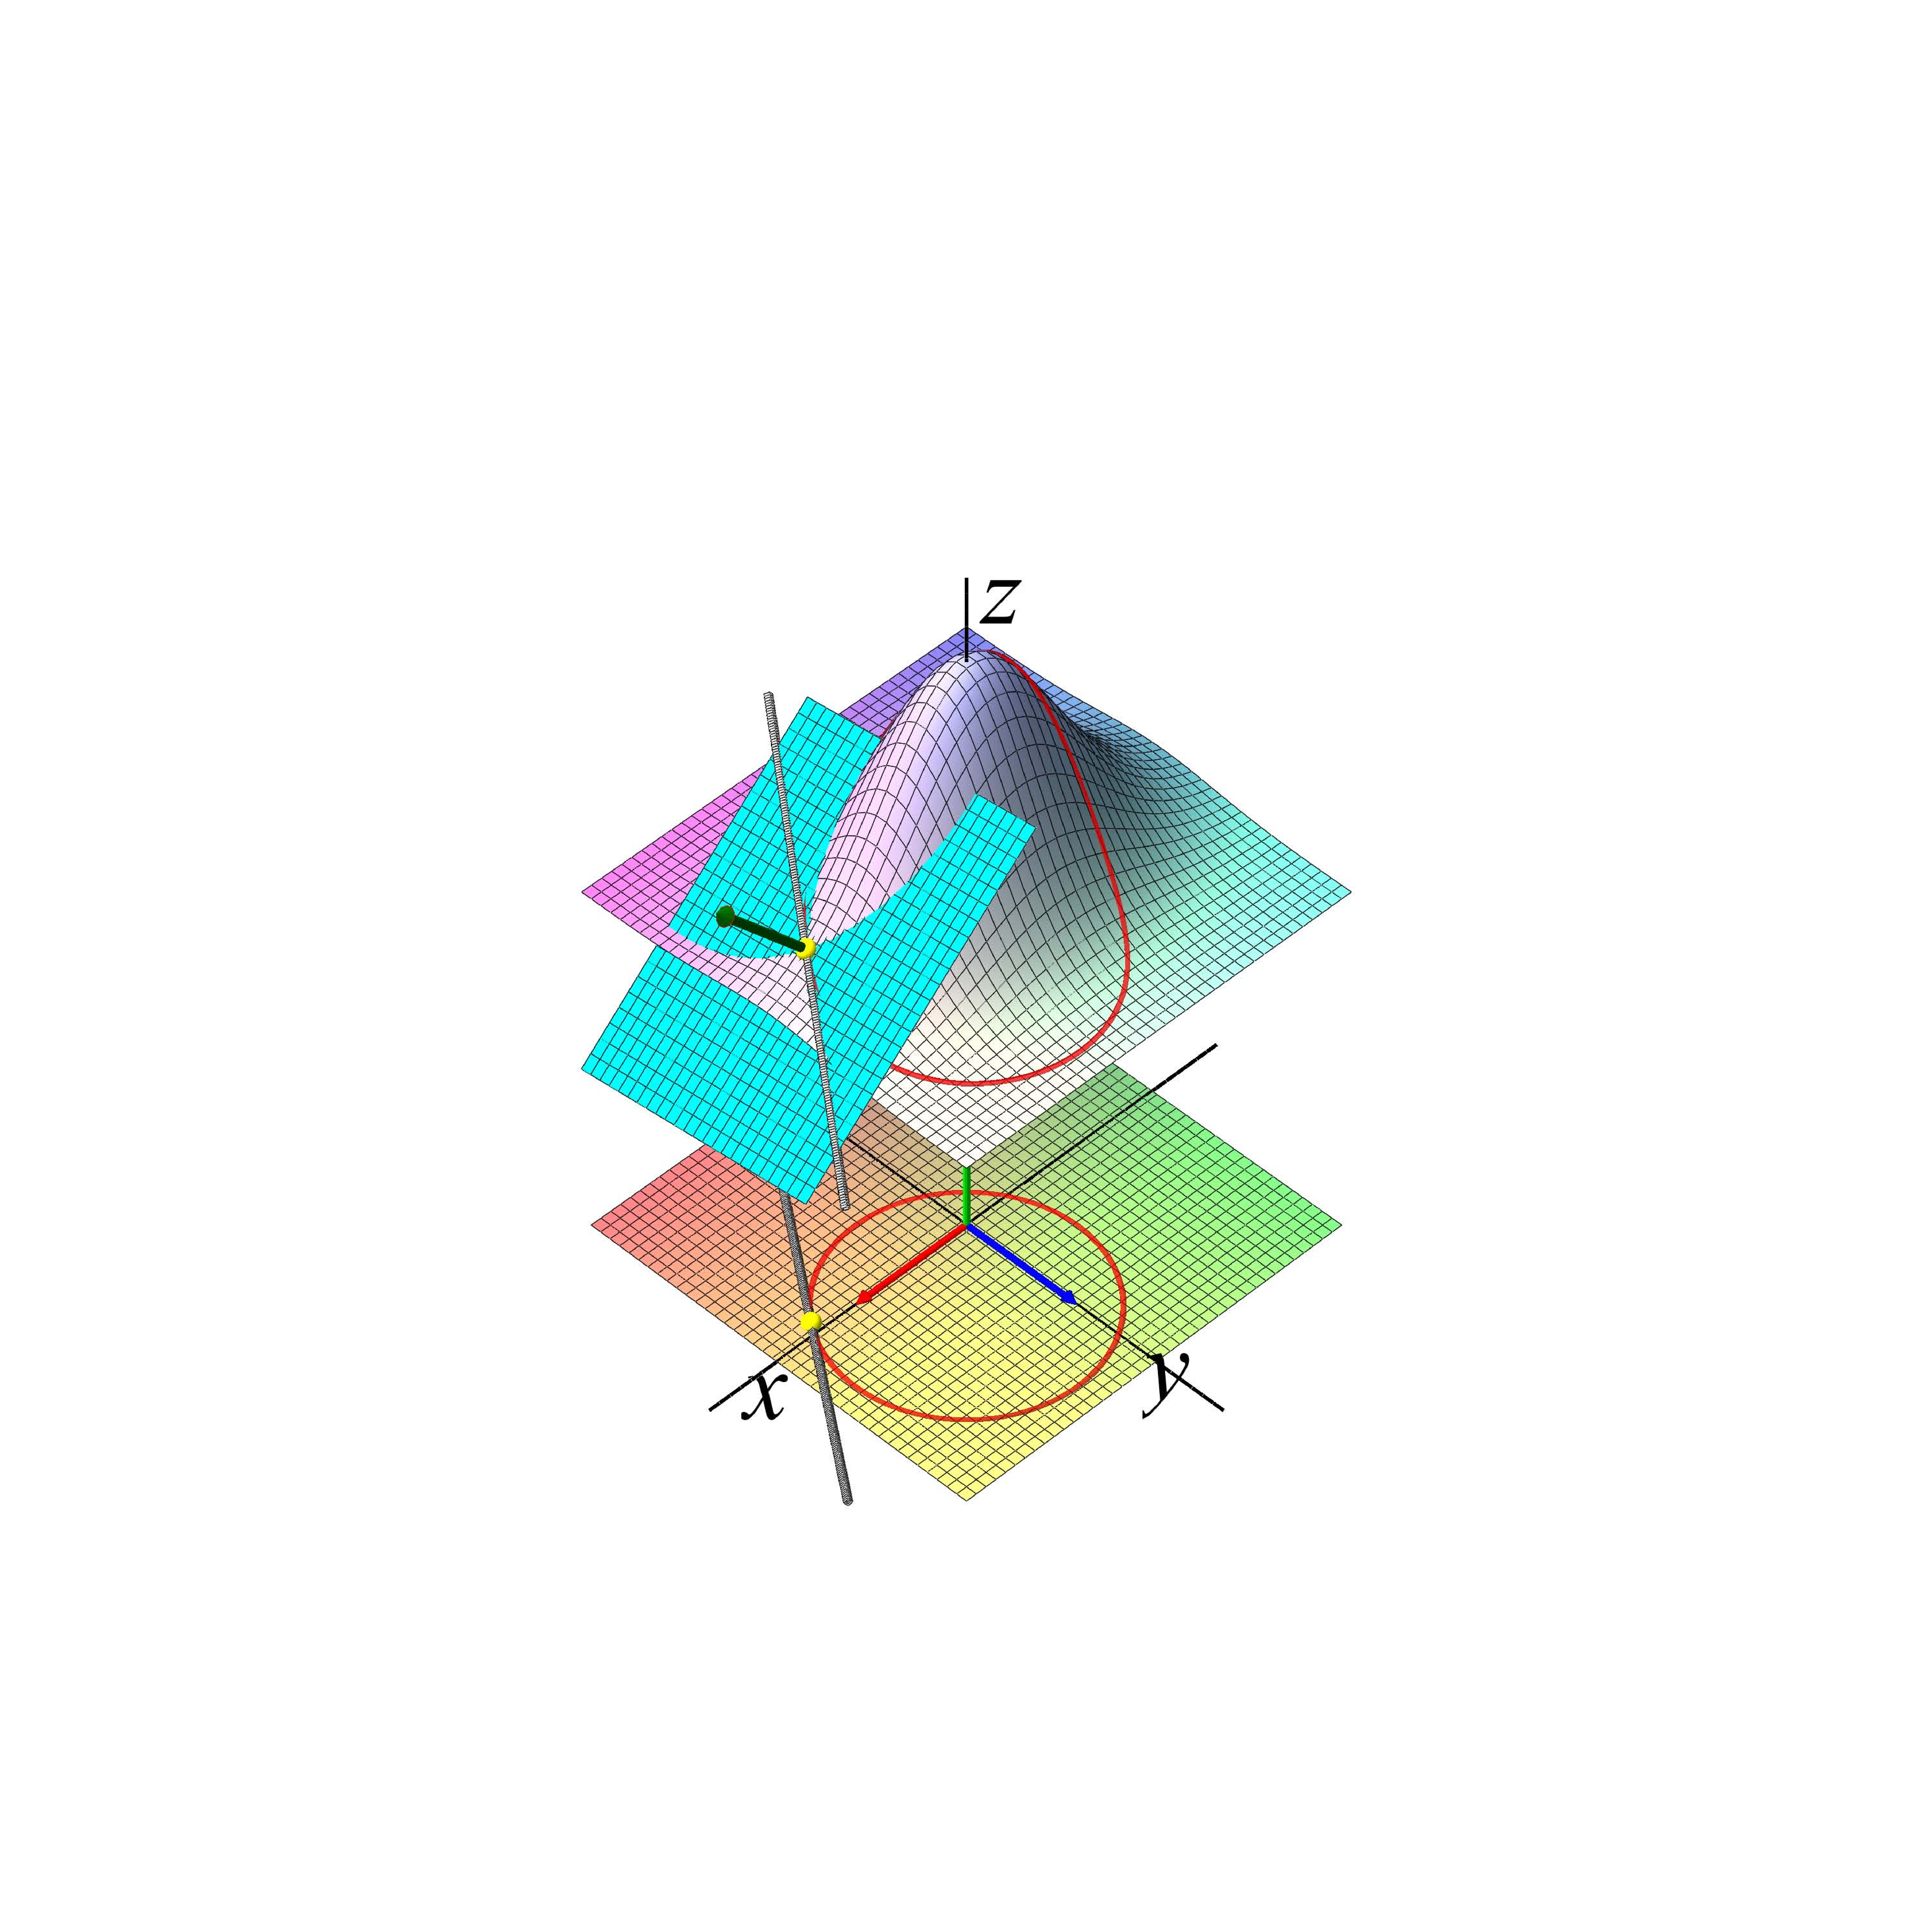
\includegraphics[height=105mm]{plotTangFull02Bneg.pdf}}
\begin{center}
\caption{Grafen for $f(x,y) = 3 +  2\,\e^{-x^{2} - 2y^{2}}$ og tangentplanen igennem et udvalgt punkt på den løftede cirkel, se figur \ref{figMainF}.} \label{figMainFTplanerA}
\end{center}
\end{figure}

\begin{figure}[ht]
\centerline{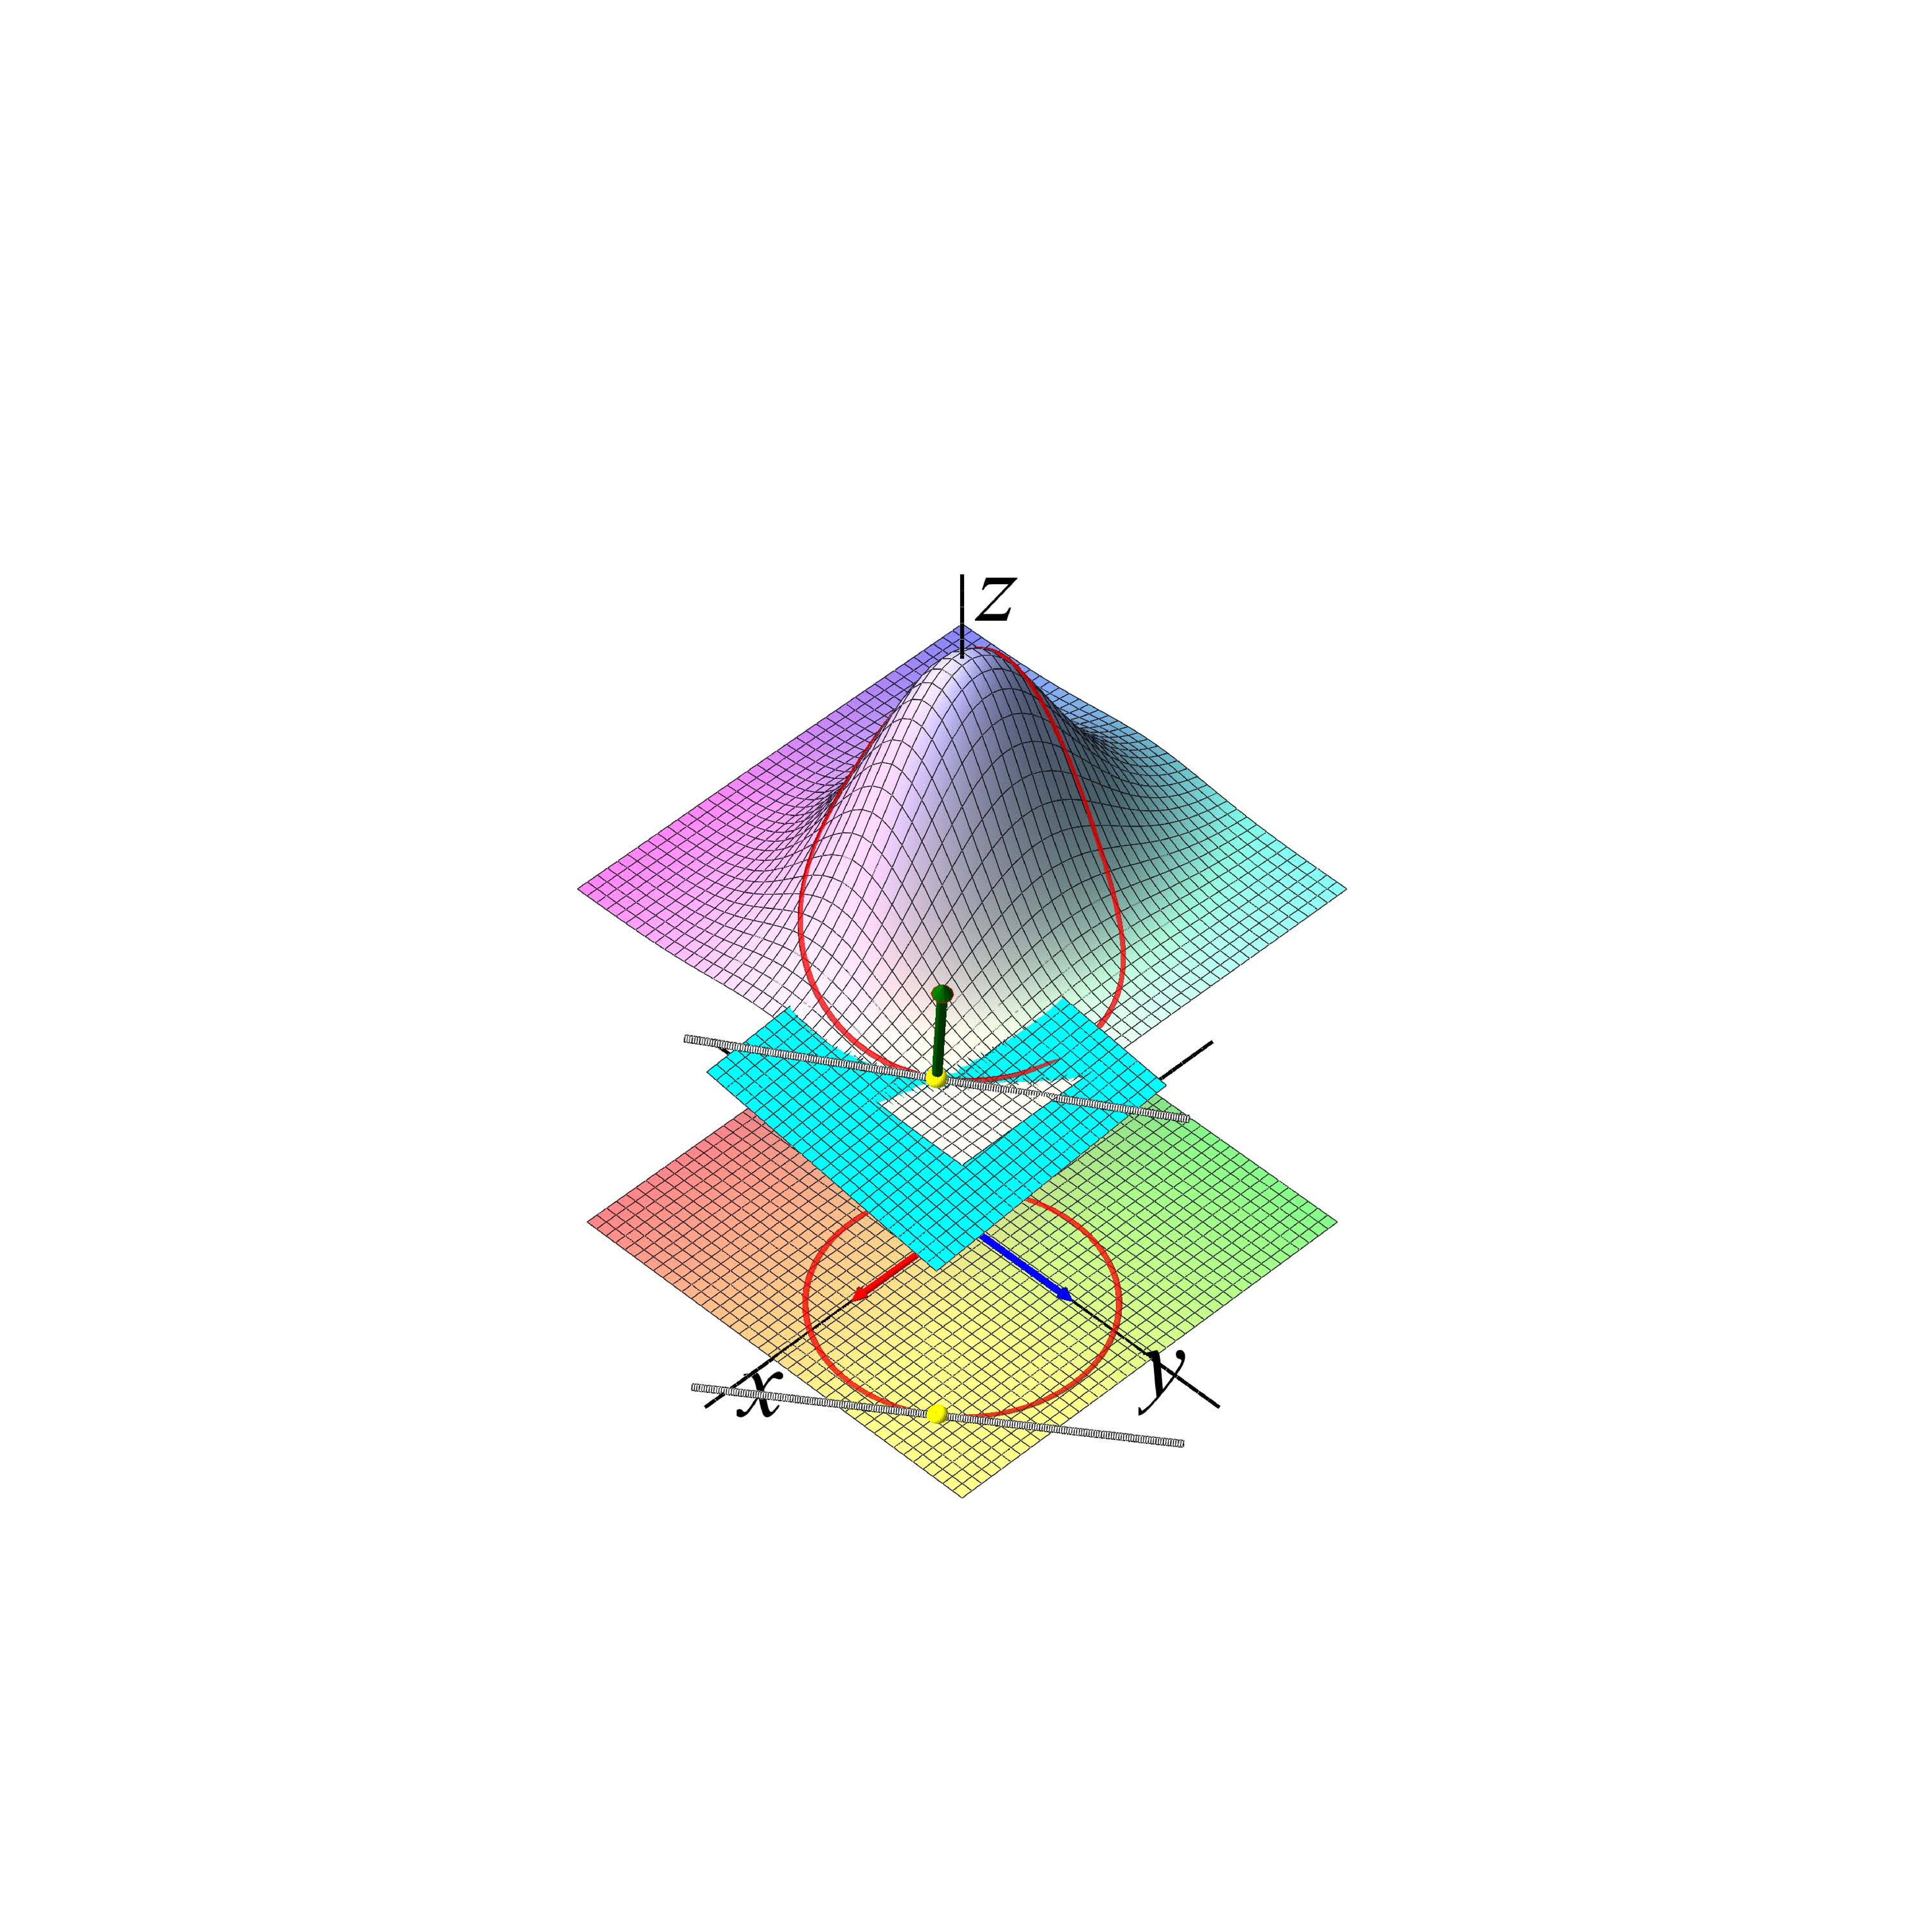
\includegraphics[height=105mm]{plotTangFull02B.pdf} }
\begin{center}
\caption{Grafen for $f(x,y) = 3 +  2\,\e^{-x^{2} - 2y^{2}}$  og tangentplanen igennem et andet udvalgt punkt på den løftede cirkel, se figur \ref{figMainF}.} \label{figMainFTplanerB}
\end{center}
\end{figure}


\begin{figure}[ht]
\centerline{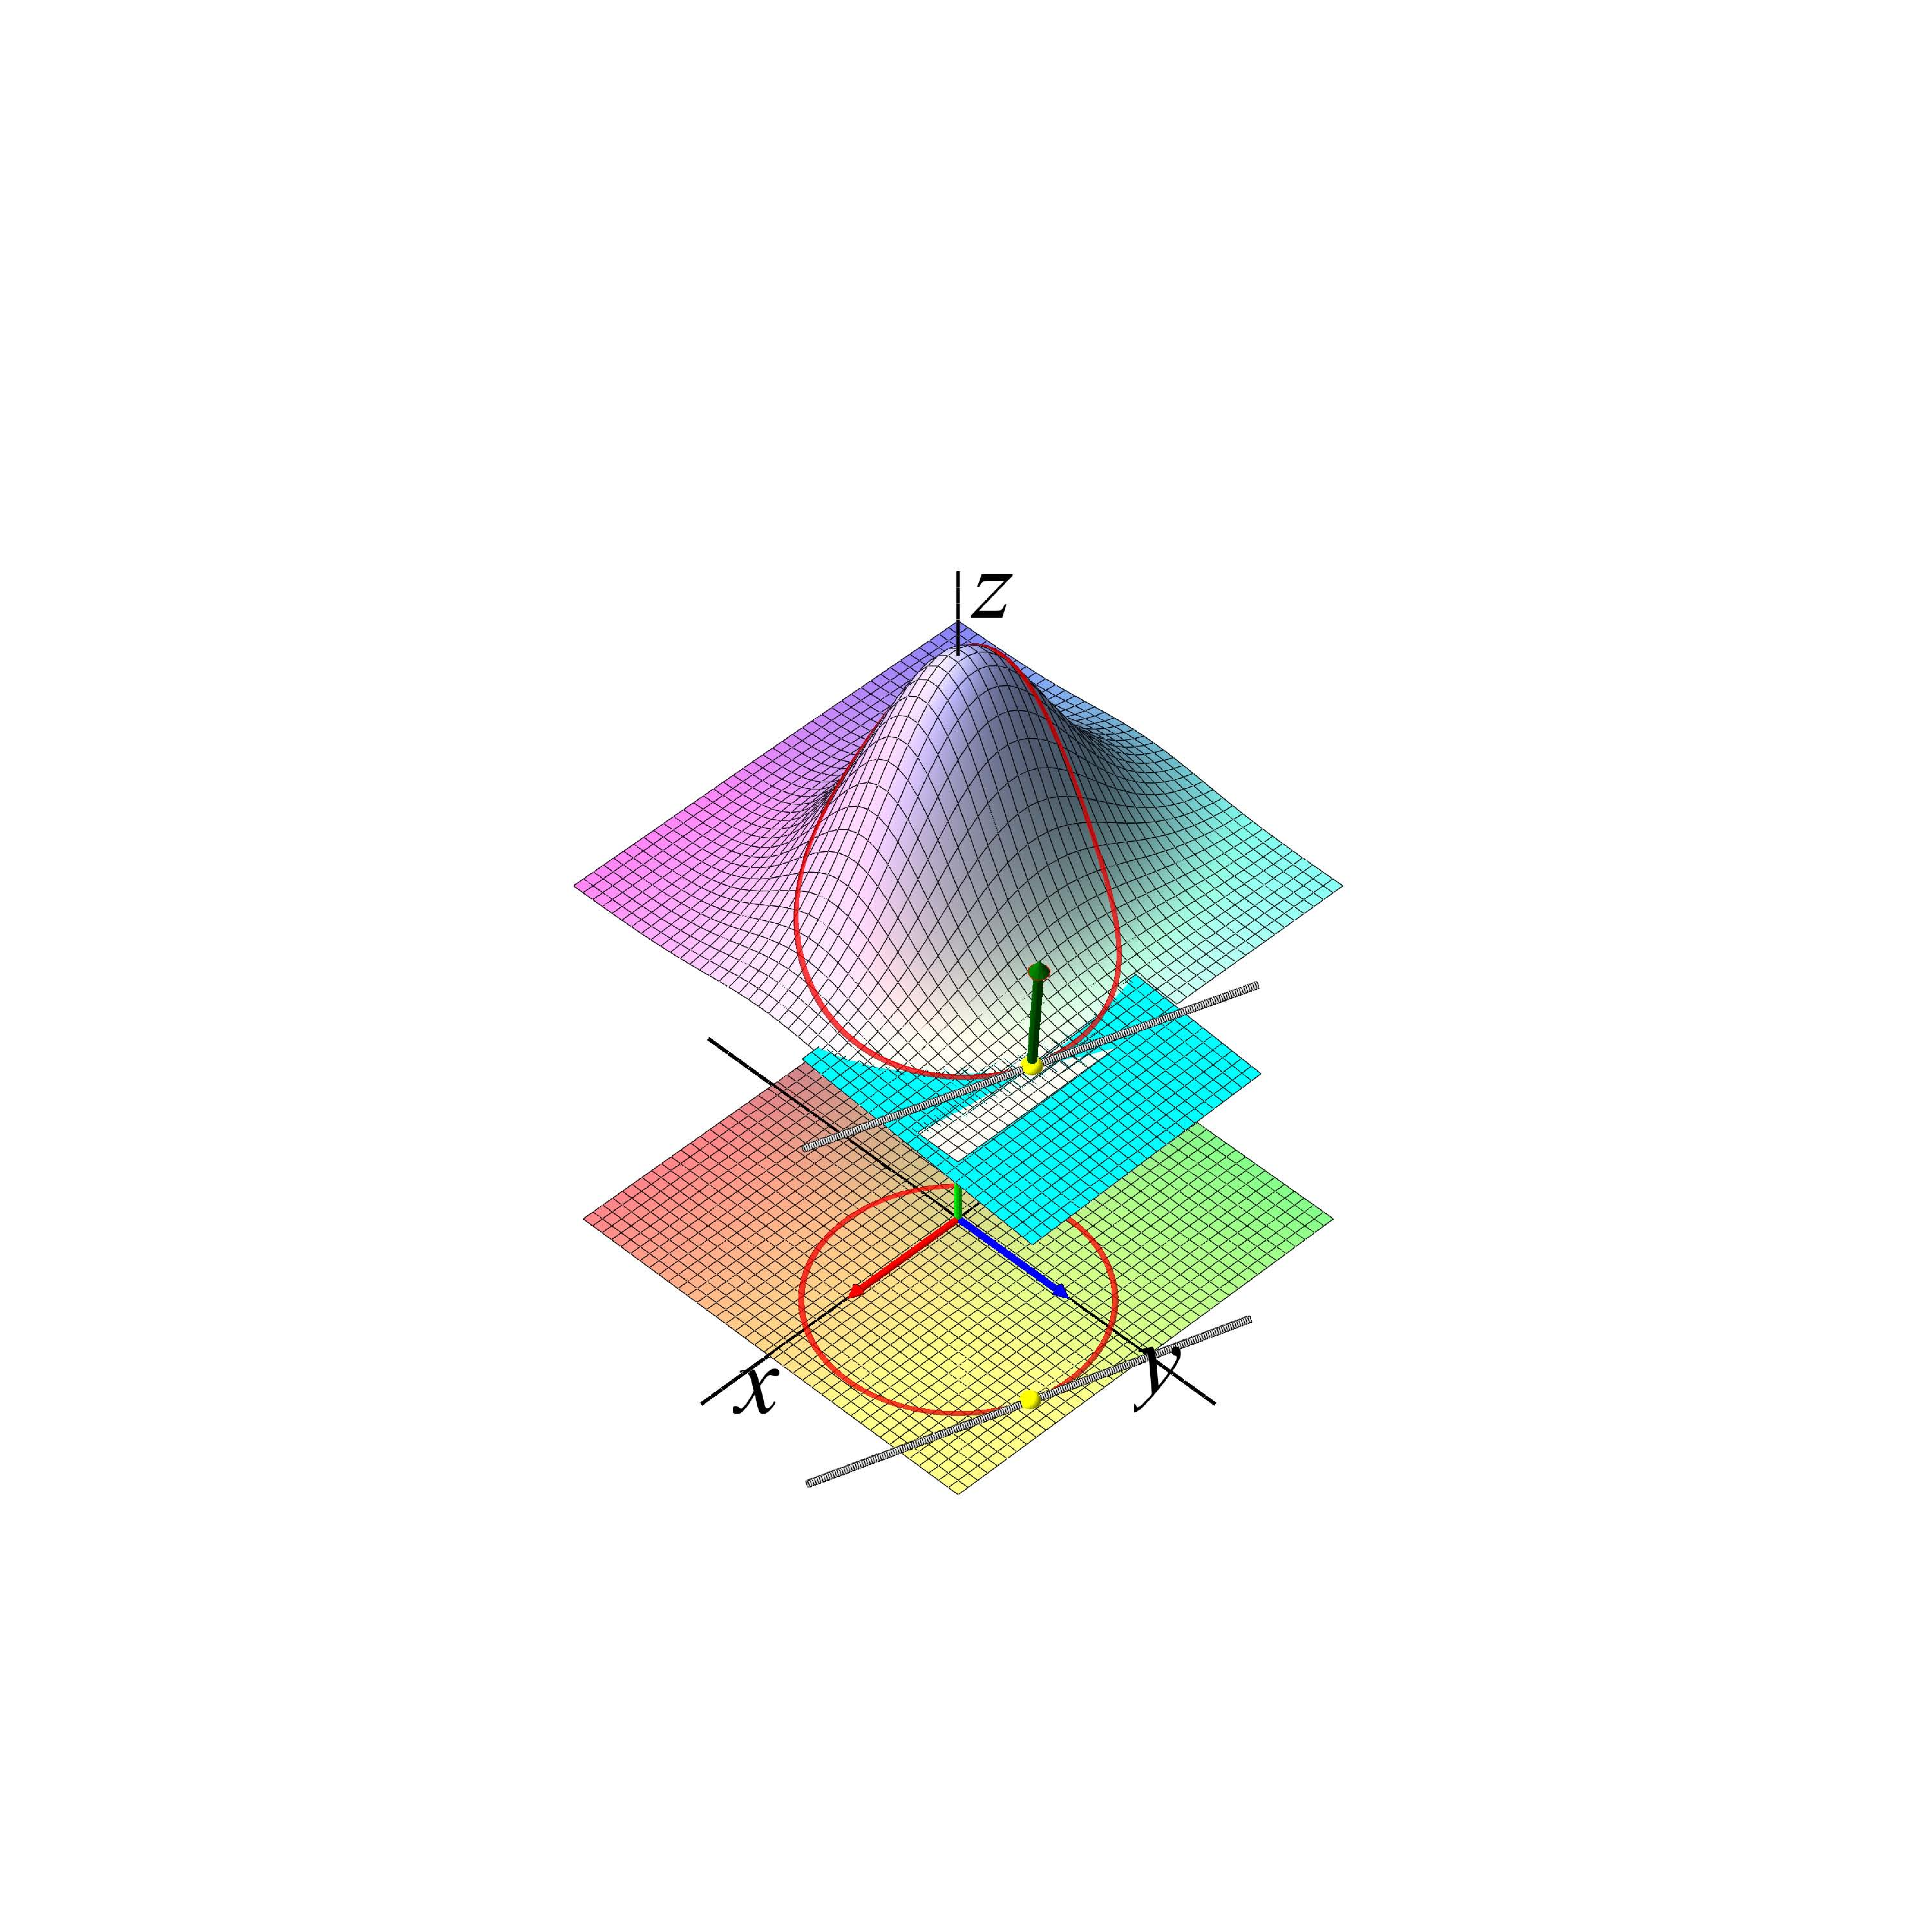
\includegraphics[height=105mm]{plotTangFull04B.pdf}}
\begin{center}
\caption{Grafen for $f(x,y) = 3 +  2\,\e^{-x^{2} - 2y^{2}}$  og tangentplanen igennem et tredje udvalgt punkt på den løftede cirkel, se figur \ref{figMainF}.} \label{figMainFTplanerC}
\end{center}
\end{figure}





\begin{theorem}[Tangenterne ligger i tangentplanen] \label{thmTangentTangent}
Lad $f(x,y)$ være en differentiabel funktion af to variable og lad $\widetilde{\mathbf{r}}(u)$ betegne en løftet kurve igennem punktet $\widetilde{\mathbf{r}}(u_{0}) = (x_{0}, y_{0}, f(x_{0}, y_{0}))$ på graf-fladen $\mathcal{G}(f)$. Så er tangenten til den løftede kurve indeholdt i tangentplanen til $\mathcal{G}(f)$ for $f(x,y)$. \\

Med andre ord: Ethvert punkt $(x,y,z)$ som ligger på tangenten $\widetilde{L}_{u_{0}}$ tilfredsstiller også tangentpla\-nens lig\-ning:
\begin{equation}
z = P_{1, (x_{0}, y_{0})}(x,y) = f(x_{0}, y_{0}) + f'_{x}(x_{0}, y_{0})\cdot (x - x_{0}) + f'_{y}(x_{0}, y_{0})\cdot (y - y_{0}) \quad.
\end{equation}
\end{theorem}

\begin{bevis}
Vi skal blot indse, at tangentvektoren $\widetilde{\mathbf{r}}\,'(u_{0})$ er vinkelret på en normalvektor til tangentplanen. En sådan normalvektor konstrueres i næste afsnit (se nedenfor):
\begin{equation}
\mathbf{N}_{(x_{0}, y_{0})}(f) = (- f'_{x}(x_{0}, y_{0}), -f'_{y}(x_{0}, y_{0}), 1 ) \quad ,
\end{equation}
og da
\begin{equation}
\begin{aligned}
\widetilde{\mathbf{r}}\,'(u_{0}) &=  \left(p'(u_{0}), q'(u_{0}), {\bm{\nabla}}f(p(u_{0}), q(u_{0}))\bm{\cdot} (p'(u_{0}), q'(u_{0})) \right) \\
&= \left(p'(u_{0}), q'(u_{0}), \left(f'_{x}(x_{0}, y_{0}), f'_{y}(x_{0}, y_{0})\right) \bm{\cdot} (p'(u_{0}), q'(u_{0}))\right)
\quad ,
\end{aligned}
\end{equation}
får vi ortogonaliteten ved at beregne skalarproduktet:
\begin{equation}
\begin{aligned}
\widetilde{\mathbf{r}}\,'(u_{0}) \, {\bm{\cdot}} \, \mathbf{N}_{(x_{0}, y_{0})}(f) & = - f'_{x}(x_{0}, y_{0})\cdot p'(u_{0})  -f'_{y}(x_{0}, y_{0})\cdot q'(u_{0}) \\ & \qquad + 1\cdot \left(f'_{x}(x_{0}, y_{0}), f'_{y}(x_{0}, y_{0})\right) \bm{\cdot} (p'(u_{0}), q'(u_{0})) \\
&= 0 \quad .
\end{aligned}
\end{equation}
\end{bevis}


\section{Gradienten bestemmer normalvektoren}


En plan i rummet med ligningen
\begin{equation}
a\cdot x + b\cdot y + c \cdot z + d = 0
\end{equation}
har en  normalvektor $\mathbf{N} = (a,b,c)$ som altså fås direkte fra koefficienterne  til $x$, $y$, og $z$ i ligningen. Vi kan nu skrive ligningen  for tangentplanen for graf-fladen for $f(x,y)$ i punktet $(x_{0}, y_{0}, f(x_{0}, y_{0})$ på netop den form således:
\begin{equation}\label{eqTangPlan}
\begin{aligned}
& z = P_{1, (x_{0}, y_{0})}(x,y) \quad , \\
& z = f(x_{0}, y_{0}) + f'_{x}(x_{0}, y_{0})\cdot (x-x_{0}) + f'_{y}(x_{0}, y_{0})\cdot (y-y_{0}) \quad , \\
& \textrm{som er ækvivalent med:} \\
& - f'_{x}(x_{0}, y_{0})\cdot (x - x_{0}) - f'_{y}(x_{0}, y_{0})\cdot (y - y_{0}) + z - f(x_{0}, y_{0}) = 0 \quad ,\\
& \textrm{og dermed:}\\
& - f'_{x}(x_{0}, y_{0})\cdot x - f'_{y}(x_{0}, y_{0})\cdot y + z + d = 0 \quad ,
\end{aligned}
\end{equation}
hvor $ d = x_{0}\cdot f'_{x}(x_{0}, y_{0}) + y_{0} \cdot f'_{y}(x_{0}, y_{0}) - f(x_{0}, y_{0})$.\\

Normalvektoren til tangentplanen aflæses direkte af den sidste ligning i (\ref{eqTangPlan}):
\begin{equation}
\mathbf{N}_{(x_{0}, y_{0})}(f) = (- f'_{x}(x_{0}, y_{0}), -f'_{y}(x_{0}, y_{0}), 1 ) \quad .
\end{equation}

\begin{aha}
En normalvektor til tangentplanen for graf-fladen for $f(x,y)$ kan  altså 'bygges' af de samme ingredienser som gradienten til $f(x,y)$ --  de partielle afledede. Læg dog mærke til minusserne og $1$-tallet. Og bemærk, at gradienten er en vektor i planen, normalvektoren er  en vektor i rummet.\\
\end{aha}

En alternativ udledning af normalvektorens koordinater fås på følgende måde: Hvis vi kan finde to lineært uafhængige vektorer i tangentplanen, så er deres krydsprodukt en normalvektor til planen.\\

Vi kender altid to \emph{lineært uafhængige vektorer i tangentplanen} igennem $(x_{0}, y_{0}, f(x_{0}, y_{0}))$, nemlig tangentvektorerne  til de løftede koordinatkurver igennem punktet, dvs.
\begin{equation}
\begin{aligned}
\widetilde{\mathbf{r}}\,'_{1}(x_{0}) &= (1, 0, f'_{x}(x_{0}, y_{0})) \quad , \\
\widetilde{\mathbf{r}}\,'_{2}(y_{0}) &= (0, 1, f'_{y}(x_{0}, y_{0})) \quad .
\end{aligned}
\end{equation}
En normalvektor til tangentplanen er derfor
\begin{equation}
\begin{aligned}
\mathbf{N}_{(x_{0}, y_{0})}(f) &= \widetilde{\mathbf{r}}\,'_{1}(x_{0})\, \times \,\widetilde{\mathbf{r}}\,'_{2}(y_{0}) \\
&= (- f'_{x}(x_{0}, y_{0})\, , \, \, -f'_{y}(x_{0}, y_{0}), 1 )
\end{aligned}
\end{equation}
- altså præcis den samme normalvektor som fundet ovenfor. \\


De to tangentvektorer $\widetilde{\mathbf{r}}\,'_{1}(x_{0})$ og  $\widetilde{\mathbf{r}}\,'_{2}(y_{0})$ giver os ligeledes en  \ind{parameterfremstilling for tangentplanen}{parameterfremstilling for tangentplanen}:

\begin{theorem}[Parameterfremstilling for tangentplaner]
Tangentplanen igennem punktet $(x_{0}, y_{0}, f(x_{0}, y_{0}))$ på graf-fladen $\mathcal{G}(f)$ for funktionen $f(x,y)$ har parameterfremstillingen
\begin{equation}
\begin{aligned}
\mathcal{T}_{(x_{0}, y_{0})}(f) \, \,&: \, \, \mathbf{T}(t_{1}, t_{2}) = (x_{0}, y_{0}, f(x_{0}, y_{0})) + t_{1}\cdot \widetilde{\mathbf{r}}'_{1}(x_{0}) + t_{2}\cdot \widetilde{\mathbf{r}}'_{2}(y_{0}) \\
&= (x_{0}, y_{0}, f(x_{0}, y_{0}))+ t_{1}\cdot(1, 0, f'_{x}(x_{0}, y_{0})) +   t_{2}\cdot (0, 1, f'_{y}(x_{0}, y_{0})) \, \, ,
\end{aligned}
\end{equation}
hvor $t_{1} \in \mathbb{R}$ og $t_{2} \in \mathbb{R}$.
\end{theorem}

\begin{example}[Løftede koordinatkurver]
Enhedsnormalvektoren i retningen $\mathbf{N}$  til de tangentplaner, der er vist i figurerne \ref{figMainFTplanerA}, \ref{figMainFTplanerB}, \ref{figMainFTplanerC} er også indtegnet på de figurer.
Desuden ses koordinatkurverne i $(x,y)$-planen samt de løftede koordinatkurver på graf-fladerne, dels for funktionen $f(x,y)$ og dels for de respektive
approksimerende førstegradspolynomier (tangentplanerne).
\end{example}

\begin{example}[Funktioner af \'{e}n variabel]
Enhver funktion af \'{e}n variabel kan betragtes som en funktion af to variable. Vi må forvente, at niveau-kurverne, gradientvektorfelterne, tangentplanerne, etc. er forholdsvis simple for sådanne funktioner. Vi ser på nogle eksempler, der viser det:
\begin{enumerate}
\item Funktionen $f(x,y) = x^{2}$ har følgende gradientfelt, tangentplaner, og normalvektorer:
\begin{equation}
\begin{aligned}
{\bm{\nabla}}f(x,y) &= (2x, 0) \quad ,\\
\mathcal{T}_{(x_{0}, y_{0})}(f) \quad : \quad \mathbf{T}(t_{1}, t_{2}) &= (x_{0} + t_{1}\, , \,\, y_{0} + t_{2}\, , \,\, x_{0}^{2} + 2x_{0}\cdot t_{1}) \quad ,\\
\mathbf{N}_{(x_{0}, y_{0})}(f) &= (-2x_{0}, 0, 1) \quad .\\
\end{aligned}
\end{equation}
 Se figur \ref{figXianden} hvor niveu-kurverne, gradientvektorfeltet, og graf-fladen er vist for funktionen.

 \item Funktionen $f(x,y) = x^{3}$ har
\begin{equation}
\begin{aligned}
{\bm{\nabla}}f(x,y) &= (3x^{2}, 0) \quad ,\\
\mathcal{T}_{(x_{0}, y_{0})}(f) \quad :  \quad \mathbf{T}(t_{1}, t_{2}) &= (x_{0} + t_{1}\, , \,\, y_{0} +  t_{2} \, , \,\, x_{0}^{3} + 3x_{0}^{2}\cdot t_{1}) \quad ,\\
\mathbf{N}_{(x_{0}, y_{0})}(f) &= (-3x_{0}^{2}, 0 , 1) \quad .\\
\end{aligned}
\end{equation}
 Se figur \ref{figXitredje} hvor kun niveu-kurverne og gradientvektorfeltet er vist. Sammenlign med niveaukurver og gradientvektorfeltet for $f(x,y) = x^{2}$ i figur \ref{figXianden}.


\item Funktionen $f(x,y) = \cos(3x)$ har
\begin{equation}
\begin{aligned}
{\bm{\nabla}}f(x,y) &= (- 3\sin(3x), 0) \quad ,\\
\mathcal{T}_{(x_{0}, y_{0})}(f) \quad : \quad \mathbf{T}(t_{1}, t_{2}) &= (x_{0} + t_{1}\, , \,\, y_{0} - t_{1}\cdot 3\sin(x_{0}) + t_{2}\, , \, \, \cos(3x_{0}))\quad ,\\
\mathbf{N}_{(x_{0}, y_{0})}(f) &= (3\sin(3x_{0}), 0, 1) \quad .\\
\end{aligned}
\end{equation}
 Se figur \ref{figCos3x}. Sammenlign med figur \ref{figCosPlusSin}. Inspektion af grafen og af niveaukurverne for funktionen i \ref{figCosPlusSin} leder til den ide, at man måske ved at dreje koordinatsystemet -- og dermed skifte koordinater i planen -- også  kan beskrive den funktion som en funktion af \'{e}n variabel. Det er da også tilfældet, idet
den viste funktion er $f(x,y) = \cos(3x + 3y)$.
\end{enumerate}
\end{example}

\begin{figure}[ht]
\centerline{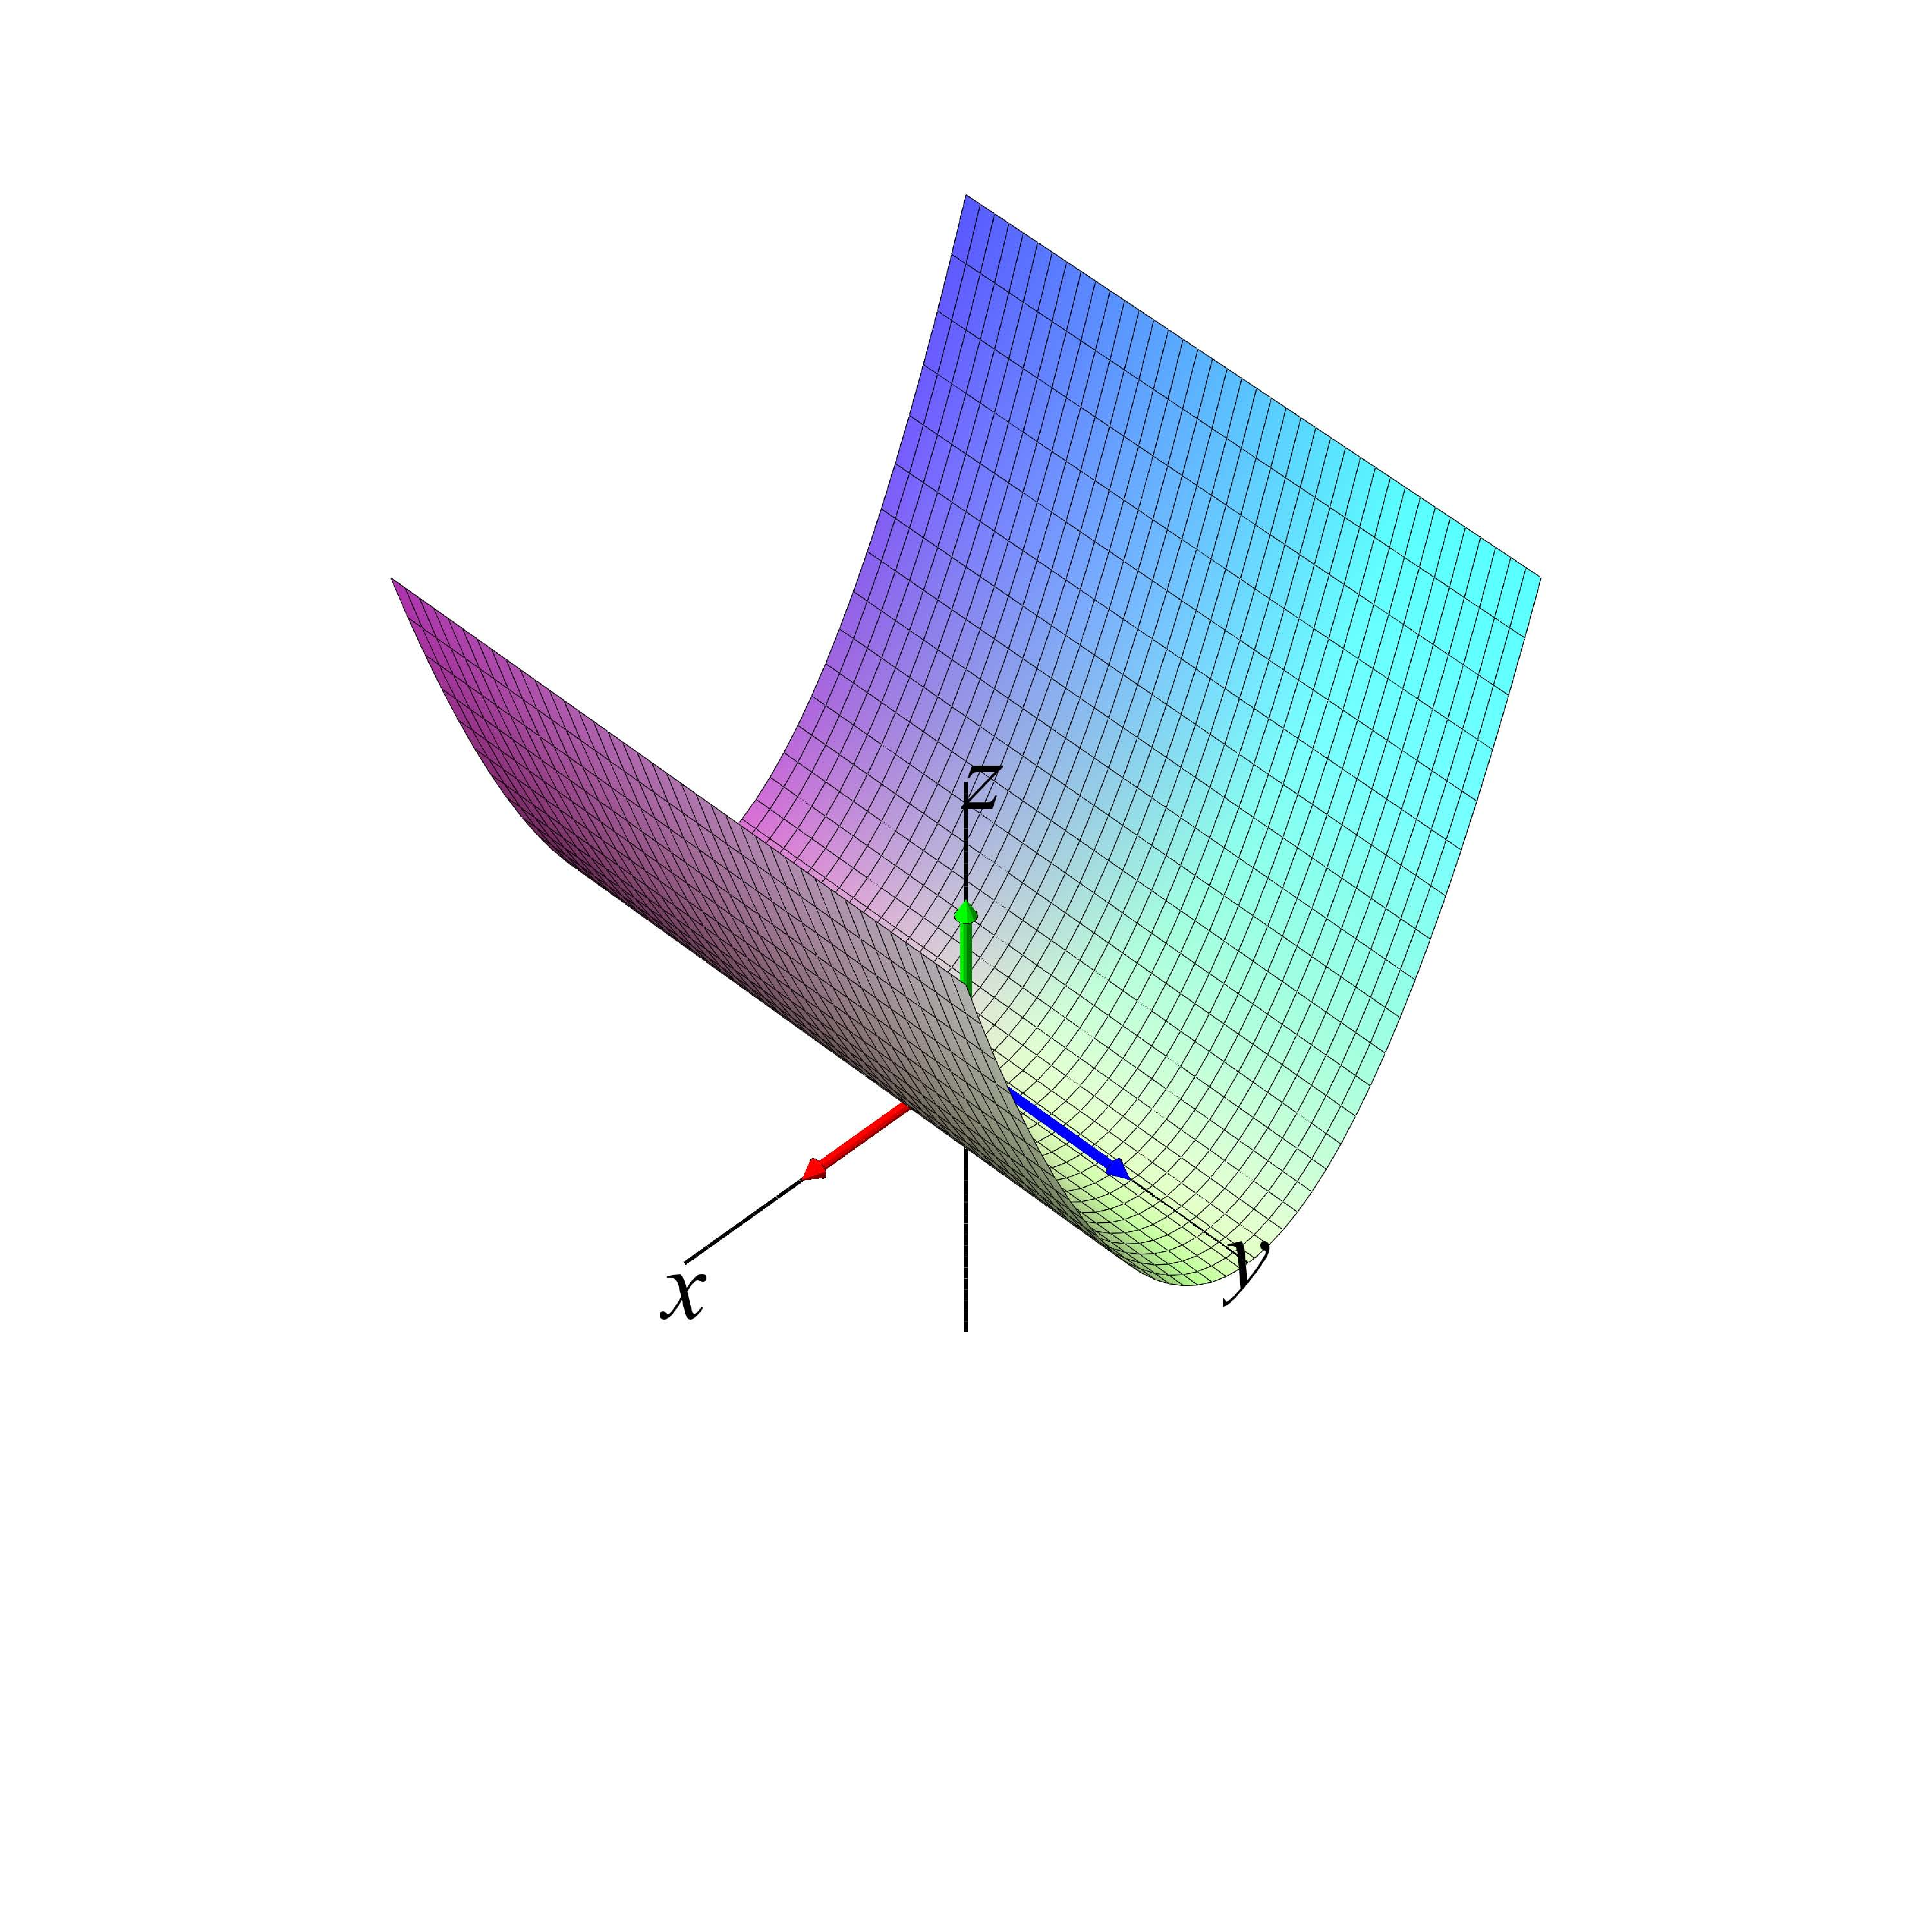
\includegraphics[height=80mm]{plotXianden.pdf} \quad 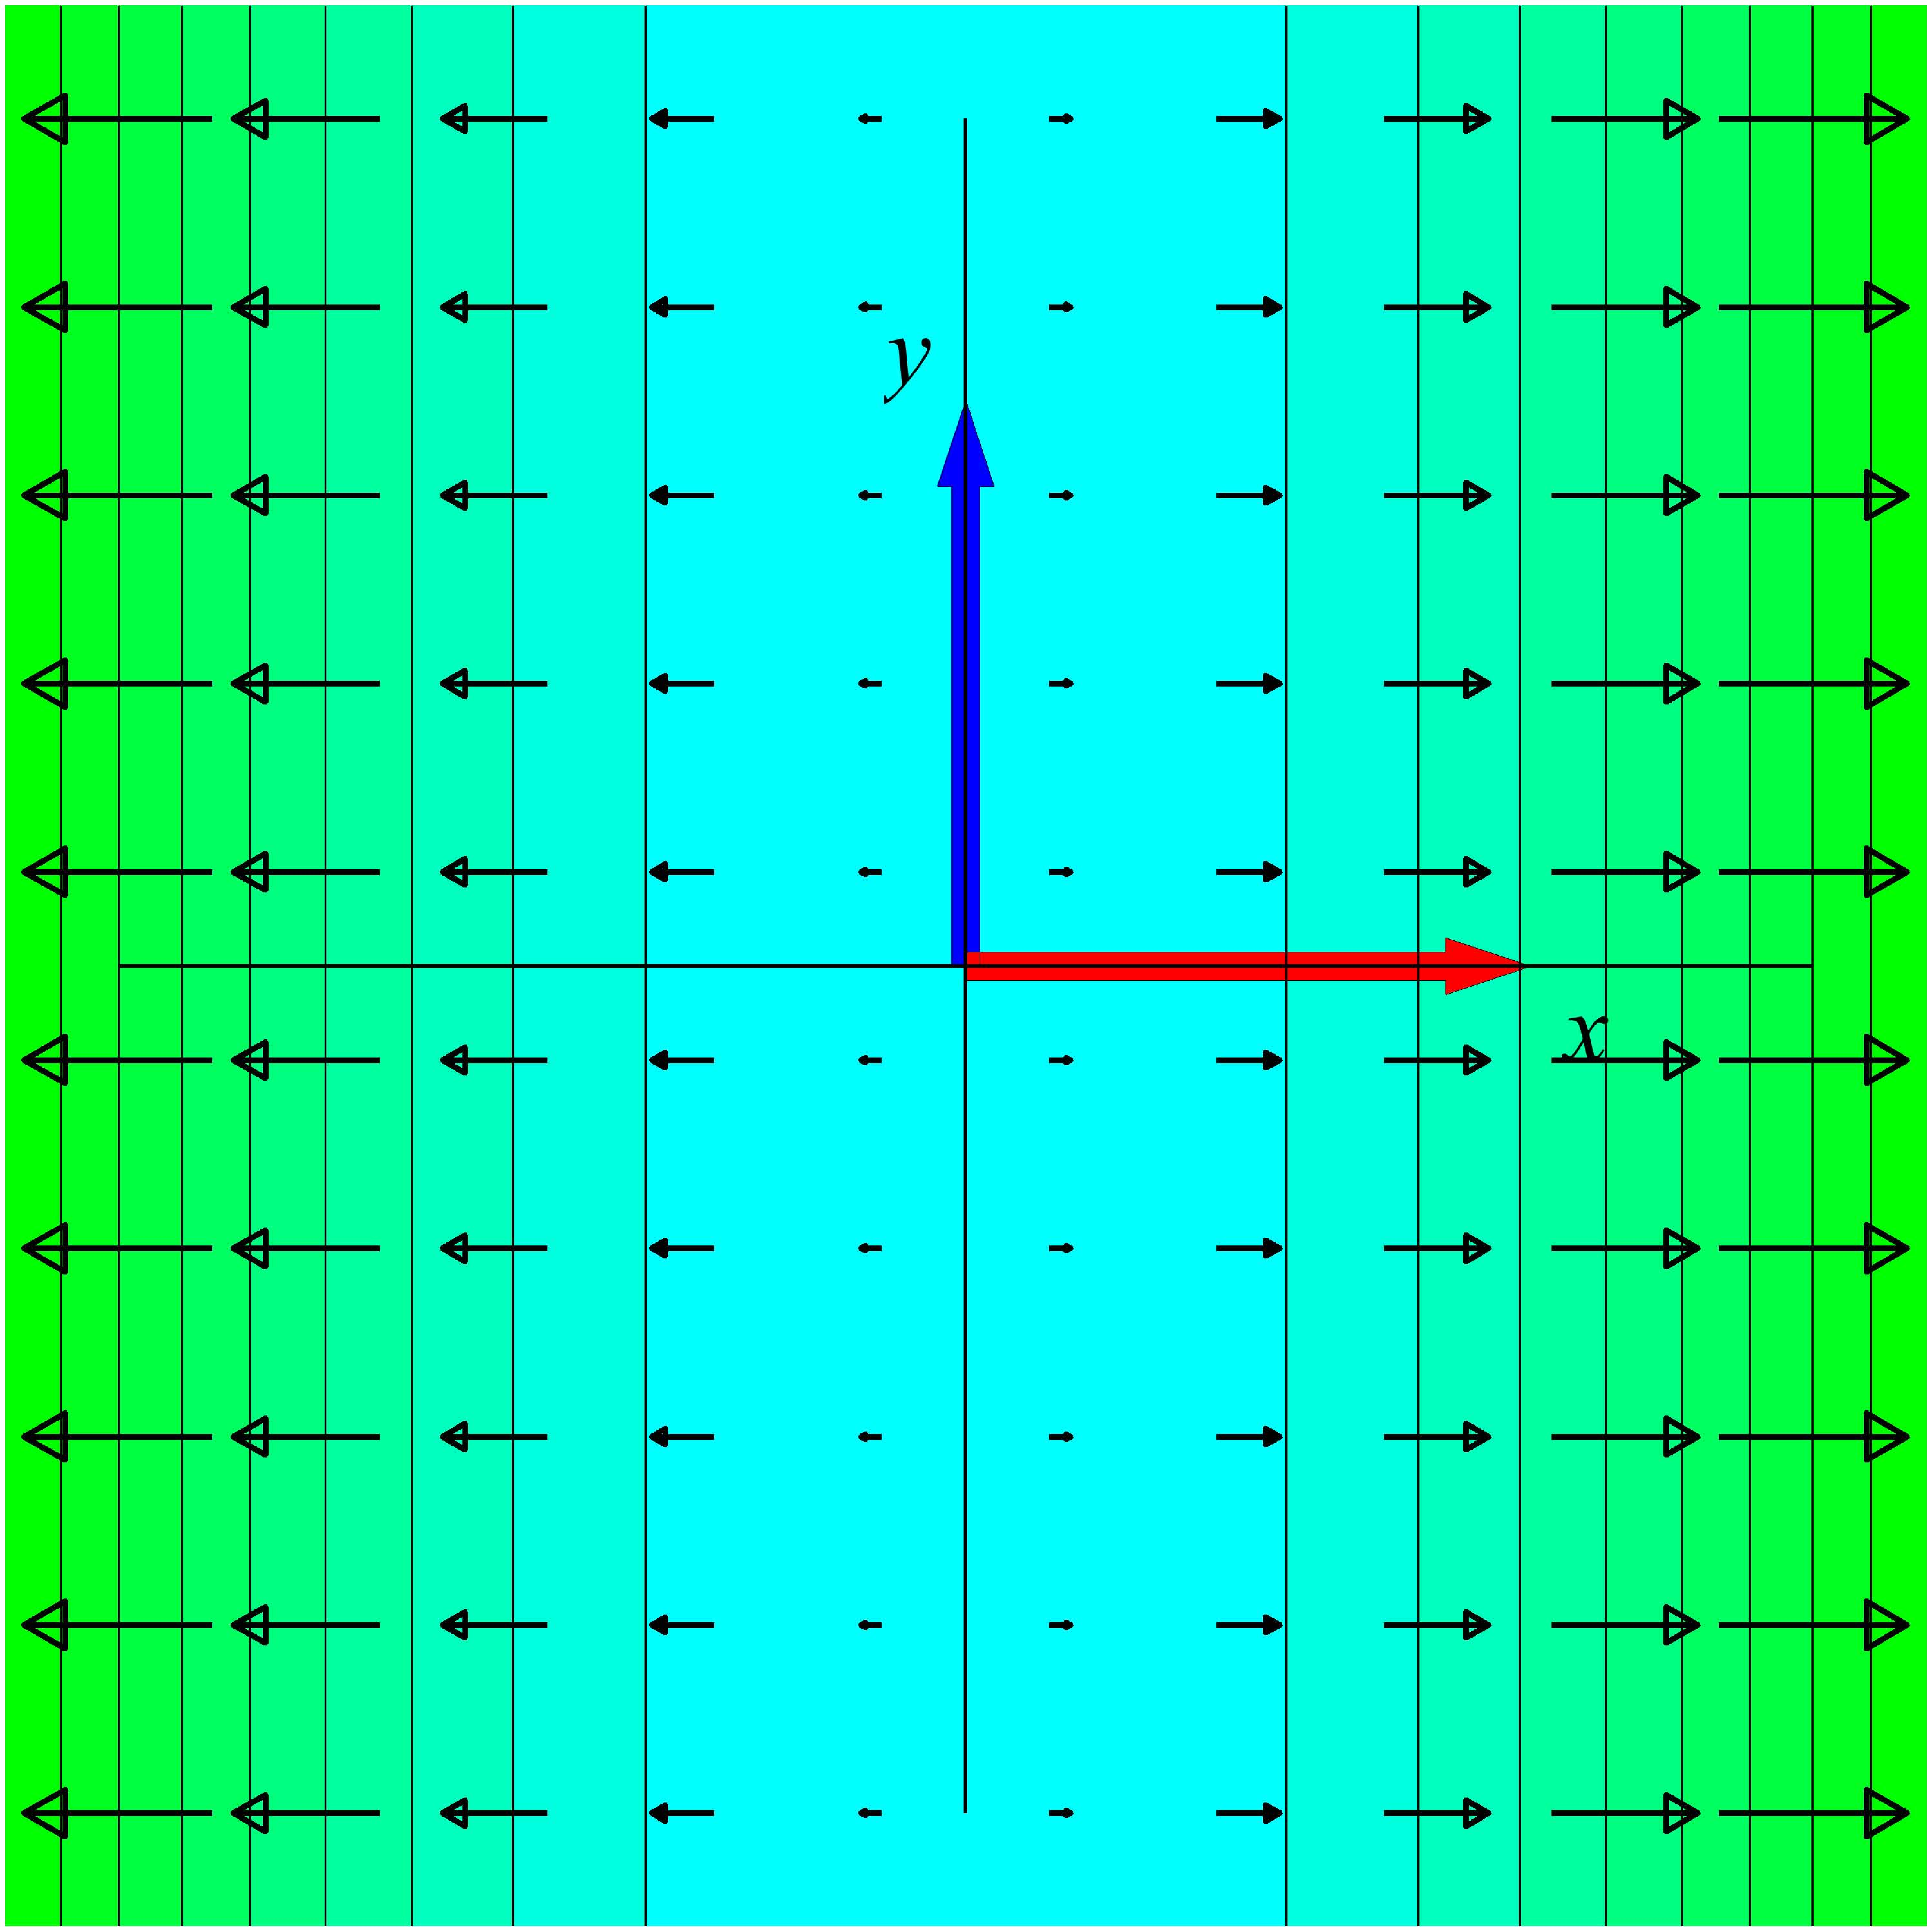
\includegraphics[height=35mm]{plotGradXianden.pdf}}
\begin{center}
\caption{Grafen  for $f(x,y) = x^{2}$ samt tilhørende niveaukurver og gradientvektorfelt i $(x,y)$-planen.} \label{figXianden}
\end{center}
\end{figure}

\begin{figure}[ht]
\centerline{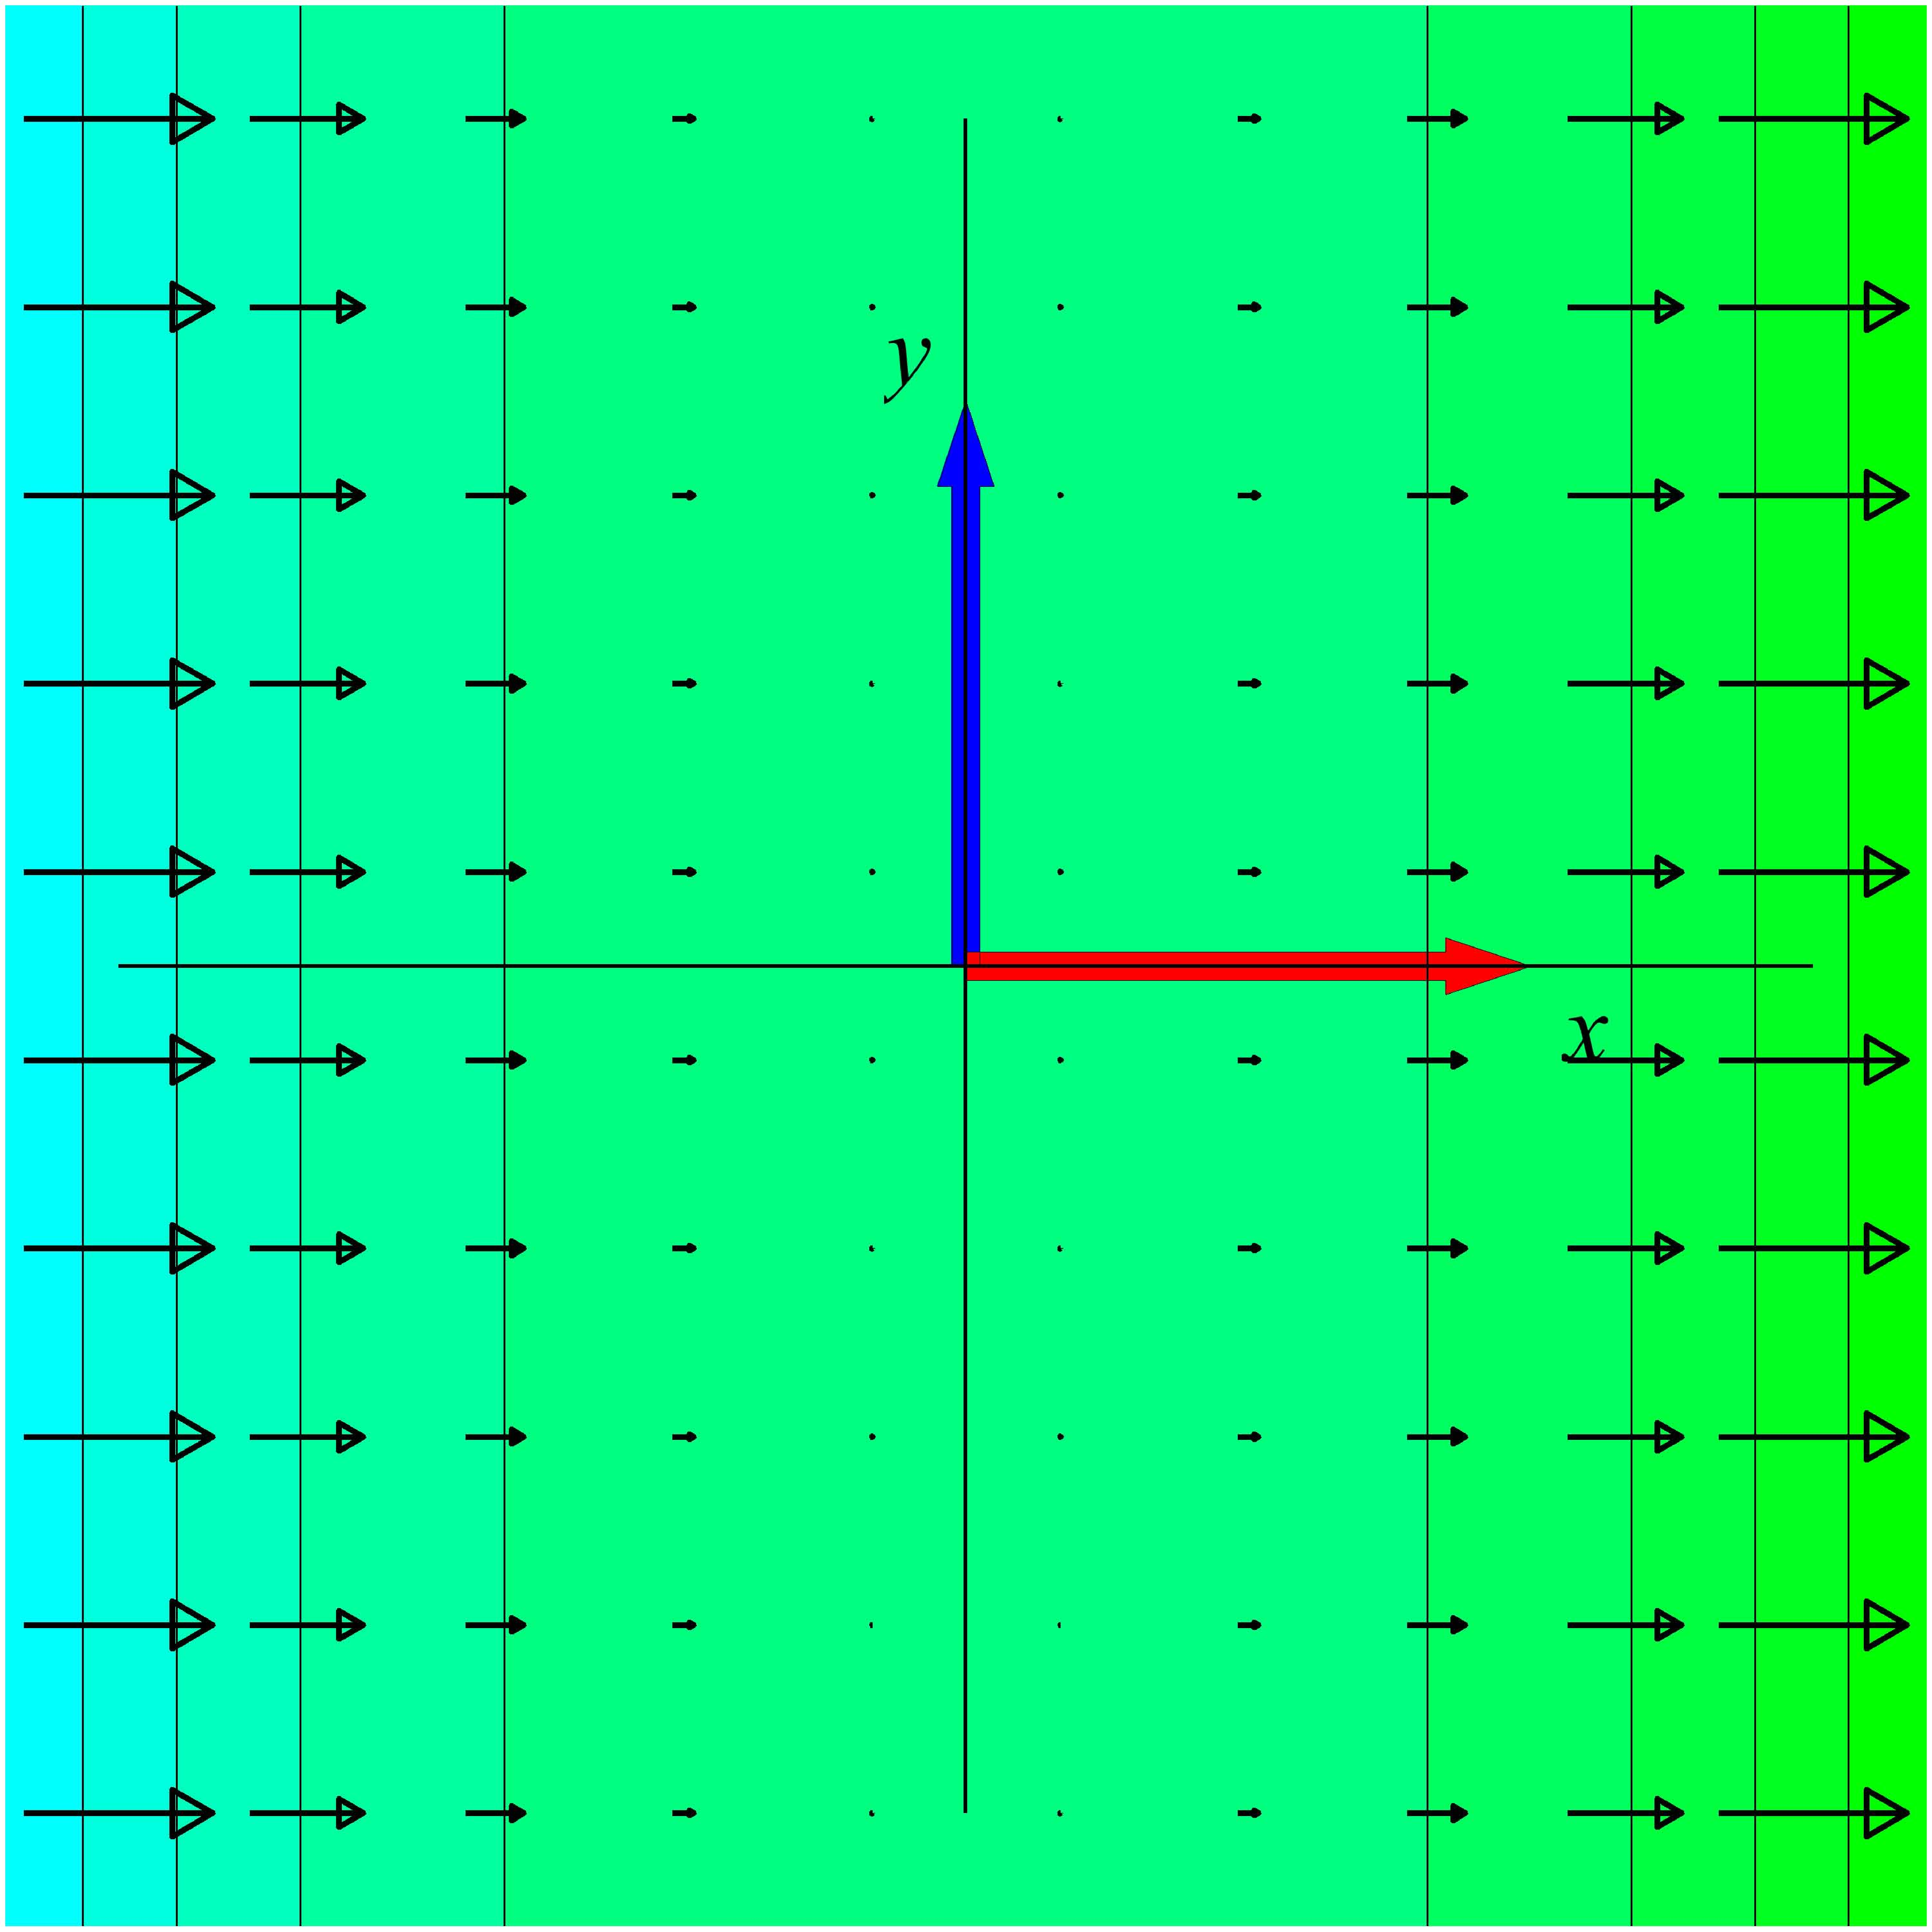
\includegraphics[height=35mm]{plotGradXitredje.pdf}}
\begin{center}
\caption{Niveaukurver og gradientvektorfelt for $f(x,y) = x^{3}$.} \label{figXitredje}
\end{center}
\end{figure}



\begin{figure}[ht]
\centerline{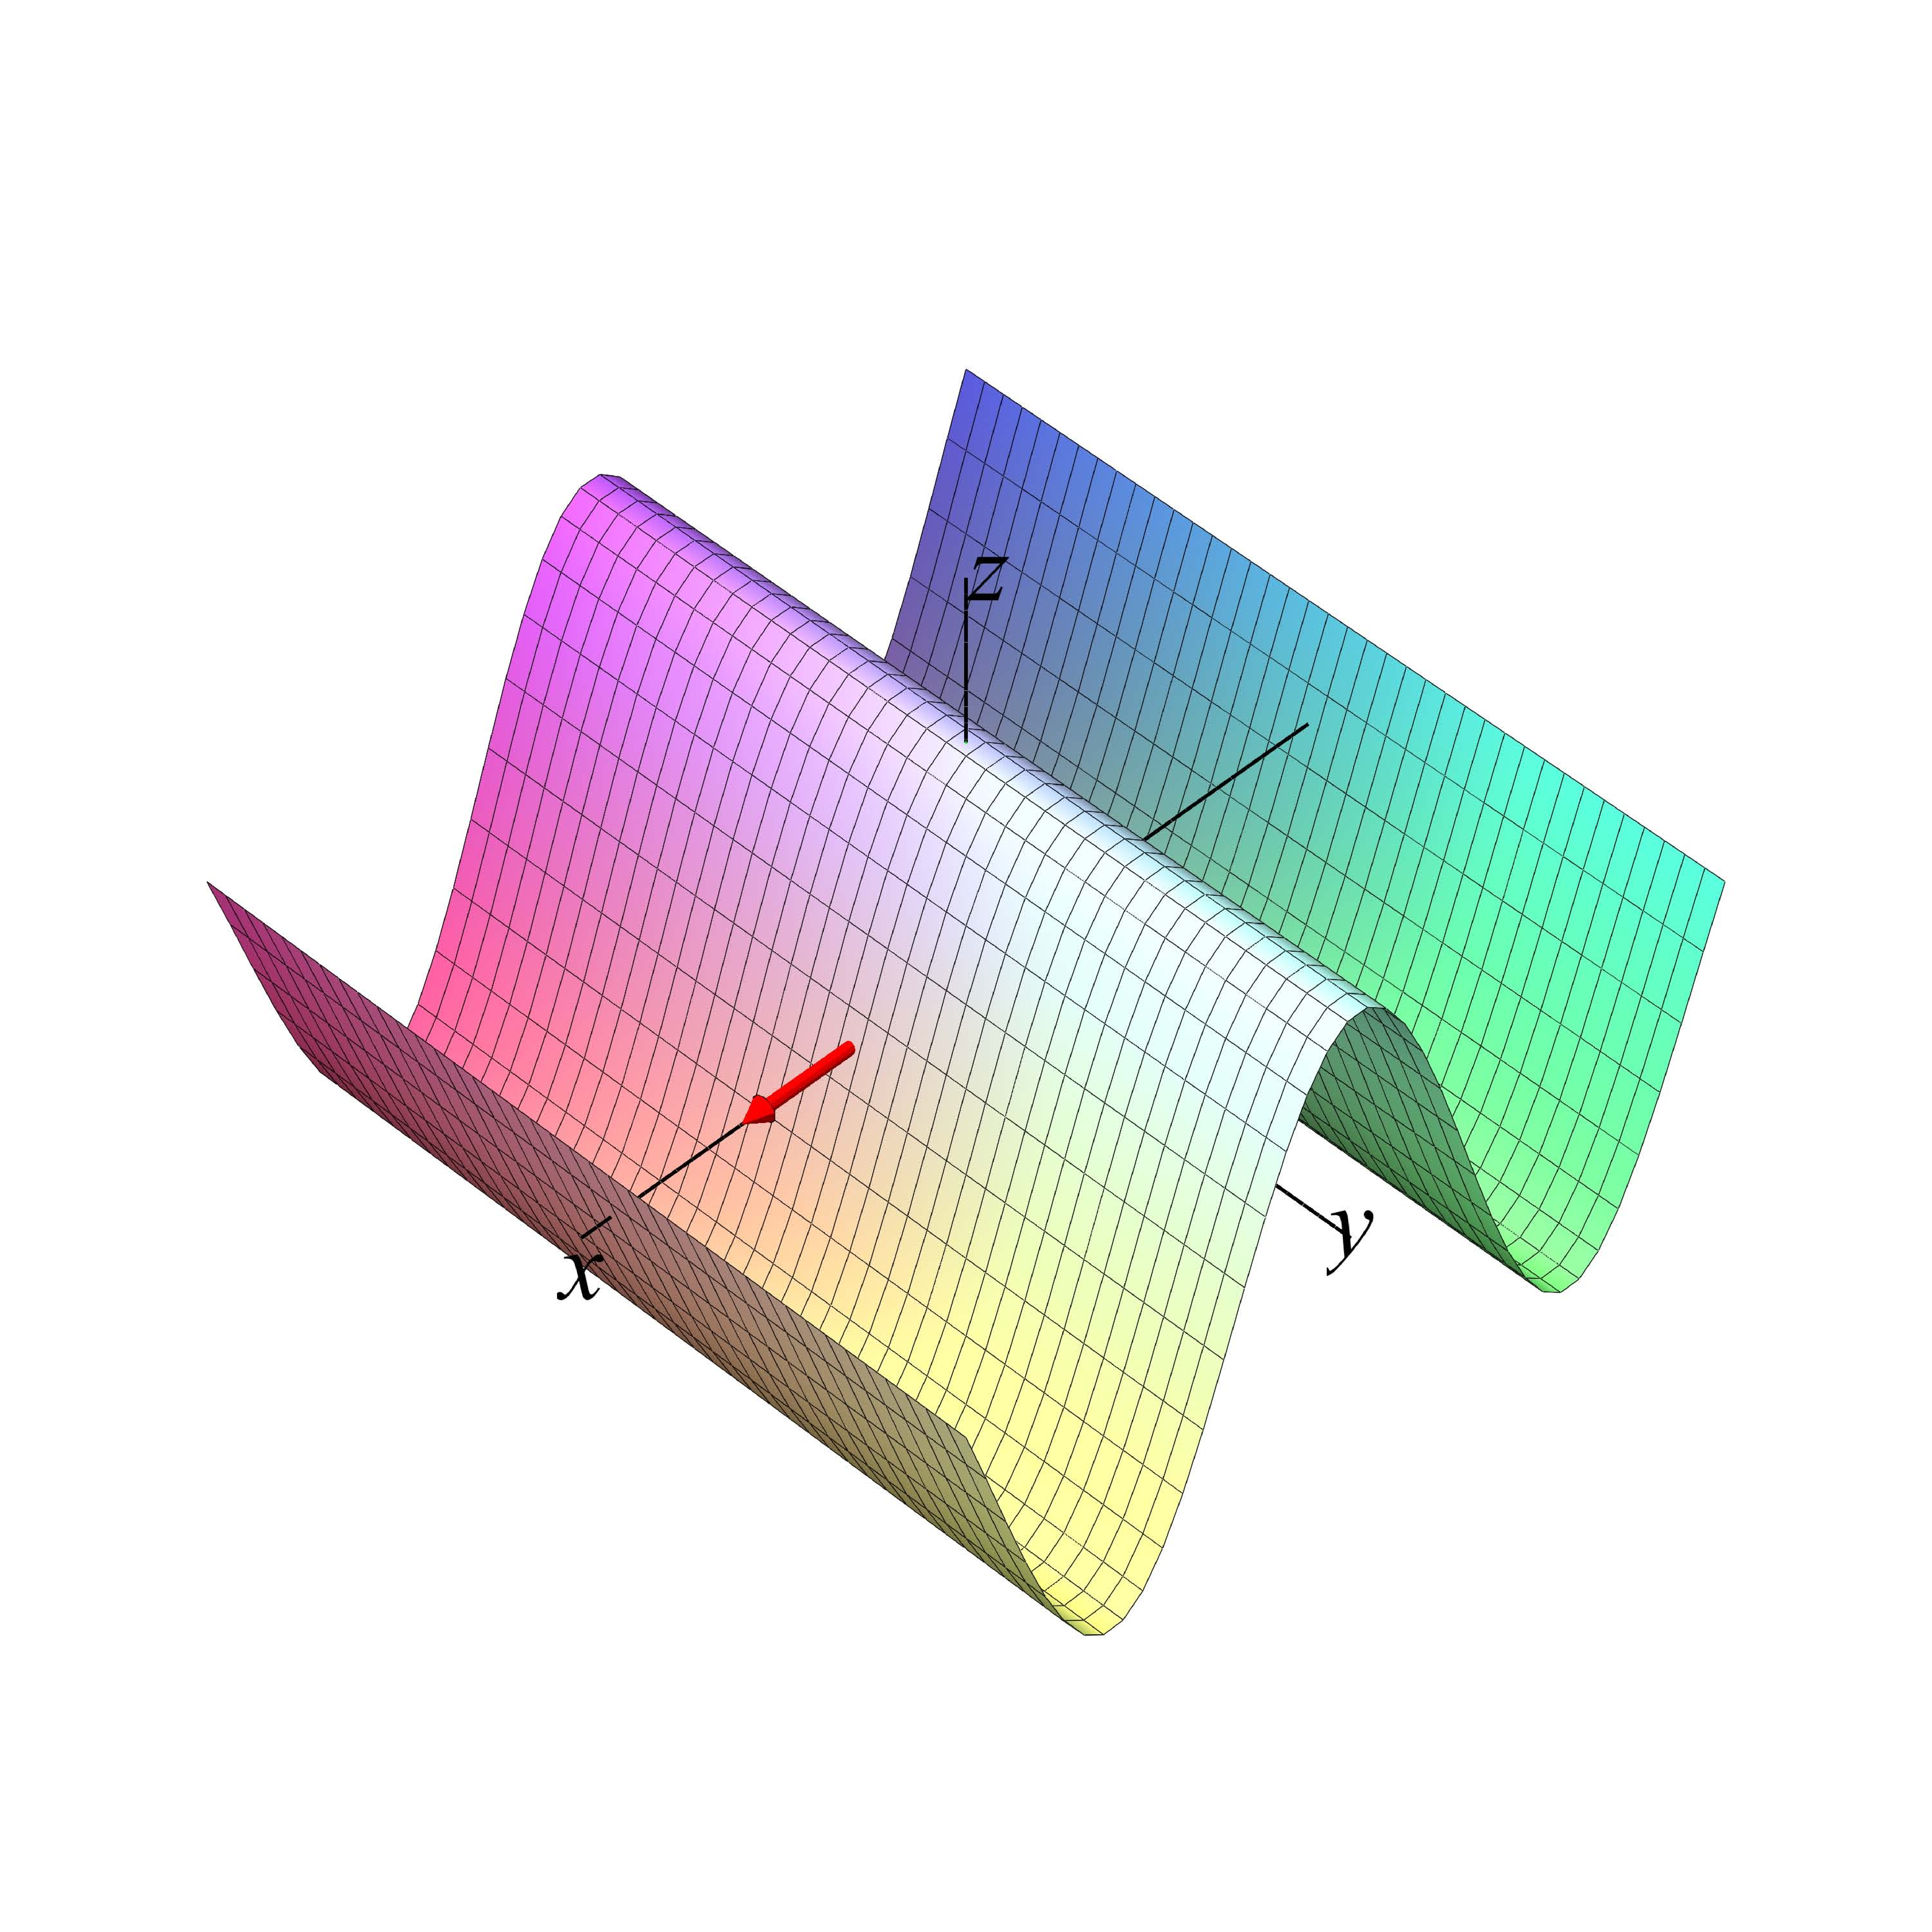
\includegraphics[height=80mm]{plotSurfCos3x.pdf} \quad 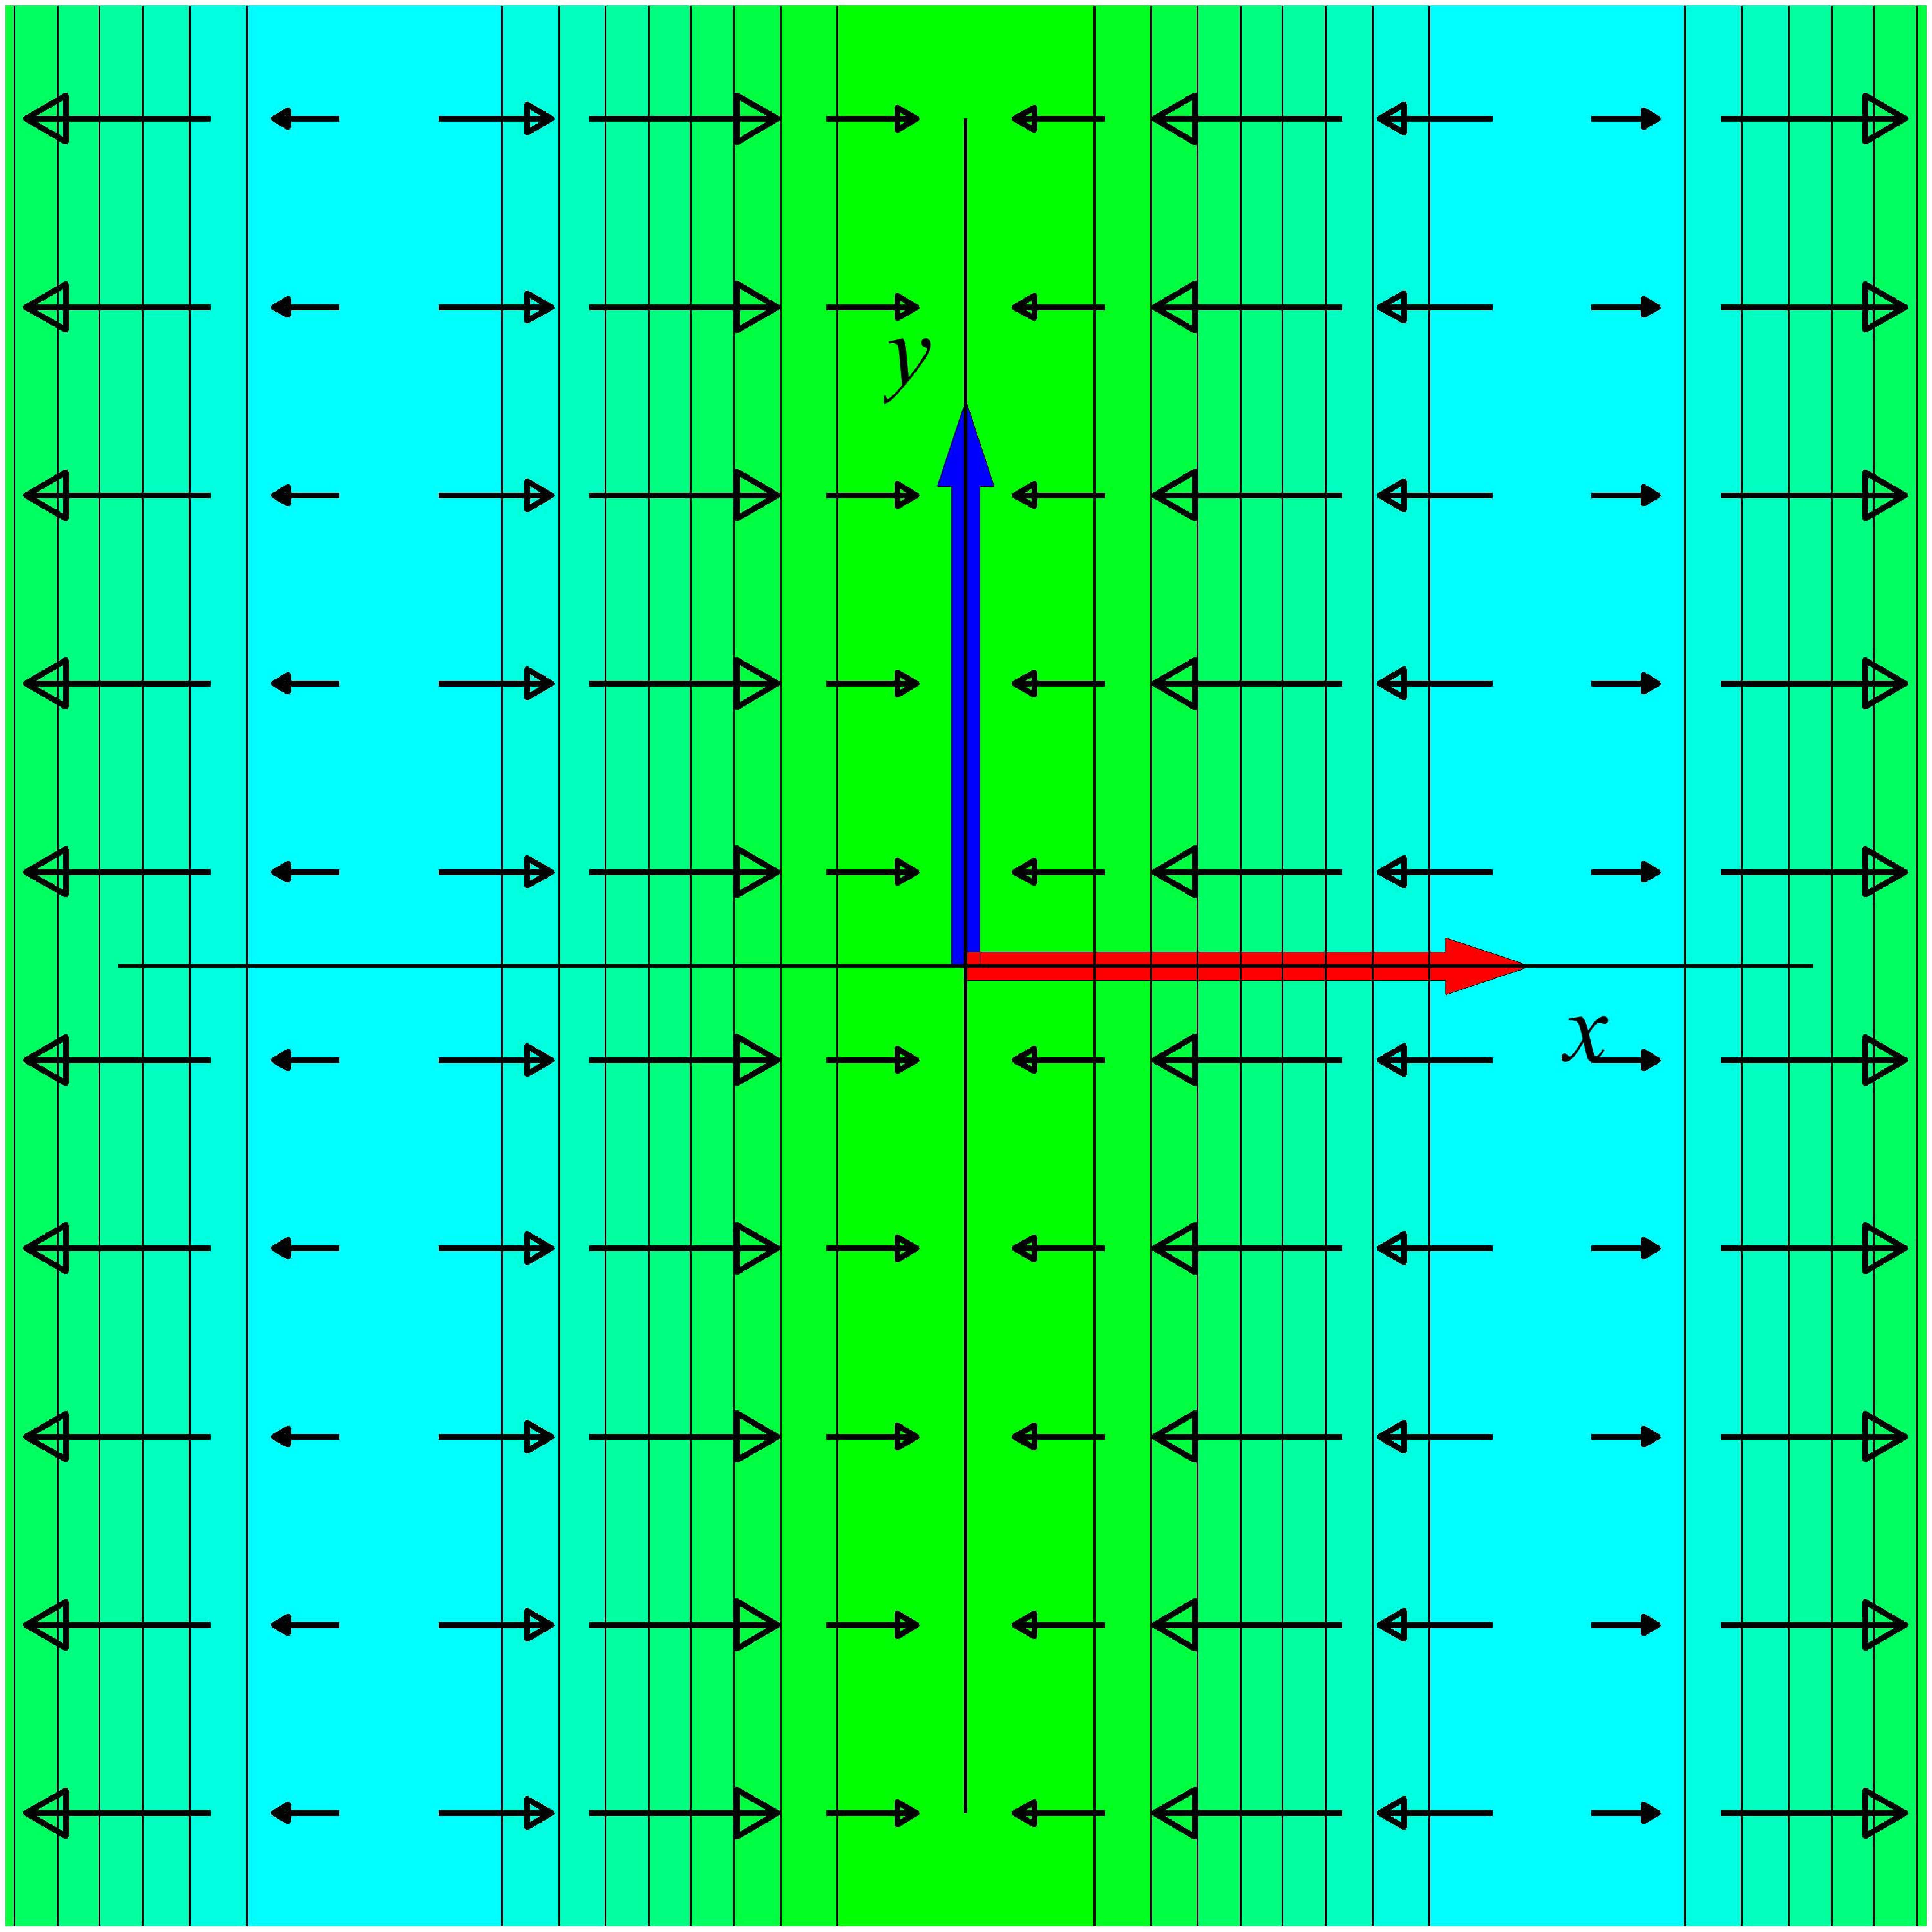
\includegraphics[height=35mm]{plotGradcos3x.pdf}}
\begin{center}
\caption{Grafen, niveaukurver, og gradientvektorfelt for $f(x,y) = \cos(3x)$.} \label{figCos3x}
\end{center}
\end{figure}

\begin{figure}[ht]
\centerline{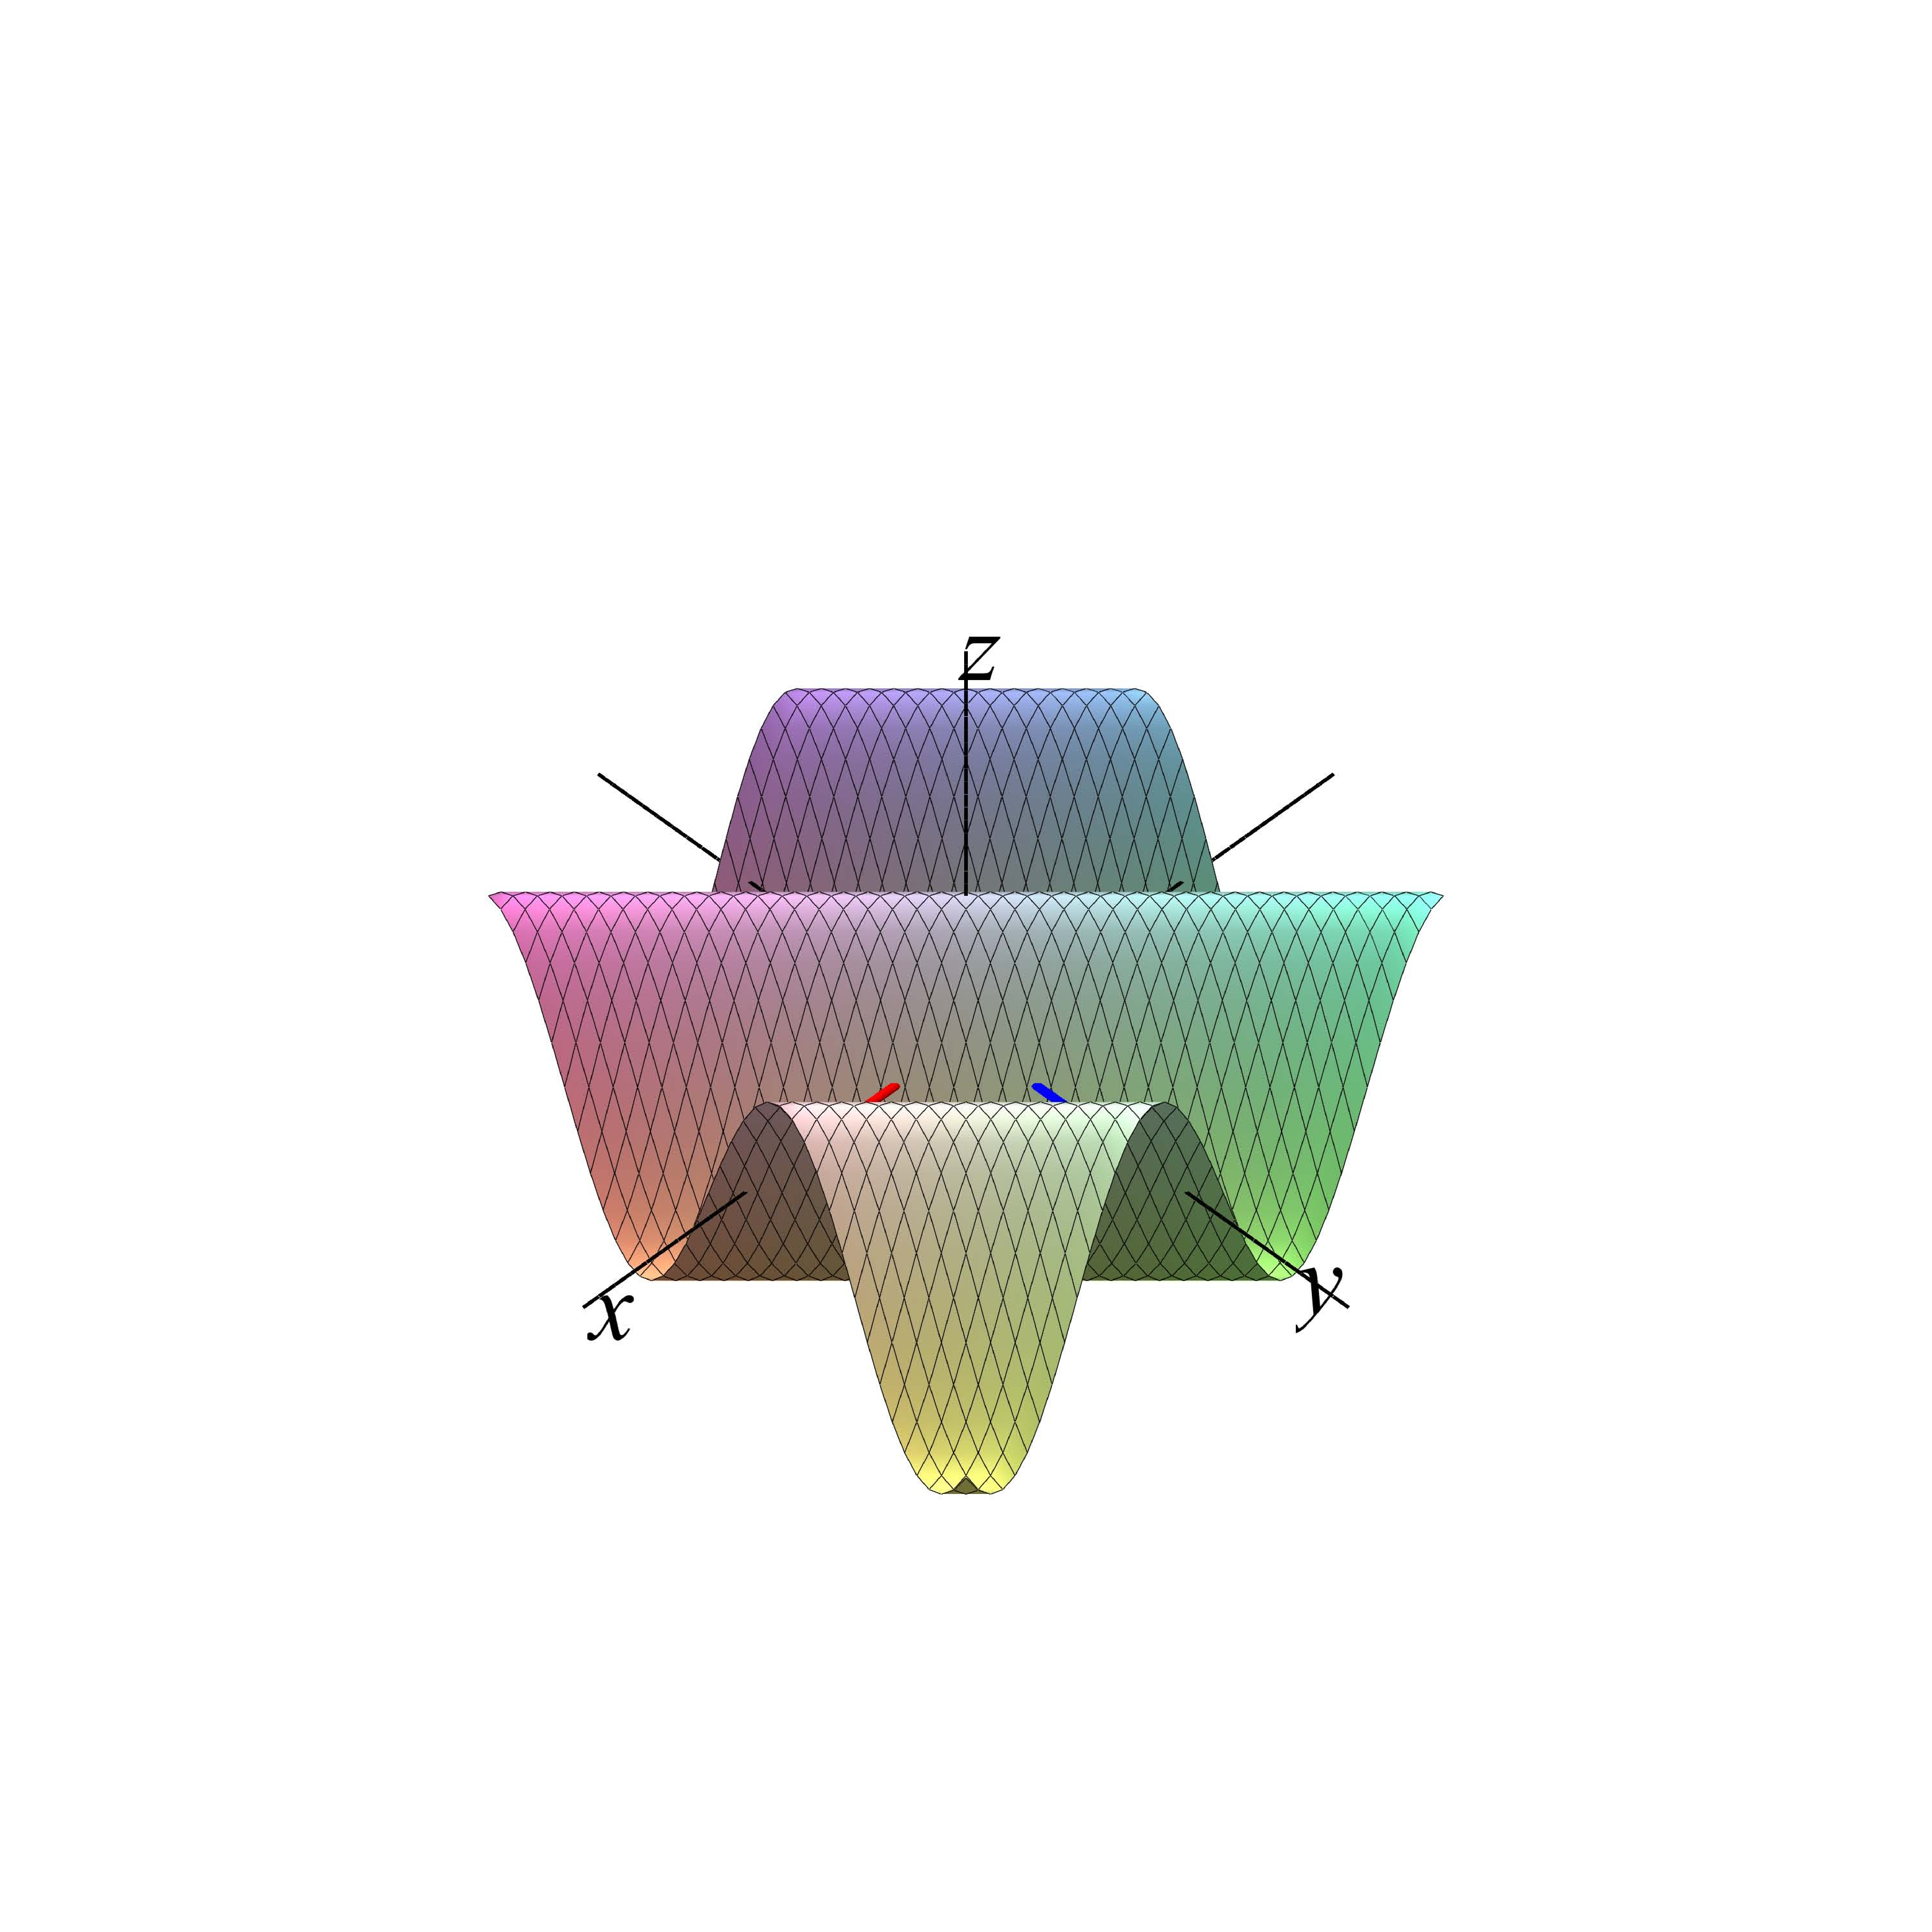
\includegraphics[height=80mm]{plotSurfCosXplusY.pdf} \quad 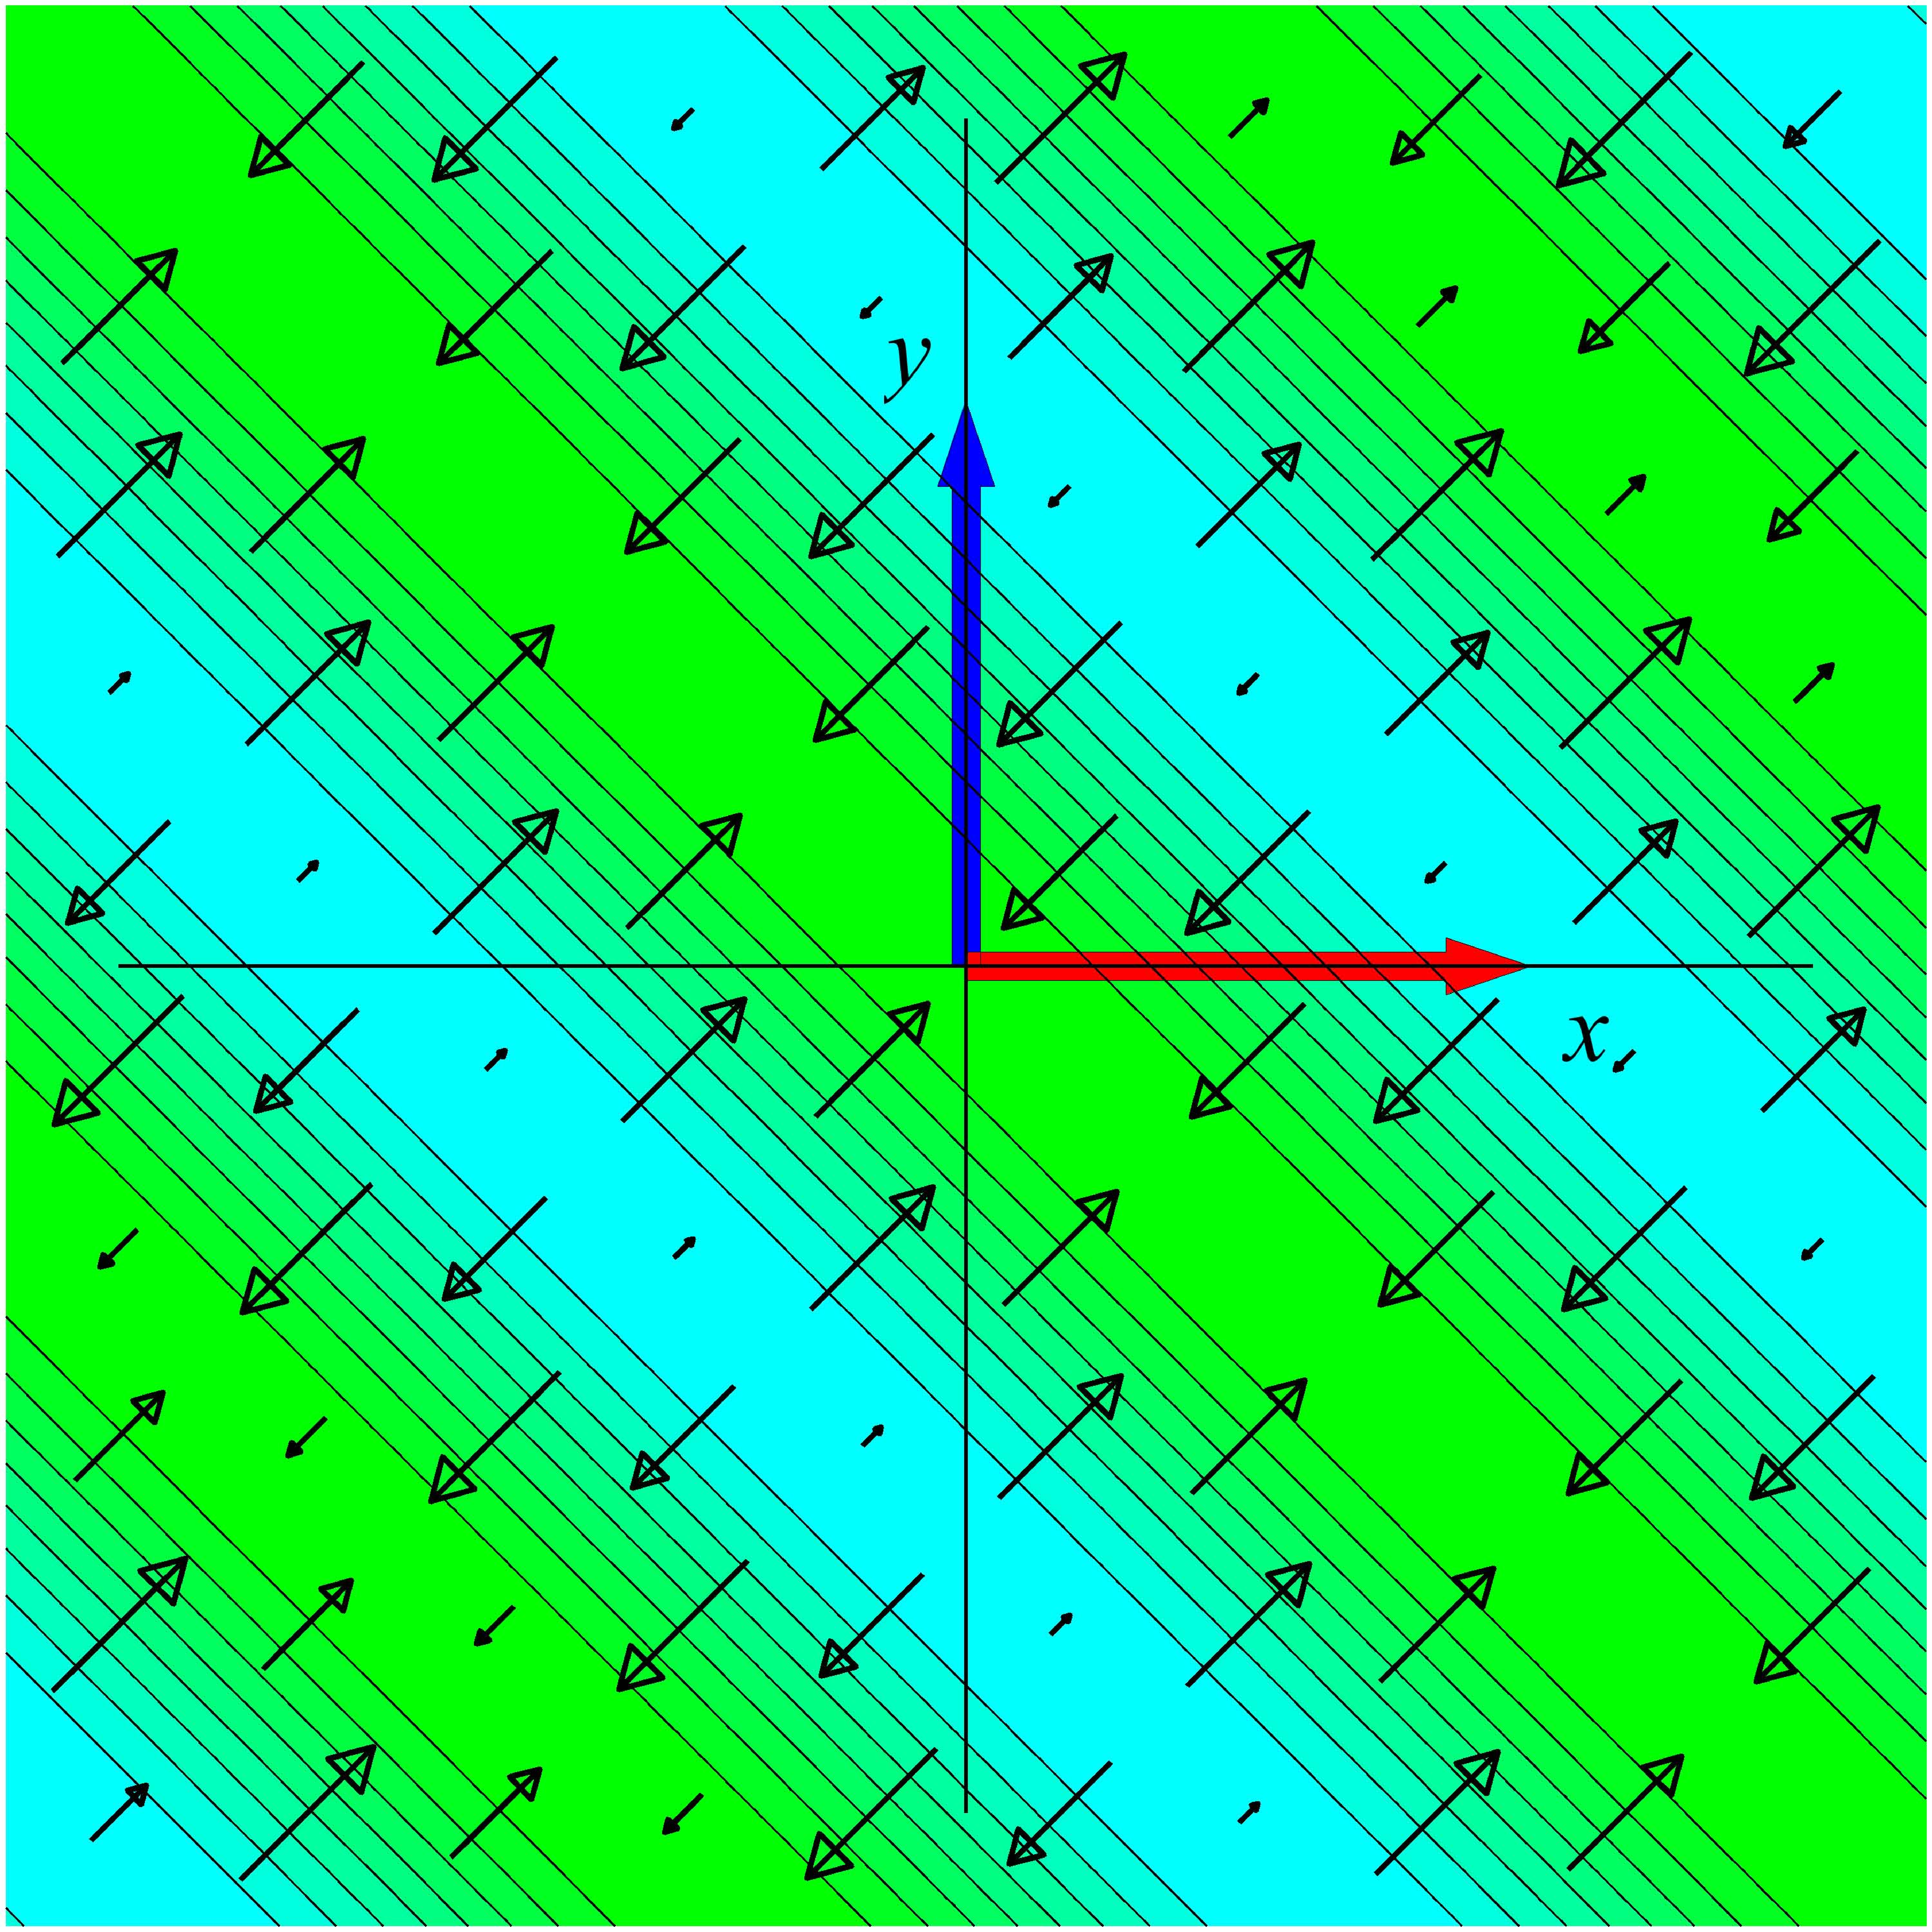
\includegraphics[height=35mm]{plotGradCosXplusY.pdf}}
\begin{center}
\caption{Grafen, niveaukurver, og gradientvektorfelt for $f(x,y) = \cos(3x+3y)$.} \label{figCosPlusSin}
\end{center}
\end{figure}



\begin{exercise}
Bestem enheds-normalvektoren til tangentplanerne igennnem punktet $(x_{0}, y_{0}, f(x_{0}, y_{0})$ på graf-fladerne for enhver af følgende funktioner for ethvert punkt $(x_{0}, y_{0})$ i $(x,y)$-planen.
\begin{equation}
\begin{aligned}
  f(x,y) &= 3x + y\\
  f(x,y) &= x^{2} + y^{2} \\
  f(x,y) &= y\cdot\e^{x} \quad.
\end{aligned}
\end{equation}
\end{exercise}

%%%%%%%%%%%%%%%%%%%%%%%%%%%%%%%%%%%%%%%%%%%%%%%%%%%
%%%%%%%%%%%%%%%%%%%%%%%%%%%%%%%%%%%%%%%%%%%%%%%%%%%
%%%%%%%%%%%%%%%%%%%%%%%%%%%%%%%%%%%%%%%%%%%%%%%%%%%

\begin{summary}
De partielle afledede af en funktion af to variable har forskellige
geometriske iklædninger, som er særdeles nyttige at bruge ved beskrivelse
og analyse af funktionerne. Gradientvektorfeltet -- der jo har de partielle afledede som koordinatfunktioner -- indeholder
(næsten) al information om funktionen. I denne eNote har vi arbejdet med følgende:
\begin{itemize}
\item Gradienten udpeger i ethvert punkt den retning hvori funktionen lokalt vokser mest og den (modsatte) retning hvori funktionen aftager mest.
\item Længden af gradienten for $f(x,y)$ i punktet $(x_{0}, y_{0}))$ er værdien af den største retningsafledede af $f(x,y)$ i punktet, og den tilsvarende negative værdi er værdien af den mindste retningsafledede i punktet.
\item Gradientvektorfeltet for $f(x,y)$ er overalt ortogonal på niveaukurverne for $f(x,y)$.
\item De løftede kurver på graf-fladen for en funktion har tangenter, der er helt indeholdt i tangentplanen til graf-fladen.
\item Tangentplanen til graf-fladen for funktionen $f(x, y)$ i et givet punkt $(x_{0}, y_{0}, f(x_{0}, y_{0}))$ har en normalvektor, der er 'bygget' op af de partielle afledede:
    \begin{equation*}
    \mathbf{N}_{(x_{0}, y_{0})}(f) = (- f'_{x}(x_{0}, y_{0})\, , \, \, -f'_{y}(x_{0}, y_{0}), 1 ) \quad .
    \end{equation*}
\item Tangentplanen til graf-fladen for funktionen $f(x, y)$ i et givet punkt $(x_{0}, y_{0}, f(x_{0}, y_{0}))$ er repræsenteret dels ved ligningen
\begin{equation*}
z = P_{1, (x_{0}, y_{0})}(x,y) = f(x_{0}, y_{0}) + f'_{x}(x_{0}, y_{0})\cdot (x - x_{0}) + f'_{y}(x_{0}, y_{0})\cdot (y - y_{0})
\end{equation*}
og dels ved parameterfremstillingen
\begin{equation*}
\begin{aligned}
\mathcal{T}_{(x_{0}, y_{0})}(f) \, \,&: \, \, \mathbf{T}(t_{1}, t_{2}) = (x_{0}, y_{0}, f(x_{0}, y_{0})) + t_{1}\cdot \widetilde{\mathbf{r}}'_{1}(x_{0}) + t_{2}\cdot \widetilde{\mathbf{r}}'_{2}(y_{0}) \\
&= (x_{0}, y_{0}, f(x_{0}, y_{0}))+ t_{1}\cdot(1, 0, f'_{x}(x_{0}, y_{0})) +   t_{2}\cdot (0, 1, f'_{y}(x_{0}, y_{0})) \, \, ,
\end{aligned}
\end{equation*}
hvor $t_{1} \in \mathbb{R}$ og $t_{2} \in \mathbb{R}$.
\end{itemize}
\end{summary}







%%%%%%%%%%%%%%%%%%%%%%%%%%%%%%%%%%%%%%%%%%%%%
%%%%%%%%%%%%%%%%%%%%%%%%%%%%%%%%%%%%%%%%%%%%%
%%% HER SKAL DU STOPPE MED AT SKRIVE %%%%%%%%
%%%%%%%%%%%%%%%%%%%%%%%%%%%%%%%%%%%%%%%%%%%%%
%%%%%%%%%%%%%%%%%%%%%%%%%%%%%%%%%%%%%%%%%%%%%


\end{document} 

%%%%%%%%%%%%%%%%%%%%%%%%%%%%%%%%%%%%%%%%%%%%%%%%%%%
%%%%%%%%%%%%%%%%%%%%%%%%%%%%%%%%%%%%%%%%%%%%%%%%%%% 